\documentclass[12pt, a4paper]{scrartcl}

% PACKAGES + MODIFICATIONS
\usepackage[ngerman]{babel} %standard language stuff
\usepackage[T1]{fontenc}
\usepackage[utf8]{inputenc}
\usepackage{textgreek}

\usepackage[fleqn]{amsmath}  % math
\usepackage{amssymb}

\usepackage{graphicx} %graphics
\usepackage{color} 
\usepackage{transparent}
\graphicspath{{../img/}}
\usepackage{float} 

\usepackage[automark,headsepline]{scrlayer-scrpage} %headings
\pagestyle{scrheadings}
\ihead{\headmark}
\chead{}
\ohead{\pagemark}
\cfoot{}

\usepackage{hyperref}
\hypersetup{
    unicode=true,          % non-Latin characters in Acrobat’s bookmarks
    pdftoolbar=true,       % show Acrobat’s toolbar?
    pdfmenubar=true,       % show Acrobat’s menu?
    pdffitwindow=false,    % window fit to page when opened
    pdfstartview={FitH},   % fits the width of the page to the window
    pdfnewwindow=true,     % links in new window
    colorlinks=true,       % false: boxed links; true: colored links
    linkcolor=blue,       % color of internal links (change box color with linkbordercolor)
    citecolor=green,       % color of links to bibliography
    filecolor=magenta,     % color of file links
    urlcolor=blue          % color of external links
}

\usepackage[labelfont=bf]{caption} % bold captions

\usepackage{chngcntr} % change behaviour of counters in different environments
\counterwithin{figure}{subsection}  % number figures per section
\numberwithin{equation}{subsection} % number equations per section
\numberwithin{table}{section}    % number tables per section

\usepackage{enumerate} % better way to config enumerates

\setcounter{tocdepth}{2} % table of contents depth

\setlength{\parindent}{0pt} % no indent on new paragraph

\usepackage{pdfpages} % include pdf files

\usepackage[nottoc,numbib]{tocbibind} % bibliography in TOC 

\usepackage{cancel} % to cancel out terms in equations

% NEW COMMANDS
\newcommand{\difd}{\mathrm{d}}  % differential d
\newcommand{\const}{\text{const.}}  % const. in equations
\newcommand{\pd}[2]{\frac{\partial #1}{\partial #2}}
\newcommand{\pdi}[3]{\left( \pd{#1}{#2} \right)_{#3}}
\newcommand{\abs}[1]{\left| #1 \right|}
\newcommand{\avg}[1]{\left\langle#1\right\rangle}

% DOCUMENT SETTINGS
\title{Theoretische Physik V}
\subtitle{Thermodynamik und statistische Physik}
\author{Benjamin Rottler, Moritz Bitterling und Leena Diehl \\ Universität Freiburg}
\date{\today}

% DOCUMENT
\begin{document}

\hypersetup{pageanchor=false} %stop page numbering (hyperref) to prevent for double page numers
\newcommand{\HRule}{\rule{\linewidth}{0.5mm}}
\begin{titlepage}
\begin{center}
  \textsc{\Large Theoretische Physik V}\\[0.5cm]
  \HRule \\[0.4cm]
  { \huge \bfseries Thermodynamik und Statistik}\\
  \HRule \\[0.5cm]
  \large Wintersemester 2014/2015 \\[0.5cm]  
  Gelesen von Prof. Dr. A. Blumen \\
  Mitschrift von Benjamin Rottler, Moritz Bitterling und Leena Diehl \\[2.5cm]
  
\includegraphics[height=8cm]{../img/logo_uni.pdf}
  \vfill
  \normalsize
  \textsc{Institut für Mathematik und Physik} \\
  \textsc{Albert-Ludwigs-Universität} \\
  \textsc{Freiburg im Breisgau}
\end{center}
\end{titlepage}
\thispagestyle{empty}

\newpage
Dies ist unsere persönliche Mitschrift der Vorlesung Theoretische Physik V von Prof. Dr. A. Blumen an der 
Universität in Freiburg im Wintersemester 2014/2015. Es besteht kein Anspruch auf Vollständigkeit und/oder Richtigkeit. \\
Fehler und Verbesserungsvorschläge bitte an \emph{benjamin [at] dierottlers [dot] de}. \\
Der Quellcode dieses Skriptes kann online unter \url{https://github.com/Bigben37/TheoV} eingesehen werden.
\thispagestyle{empty}

\newpage
\tableofcontents
\thispagestyle{empty}

\newpage
\hypersetup{pageanchor=true} %start page numbering again
\setcounter{page}{1} %set to page 1

\setcounter{section}{-1}  % set number of first section to 0 

\section{Einführung}
\subsection{Literatur}
\begin{enumerate}
    \item \textsc{Kerson Huang}. \emph{Statistical Mechanics}, J. Wiley.
    \item \textsc{L.E. Reichl}. \emph{A Modern Course in Statistical Physics}, Arnold Publ.
    \item \textsc{G. A. Adam, O. Hitmair}. \emph{Wärmetheorie}, Vieweg.
\end{enumerate}

\subsection{Stellung der statistischen Physik}
\begin{itemize}
    \item Untersucht werden Systeme mit mikroskopischen (sehr) \emph{vielen} \emph{Freiheitsgraden} \\
    (Vielteilchensystem)
    \item Makroskopische Beschreibung durch \emph{wenige Parameter}
\end{itemize}
\begin{figure}[H]
    \centering
    \def\svgwidth{0.7\textwidth}
    \input{../img/dependencies.pdf_tex}
    \caption{Stellung der statistischen Physik.}
    \label{img:position_statphys}
\end{figure}

\newpage
\section{Thermodynamik}
\subsection{Die Zustandsgrößen}
von thermodynamischen Systemen (viele Freiheitsgrade).

\begin{figure}[H]
    \centering
    \def\svgwidth{0.7\textwidth}
    \input{../img/exampleSystems.pdf_tex}
    \caption{Beispiele für thermodynamische Systeme.}
    \label{img:exampleSystems}
\end{figure}

Es gibt zwei Arten von thermodynamischen Systemen:
\begin{enumerate}
    \item abgeschlossene Systeme
    \item offene Systeme
\end{enumerate}
\emph{Thermodynamische (Zustands-)größen}:
Apparativ messbare Eigenschaften des Systems (relevante Größen)
\begin{equation}
    p, V, E, T, S, N, \mu, \vec{M}, \vec{H}, c_p, \ldots
\end{equation}
\begin{itemize}
    \item extensive Variablen (proportional zu Menge des Systems)
    \begin{equation}
        V, E, S, \vec{M}, N
    \end{equation}
    \item intensive Variablen (unabhängig von der Menge des Systems)
    \begin{equation}
        p, T, \rho=\frac{N}{V}, \vec{H}
    \end{equation}
\end{itemize}
\emph{Thermodynamisches Gleichgewicht}: Keine zeitliche Änderung der thermodynamischen Größen
\subsection{0. Hauptsatz der Thermodynamik}
$A$ im Gleichgewicht mit $B$ und $B$ im Gleichgewicht mit $C \Rightarrow A$ im Gleichgewicht mit $C$ \\
Beziehungen zwischen den Zustandsgrößen: \\
Beispiel: Ideales Gas (einatomig)
\begin{equation}
    \begin{split}
        p V &= N k T \\
        E &= \frac{3}{2} N k T
    \end{split}
\end{equation}
mit $k=k_\text{Boltzmann} \approx 1.38\cdot 10^{-23}\,\frac{\text{J}}{\text{K}}$ \\
Zustandsgrößen mit \emph{mechanischer} Signifikanz:
\begin{equation}
    $E, V, N, M$ \qquad \text{(sind auch für \emph{ein} Teilchen definiert)}
\end{equation}
Ideales Gas:
\begin{equation}
    \begin{split}
        p &= \frac{2}{3} \frac{E}{V} \\
        k T &= \frac{2}{3} \frac{E}{N}
    \end{split}
\end{equation}
\subsection{1. Hauptsatz der Thermodynamik}
Innere Energie $E$:
\begin{equation}
    \begin{split}
        E&=\const \quad \text{(abgeschlossenes System)} \\
        \difd E &= \delta A + \delta Q \quad \text{(offenes System)}
    \end{split}
\end{equation}
Die innere Energie ist eine Zustandsgröße.
\begin{description}
    \item[$\delta A$:] kontrollierte Energiezufuhr durch adiabatische (sehr langsame) Änderung von mechanischen Parametern.
    \item[$\delta Q$:] unkontrollierte Energiezufuhr
\end{description}
\subsubsection{Beispiele für $\delta Q$}
\begin{enumerate}[a)]
    \item $\delta Q = m g \Delta h$
    
    \begin{figure}[H]
        \centering
        \def\svgwidth{0.4\textwidth}
        \input{../img/exampleDQpot.pdf_tex}
        \caption{Erwärmung einer Flüssigkeit durch Verwirbelung.}
        \label{img:exampleDQpot}
    \end{figure}
    
    \item  $\delta Q = I^2 R \Delta t$
 
    \begin{figure}[H]
        \centering
        \def\svgwidth{0.28\textwidth}
        \input{../img/exampleDQcoil.pdf_tex}
        \caption{Erwärmung einer Flüssigkeit durch Stromfluss.}
        \label{img:exampleDQcoil}
    \end{figure}
    
\end{enumerate}
\subsubsection{Beispiele für $\delta A$}
\begin{enumerate}[a)]
    \item
    \begin{equation}
        \delta A = K \difd x = p F \difd x = - p \difd V
    \end{equation}
      
    \begin{figure}[H]
        \centering
        \def\svgwidth{0.4\textwidth}
        \input{../img/exampleDApiston.pdf_tex}
        \caption{Zuführung von $\delta A$ zu einem Gas durch kleine Kompression $F \difd x$.}
        \label{img:exampleDApiston}
    \end{figure}
    
    \item Magnetisierung, Magnetfeld
    \begin{equation}
        K = M \frac{\difd H'}{\difd x}
    \end{equation}
     
    \begin{figure}[H]
        \centering
        \def\svgwidth{0.4\textwidth}
        \input{../img/exampleDAmagnetism.pdf_tex}
        \caption{Kraft auf eine magnetisierte Probe im Magnetfeld.}
        \label{img:exampleDAmagnetism}
    \end{figure}
    
    \begin{enumerate}[i)]
        \item Magnetisierung der Probe
        \begin{equation}
            -A_1 = \int K \difd x \int M \frac{\difd H'}{\difd x} \difd x = \int_{0}^{H} M \difd H'
        \end{equation}
        \item Magnetisierung des Feldes bei fester Magnetisierung
        \begin{equation}
            - A_2 = M(H) \int_{H}^{0} \difd H' = - M(H) \cdot H^0
        \end{equation}
    \end{enumerate}
    Gesamtheit der Magnetisierung $A = A_1 + A_2$
    \begin{equation}
        \begin{split}
            \delta A &= \delta A_1 + \delta A_2 = - M \difd H + \difd(M \cdot H) \\
            &= - M \difd H + H \difd M + M \difd H \\
            &= H \difd M
        \end{split}
    \end{equation}
    Nicht-inifitesimale Arbeit:
      
       \begin{figure}[H]
        \centering
        \def\svgwidth{0.4\textwidth}
        \input{../img/notInfWork_p-V.pdf_tex}
        \def\svgwidth{0.4\textwidth}
        \input{../img/notInfWork_H-M.pdf_tex}
        \caption{Arbeit im $p$-$V$- und im $H$-$M$-Diagramm.}
        \label{img:notInfWork}
    \end{figure}
     
    \begin{equation}
        A_{pV} = - \oint p \difd V \text{  (Fläche)} \qquad \qquad \qquad A_{HM} = - \oint H \difd M \text{  (Fläche)}
    \end{equation}
    Nun beachte: Die Arbeit ist \emph{keine} Zustandsgröße, da Wegabhängigkeit.
    \begin{equation}
        - \int_\mathcal{W} p \difd V \neq - \int_\mathcal{V} p \difd V
    \end{equation}
    
        \begin{figure}[H]
        \centering
        \def\svgwidth{0.4\textwidth}
        \input{../img/pathsVW_in_p-V.pdf_tex}
        \caption{Zwei Wege $\mathcal{W}$ und $\mathcal{V}$ im $p$-$V$-Diagram.}
        \label{img:pathsVW_in_p-V}
    \end{figure}
           
    \paragraph{Exkurs über vollständige (totale) Differentiale}
    \begin{equation}
        \begin{split}
            F(x, y) \Rightarrow \difd F &= \underbrace{\pd{F}{x}}_{A(x, y)} \difd x + \underbrace{\pd{F}{y}}_{B(x, y)} \difd y \\
            &= A(x, y) \difd x + B(x, y) \difd y
        \end{split}
    \end{equation}
    Man beachte: $A$ und $B$ sind nicht unabhängig! \\
    z.B. gilt
    \begin{equation}
        \pd{A}{y} = \frac{\partial^2 F}{\partial y \partial x} = \frac{\partial^2 F}{\partial x \partial y} = \pd{B}{x}
    \end{equation}
    Für eine beliebige Form $\delta \Phi = C(x, y) \difd x + D(x, y) \difd y$ gilt:
    \begin{equation}
        \delta \Phi \text{ totales Differential } \Leftrightarrow \pd{C}{y} = \pd{D}{x}
    \end{equation}
    Weiterhin gilt:
    \begin{equation}
        \int \delta \Phi \text{ wegunabhängig} \Leftrightarrow \delta \Phi \text{ totales Differential}
    \end{equation}
    Beispiel:
    \begin{equation}
        \begin{split}
            & \delta A = - p \difd V = - p \difd V + 0 \difd p \\
            & \Rightarrow
            \begin{cases}
                C = - p \\
                D = 0
            \end{cases}
            \Rightarrow \pd{C}{p} = -1 \neq 0 = \pd{D}{V}
        \end{split}
    \end{equation}
    d.h. $\delta A$ ist \emph{kein} totales Differential. \\[\baselineskip]
    Verallgemeinerung zu mehreren Dimensionen und Beispiele : Übungsgruppen \\
    Insbesondere für $\delta \Phi = \sum_i a_i (x_1, \ldots, x_\nu) \difd x_i$ gilt:
    \begin{equation}
        \int \delta \Phi \text{ wegunabhängig} \Leftrightarrow \pd{a_i}{x_j} = \pd{a_j}{x_i} \quad \forall i, j
    \end{equation}
    \item Allgemeine, kontrollierbare Arbeitsänderung
  
          \begin{figure}[H]
        \centering
        \def\svgwidth{0.4\textwidth}
        \input{../img/controlledDeltaWork.pdf_tex}
        \caption{Energie einer Masse $m$ im quadratischen Potential.}
        \label{img:controlledDeltaWork}
    \end{figure}
    
    Äußere Parameter $E(x_1, \ldots, x_n)$ \\
    Verallgemeinerte Kraft:
    \begin{equation}
        K_i = - \pd{E}{x_i}
    \end{equation}
\end{enumerate}
\subsubsection{Adiabatensatz}
(z.B. Landau-Lifschitz §11) \\
Eine sehr langsame (quasistatische) Änderung von $x$ produziert keine Wärme ($\delta Q = 0$). Damit ist
\begin{equation}
    \difd E = - \sum_i K_i \difd x_i
\end{equation}
Allgemein:
\begin{equation}
    \difd E = \delta Q - \sum_i K_i \difd x_i \qquad \text{(1. Hauptsatz)}
\end{equation}

\subsection{2. Hauptsatz der Thermodynamik}
 
          \begin{figure}[H]
        \centering
        \def\svgwidth{0.85\textwidth}
        \input{../img/irrevProcess.pdf_tex}
        \caption{Irreversible Zustandsänderung von Systemen.}
        \label{img:irrevProcess}
    \end{figure}
    
Irreversible Prozesse, Ablauf?
\begin{enumerate}[a)]
    \item Es gibt eine extensive Zustandsgröße $S(E, V, N, \ldots)$, die \emph{Entropie}, die den Ablauf von Prozessen regelt
    \item In einem abgeschlossenen System kann die Entropie nicht abnehmen. $S$ ist ein Maß für die Unordnung
    (Unschärfe der Kenntnis über den mikroskopischen Zustand)
\end{enumerate}

\subsubsection{Äquivalente Formulierung des 2. Hauptsatzes}
(Es gibt kein \emph{perpetuum mobile} 2. Art) \\
Es gibt keine periodisch arbeitende Maschine, die \emph{ausschließlich}
\begin{enumerate}[I.]
    \item Wärme aus einem kalten in ein wärmeres Reservoir überführt (\textsc{Clausius})
    \item Wärme in Arbeit umwandelt (\textsc{Thomson}, \textsc{Lord Kelvin})
\end{enumerate}
\paragraph{Folgerungen}
\begin{itemize}
    \item aus b): für ein abgeschlossenes System gilt
    \begin{equation}
        \difd S = 0 \qquad
        \begin{cases}
            \text{i) } & \difd S > 0 \Leftrightarrow \text{Prozess irreversibel} \\
            \text{ii)} & \difd S = 0 \Leftrightarrow \text{Prozess reversibel}
        \end{cases}
    \end{equation}
    \item Thermodynamisches Gleichgewicht: $S$ maximal unter Berücksichtigung der gegebenen Randbedingungen
\end{itemize}
Die Entropie ist die zentrale statistische Größe der Thermodynamik und der statistischen Physik. Sie ist eine \emph{nicht-mechanische} Größe.
Alle anderen nicht-mechanischen Größen ($\delta Q, T, \ldots$) können aus $S$ hergeleitet werden.
\subsubsection{Die Temperatur}

    \begin{figure}[H]
        \centering
        \def\svgwidth{0.85\textwidth}
        \input{../img/derivationT.pdf_tex}
        \caption{Temperaturausgleich von zwei thermisch gekoppelten Systemen.}
        \label{img:derivationT}
    \end{figure}

\begin{equation}
    \label{eq:derivationT:constTotEnergy}
    \difd E_1 = - \difd E_2 \qquad \text{(konstante Gesamtenergie)}
\end{equation}
\begin{equation}
    S = S_1(E_1, V_1, N_1) + S_2 (E_2, V_2, N_2)
\end{equation}
Im Gleichgewicht:
\begin{equation}
    \label{eq:derivationT:equilibrium}
    0 = \difd S = \pd{S_1(E_1, V_1, N_1)}{E_1} \difd E_1 + \pd{S_2 (E_2, V_2, N_2)}{E_2} \difd E_2
\end{equation}
Mit \autoref{eq:derivationT:constTotEnergy} und \autoref{eq:derivationT:equilibrium} folgt:
\begin{equation}
    \pd{S_1}{E_1} = \pd{S_2}{E_2} =: \frac{1}{T} \qquad T:\text{absolute Temperatur}
\end{equation}

\paragraph{Eichung} Tripelpunkt des Wassers

  \begin{figure}[H]
        \centering
        \def\svgwidth{0.5\textwidth}
        \input{../img/tripelpoint.pdf_tex}
        \caption{Phasendiagramm von Wasser.}
        \label{img:tripelpoint}
    \end{figure}

\begin{equation}
    \begin{split}
        T_t &= 273.16 \, \text{K} \qquad p_t = 611.7 \, \text{Pa} \\
        T_c &= 647.36 \, \text{K} \qquad p_c = 22.06 \, \text{MPa}
    \end{split}
\end{equation}

\paragraph{Richtung des Energieflusses} \mbox{}\\
Im Gleichgewicht: $T_1 = T_2$ \\
Richtung des Energieflusses bei $T_1 \neq T_2$ ?
\begin{equation}
    \begin{split}
        & \pd{S_1}{E_1} = \frac{1}{T_1}, \qquad \pd{S_2}{E_2} = \frac{1}{T_2} \\
        & 0 < \difd S = \frac{1}{T_1} \difd E_1 + \frac{1}{T_2} \difd E_2 = \left( \frac{1}{T_1} - \frac{1}{T_2} \right) \difd E_1
    \end{split}
\end{equation}
$\Rightarrow$ für $T_2 > T_1$ ist $\difd E_1 > 0$. \\
Es ist:
\begin{equation}
    \frac{\difd E}{\difd t} \propto (T_2 - T_1) \qquad \text{(empirisch)}
\end{equation}
\begin{equation}
    \Rightarrow \frac{\difd S}{\difd t} \propto \frac{(T_2 - T_1)^2}{T_1 T_2}
\end{equation}
d.h. \emph{Entropieproduktion} ist proportional zu $(T_2 - T_1)^2$. Wichtig bei Fluktuationen, bei irreversibler Thermodynamik.

\subsubsection{Die Wärme(menge)}
\begin{equation}
    \difd S_1 = \frac{1}{T_1} \difd E_1 \overset{(*)}{=} \frac{1}{T_1} \delta Q
\end{equation}
$(*)$: Energietransfer ohne Arbeitsleistung
\begin{equation}
    \Rightarrow \delta Q = T \difd S \qquad \text{2. Hauptsatz}
\end{equation}
\subsubsection{Der Druck}

    \begin{figure}[H]
        \centering
        \def\svgwidth{0.85\textwidth}
        \input{../img/derivationP.pdf_tex}
        \caption{Druckausgleich von zwei Systemen.}
        \label{img:derivationP}
    \end{figure}

\begin{equation}
    \begin{split}
        & \difd E_1 = - \difd E_2 \\
        & \difd V_1 = - \difd V_2 \\
        & \difd S_1 = \pdi{S_1}{E_1}{V_1, N_1} \difd E_1 + \pdi{S_1}{V_1}{E_1, N_1} \difd V_1 \\
        & \Rightarrow \difd E_1 = \underbrace{T_1 \difd S_1}_{\delta Q_1} - \underbrace{T_1 \pdi{S_1}{V_1}{E_1, N_1}}_{p_1 \text{ (Äquivalenzbet.; 1. HS.)}} \difd V_1
    \end{split}
\end{equation}
\begin{equation}
    \Rightarrow p = T \pdi{S}{V}{E, N}
\end{equation}
Gleichgewicht: Volumenaustausch und Wärmeaustausch
\begin{equation}
    \begin{split}
        & \difd V_1 = - \difd V2, \qquad \difd E_1 = - \difd E_2 \\
        & \Rightarrow \difd S = \left( \frac{1}{T_1} - \frac{1}{T_2} \right) \difd E_1 + \left( \frac{p_1}{T_1} - \frac{p_2}{T_2} \right) \difd V_1
    \end{split}
\end{equation}
Im Gleichgewicht: $\difd S = 0$
\begin{equation}
    \Rightarrow T_1 = T_1 , \qquad p_1 = p_2
\end{equation}
\subsubsection{Das chemische Potential}
\begin{figure}[H]
    \begin{center}
        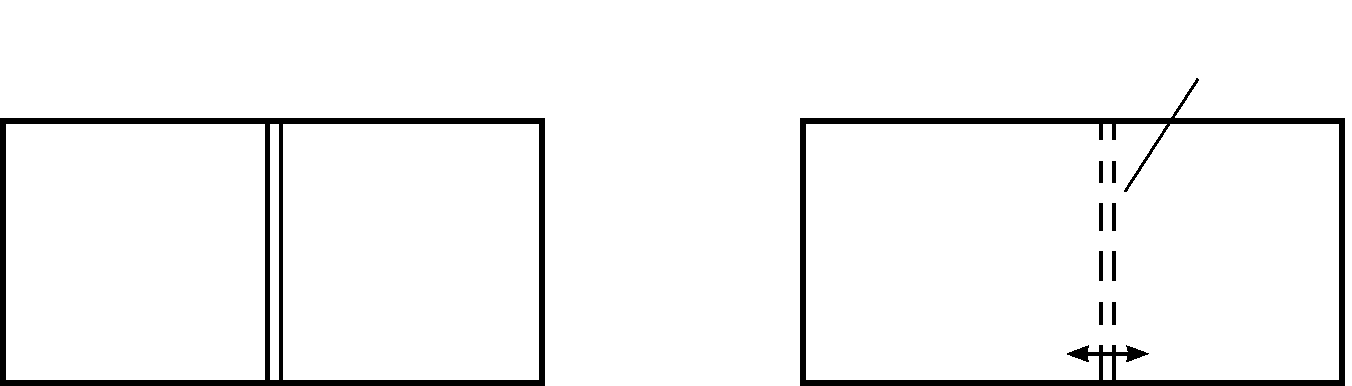
\includegraphics[width=0.3\textwidth]{../img/derivationMu.pdf}
        \caption{caption}  % TODO caption
        \label{img:derivationMu}
    \end{center}
\end{figure}
Energie-, Volumen- und Teilchenaustausch.
\begin{equation}
    \begin{split}
        \difd S_1 &= \pdi{S_1}{E_1}{V_1, N_1} \difd E_1 + \pdi{S_1}{V_1}{E_1, N_1} \difd V_1 + \pdi{S_1}{N_1}{E_1, V_1} \difd N_1 \\
        & \Rightarrow \difd E_1 = \underbrace{T_1 \difd S_1}_{\delta Q} - \underbrace{p_1 \difd V_1}{\text{mech. Arbeit}}
        \underbrace{- T_1 \pdi{S_1}{N_1}{E_1, V_1}}_{\mu_1} \difd N1
    \end{split}
\end{equation}
$\mu$: Chemisches Potential
\begin{equation}
    \Rightarrow E_1 = \delta Q_1 - p_1 \difd V_1 + \mu_1 \difd N_1
\end{equation}
\begin{equation}
    \mu = - T_1 \pdi{S_1}{N_1}{E_1, V_1}
\end{equation}
Im Gleichgewicht, wie oben, folgt $\mu_1 = \mu_2$.

\subsubsection{Fundamentale Gleichung}
\begin{equation}
    \label{eq:fundamentalEQ}
    \difd E = T \difd S - p \difd V + \mu \difd N
\end{equation}
$E(S, V, N)$ ist eine Funktion von \emph{extensiven} Variablen.

\subsubsection{Anwendungsbeispiele}
\begin{enumerate}
    \item Entropie des idealen Gases (einatomig) \\
    Konstante Teilchenzahl $N$
    \begin{equation}
        \begin{split}
            & T \difd S = \difd E + p \difd V, \qquad p V = N k T, \qquad E = \frac{3}{2} N k T \\
            & \Rightarrow \difd S = \frac{\difd E}{T} + \frac{p}{T} \difd V = \frac{3}{2} N k \frac{\difd E}{E} + N k \frac{\difd V}{V}
        \end{split}
    \end{equation}
    $\difd S$ totales Differential:
    \begin{equation}
        \Rightarrow S - S_0 = \frac{3}{2} N k \ln (\frac{E}{E_0}) + N k \ln (\frac{V}{V_0})
    \end{equation}
    Bemerkung: $S$ extensiv (korrekt!), da Ausdruck proportional zu $N$.
    \paragraph{Adiabate} Linien konstanter Entropie \\
    Hier: $\ln(E^{3/2} V) = \const \Leftrightarrow E^{3/2} V = \const$ \\
    Äquivalente Schreibweise: $T^{3/2} V = \const \Leftrightarrow p^{3/2} V^{3/2} V = \const$ \\
    $\Leftrightarrow p^{3/2} V^{5/2} = \const \Leftrightarrow p V^{5/3} = \const$
    \begin{figure}[H]
        \begin{center}
            \includegraphics[width=\textwidth]{../img/adiabate_pV_ST.pdf}
            \caption{caption}  % TODO caption
            \label{img:adiabate_pV_ST}
        \end{center}
    \end{figure}
    \item Gleichheit der absoluten Temperatur $T$ und der Temperatur des idealen Gases $T_G$
    Denkbar ist $T_G = f(T)$
    \begin{equation}
        \begin{split}
            & \difd S = \frac{1}{T} \difd E + \frac{p}{T}\difd V \qquad \text{Integrabilitätsbedingung} \\
            & \frac{\partial}{\partial E} \left( \frac{p}{T} \right)_V = \frac{\partial}{\partial V} \left( \frac{1}{T} \right)_E = 0 \quad \text{da } E = \frac{3}{2} N k T_G
        \end{split}
    \end{equation}
    Ideales Gas: $p V = N k T_G$
    \begin{equation}
        \begin{split}
            \Rightarrow & \frac{\partial}{\partial E} \left( \frac{p}{T} \right)_V = \frac{N k }{V} \frac{\partial}{\partial E} \left( \frac{T_G}{T} \right)_V = 0 \\
            \Rightarrow & \frac{\partial}{\partial T_G} \left( \frac{T_G}{T} \right) = 0 \\
            \Rightarrow & T_G = T \cdot \const
        \end{split}
    \end{equation}
    Die Konstante wird durch den Tripelpunkt des Wassers fixiert.
    \item \emph{Wirkungsgrad} einer Wärmekraftmaschine
    \begin{figure}[H]
        \begin{center}
            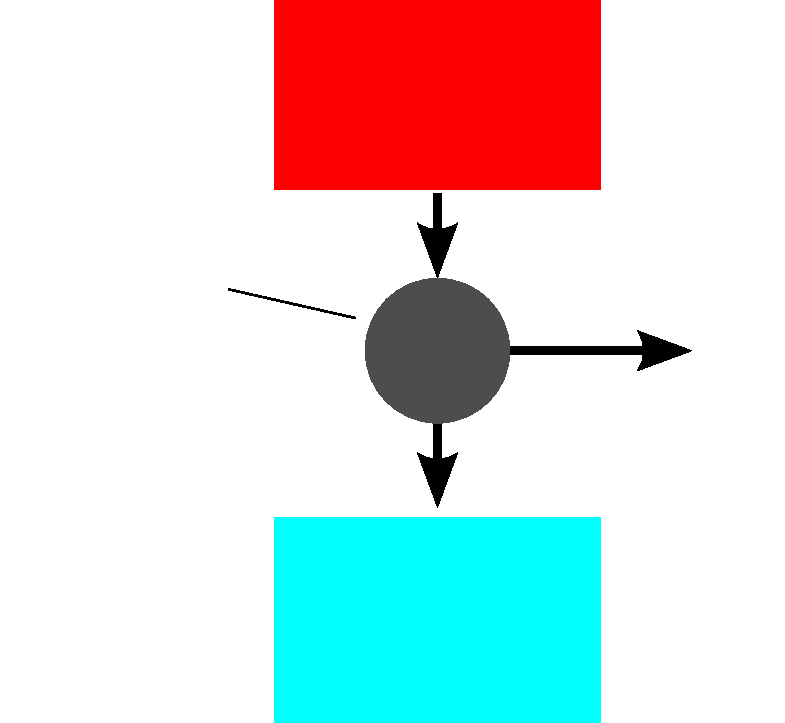
\includegraphics[width=0.3\textwidth]{../img/waermekraftmaschine.pdf}
            \caption{Wärmekraftmaschine.}
            \label{img:waermekraftmaschine}
        \end{center}
    \end{figure}
    
    \begin{figure}[H]
        \begin{center}
            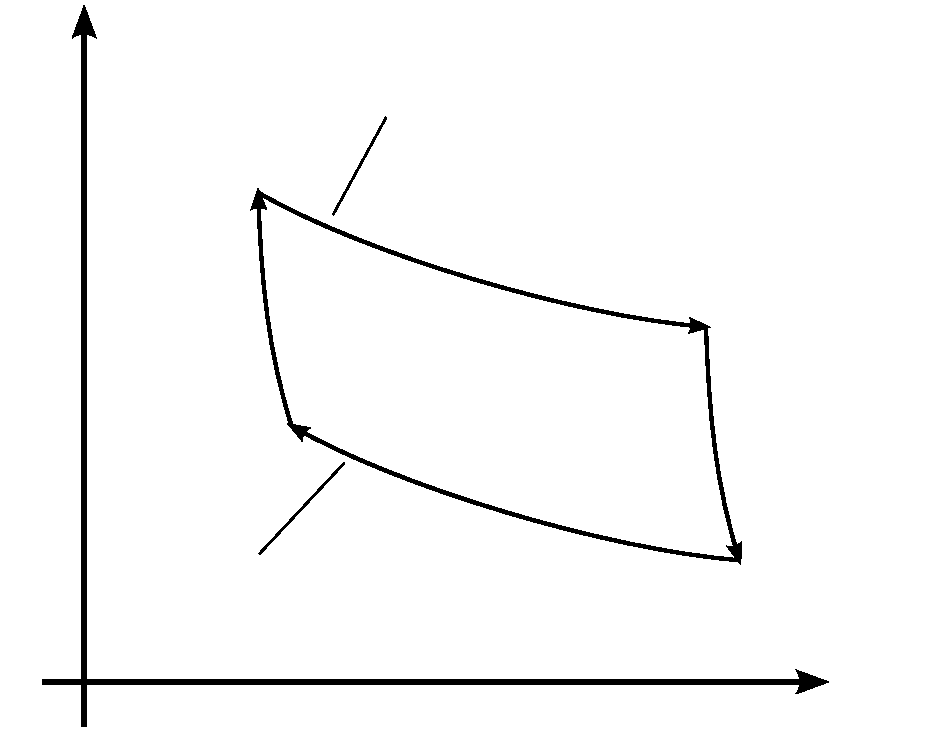
\includegraphics[width=0.3\textwidth]{../img/carnotprocess.pdf}
            \caption{Carnot-Prozess.}
            \label{img:carnot}
        \end{center}
    \end{figure}
    
    Reversibel:
    \begin{equation}
        \begin{split}
            & \Delta S = 0 \Rightarrow - \frac{Q_2}{T_2} + \frac{Q_1}{T_1} = 0  \\
            & \Rightarrow \frac{Q_2}{T_2} = \frac{Q_1}{T_1} = \gamma
        \end{split}
    \end{equation}
    Energieerhaltung (Maschine soll nach \emph{Zyklus} im Ausgangszustan sein $\Rightarrow A = Q_2 - Q_1$) \\
    Wirkungsgrad $\eta$:
    \begin{equation}
        \eta := \frac{A}{Q_2} \Rightarrow \eta_{\text{reversibel}} = \frac{Q_2 - Q_1}{q_2} = \frac{T_2 - T_1}{T_2}
    \end{equation}
    Wärmepumpe:
    \begin{equation}
        \bar{\eta} = \frac{Q_1}{A} (\text{für } T_1 > T_2) \Rightarrow \bar{\eta}_{\text{reversibel}} = \frac{T_1}{T_1 - T_2}
    \end{equation}
    Kühlmaschine:
    \begin{equation}
        \bar{\bar{\eta}} = \frac{Q_2}{-A} (\text{für } T_1 > T_2) \Rightarrow \bar{\bar{\eta}}_{\text{reversibel}} = \frac{T_2}{T_1-T_2}
    \end{equation}
    irreversibel:
    \begin{equation}
        \Delta S > 0 \Rightarrow \frac{Q_1'}{T_1} > \frac{Q_2'}{T_2}
    \end{equation}
    Wirkungsgrad der Wärmekraftmaschine: $\eta_{\text{irrev.}} = \frac{A'}{Q_2'}$ \\
    Sei z.B. $Q_2' = Q_2 \Rightarrow Q_1' > Q_1$
    \begin{equation}
        \begin{split}
            \Rightarrow & A' = Q_2' - Q_1' = Q_2 - Q_1' < A \\
            \Rightarrow & \eta_\text{irrev.} < \eta_\text{reversibel}
        \end{split}
    \end{equation}
    Wirkungsgrad der idealen \emph{Carnot-Maschine} ist maximal.
\end{enumerate}

\subsection{Einige Folgerungen aus den Hauptsätzen}
\subsubsection{Wichtige abgeleitete Größen}
\begin{itemize}
    \item Spezifische Wärme
    \begin{equation}
        \begin{split}
            c_p &= \left( \frac{\Delta Q}{\Delta T} \right)_p = T \left( \frac{\partial S}{\partial T} \right)_p \\
            c_V &= \left( \frac{\Delta Q}{\Delta T} \right)_V = T \left( \frac{\partial S}{\partial T} \right)_V
        \end{split}
    \end{equation}
    Technische Definition bezogen auf 1 Mol, $N=N_A$ (Avogadro) \\
    Korrekterweise: $s = \frac{S N_A}{N}, \quad v = \frac{V N_A}{N}$, siehe Adam + Hittmair \\
    hier sehen wir davon ab
    \item Kompressibilität
    \begin{equation}
        \begin{split}
            \kappa_s &= - \frac{1}{V} \left( \frac{\partial V}{\partial p} \right)_S \text{ (adiabatisch)} \\
            \kappa_T &= - \frac{1}{V} \left( \frac{\partial V}{\partial p} \right)_T \text{ (isotherm)}
        \end{split}
    \end{equation}
    \item Ausdehnungskoeffizient
    \begin{equation}
        \alpha = \frac{1}{V} \left( \frac{\partial V}{\partial T} \right)_p
    \end{equation}
    \item Magnetische Suszeptibilität
    \begin{equation}
        \chi = \left( \frac{\partial M}{\partial H} \right)_T
    \end{equation}
\end{itemize}
Diese Größen sind der Messung direkt zugänglich. Man beachte: die verschiedenen Größen sind nicht unabhängig, z.B. gilt
$c_p - c_v = V T \alpha^2 / \kappa_T$ (Beweis später).
Woher kommen diese Abhängigkeiten? \emph{Integrabilitätsbeziehungen}!
\subsubsection{Maxwell-Beziehungen}
Fundamentale Gleichung \eqref{eq:fundamentalEQ}:
\begin{equation}
    \difd E = T \difd S - p \difd V + \mu \difd N, \quad E=E(S, V, N)
\end{equation}
\paragraph{Freie Energie} $F:=E - TS$ (\textsc{Legendre}-Transformation)
\begin{equation}
    \begin{split}
        \Rightarrow & \difd F = \difd E - T \difd S - S \difd T \\
        \Rightarrow & \difd F = -S\difd T - p \difd V + \mu \difd N \\
        \Rightarrow & F=F(T, V, N)
    \end{split}
\end{equation}
\paragraph{Enthalpie} $H:=E+pV$
\begin{equation}
    \begin{split}
        \Rightarrow & \difd H = \difd E + p \difd V + V \difd p \\
        \Rightarrow & \difd H = T \difd S + V \difd p + \mu \difd N \\
        \Rightarrow & H=H(S, p, N)
    \end{split}
\end{equation}
\paragraph{Freie Enthalpie} $G:=E-T+pV$
\begin{equation}
    \begin{split}
        \Rightarrow & \difd G = - S \difd T + V \difd p + \mu \difd N \\
        \Rightarrow & G=G(T, p, N)
    \end{split}
\end{equation}
$E, F, H, G$ heißen \emph{Thermodynamische Potentiale}.
\paragraph{Integrabilitätsbeziehungen} \mbox{}\\
aus $E$:
\begin{equation}
    \left( \frac{\partial T}{\partial V} \right)_{S, N} = \left( \frac{\partial p}{\partial S} \right)_{V, N}, \quad
    \left( \frac{\partial T}{\partial N} \right)_{S, V} = \left( \frac{\partial \mu}{\partial S} \right)_{V, N}, \quad
    - \left( \frac{\partial p}{\partial N} \right)_{S, V} = \left( \frac{\partial \mu}{\partial V} \right)_{S, N}
\end{equation}
aus $F$:
\begin{equation}
    \left( \frac{\partial S}{\partial V} \right)_{T, N} = \left( \frac{\partial p}{\partial T} \right)_{V, N}, \quad \text{usw.}
\end{equation}
aus $H$:
\begin{equation}
    \left( \frac{\partial T}{\partial p} \right)_{S, N} = \left( \frac{\partial V}{\partial S} \right)_{p, N}, \quad \text{usw.}
\end{equation}
aus $G$:
\begin{equation}
    - \left( \frac{\partial S}{\partial p} \right)_{T, N} = \left( \frac{\partial V}{\partial T} \right)_{p, N}, \quad \text{usw.}
\end{equation}
\textsc{Maxwell}-Beziehungen (insgesamt 12 Beziehungen)
\subsubsection{Exkurs: Variablentransformation}
Erwünscht:
\begin{equation}
    \left( \frac{\partial E}{\partial V} \right)_T \overset{?}{\rightarrow} \left( \frac{\partial E}{\partial V} \right)_p
    \text{ oder }
    \left( \frac{\partial E}{\partial V} \right)_T \overset{?}{\rightarrow} \left( \frac{\partial E}{\partial p} \right)_T
\end{equation}
Wichtig: Jacobi'sche Determinanten $f=f(x, y)$; $g=g(x, y)$ \\
Definition:
\begin{equation}
    \frac{\partial (f, g)}{\partial(x, y)} = \det
    \begin{pmatrix}
\frac{\partial f}{\partial x} & \frac{\partial f}{\partial y} \\
\frac{\partial g}{\partial x} & \frac{\partial g}{\partial y}
\end{pmatrix}
= \left( \frac{\partial f}{\partial x} \right) \left( \frac{\partial g}{\partial
y} \right) - \left( \frac{\partial f}{\partial y} \right) \left( \frac{\partial g}{\partial x} \right)
\end{equation}
Rechenregeln
\begin{equation}
    \frac{\partial(f, g)}{\partial(x, y)} = -\frac{\partial(f, g)}{\partial(y, x)}; \qquad
    \frac{\partial(f, y)}{\partial(x, y)} = \frac{\partial f}{\partial x}
\end{equation}
und für $x=(u, v), y=(u, v)$
\begin{equation}
    \Rightarrow \frac{\partial(f, g)}{\partial(u, v)} = \frac{\partial(f, g)}{\partial(x, y)} \cdot \frac{\partial(x, y)}{\partial(u, v)}
\end{equation}
Beweis:
\begin{equation}
    \begin{split}
        \det
        \begin{pmatrix}
\frac{\partial f}{\partial u} & \frac{\partial f}{\partial v} \\
\frac{\partial g}{\partial u} & \frac{\partial g}{\partial v}
\end{pmatrix}
&= \det \left[
\begin{pmatrix}
\frac{\partial f}{\partial x} & \frac{\partial f}{\partial y} \\
\frac{\partial g}{\partial x} & \frac{\partial g}{\partial y}
\end{pmatrix}
\cdot
\begin{pmatrix}
\frac{\partial x}{\partial u} & \frac{\partial x}{\partial v} \\
\frac{\partial y}{\partial u} & \frac{\partial y}{\partial v}
\end{pmatrix}
\right] \\
&= \det
\begin{pmatrix}
\frac{\partial f}{\partial x} & \frac{\partial f}{\partial y} \\
\frac{\partial g}{\partial x} & \frac{\partial g}{\partial y}
\end{pmatrix}
\cdot \det
\begin{pmatrix}
\frac{\partial x}{\partial u} & \frac{\partial x}{\partial v} \\
\frac{\partial y}{\partial u} & \frac{\partial y}{\partial v}
\end{pmatrix} \qquad \square
    \end{split}
\end{equation}
Spezialfall der Kettenregel:
\begin{equation}
    \frac{\partial(f, g)}{\partial(x, y)} \cdot \frac{\partial(x, y)}{\partial(f, g)} = 1
\end{equation}
\subsubsection{Anwendungsbeispiele} $N$ = konstant
\begin{enumerate}  % a), b)
    \item
    \begin{equation}
        \begin{split}
            c_p &=  T \left( \frac{\partial S}{\partial T} \right)_p = T \frac{\partial(S, p)}{\partial(T, p)} \overset{\text{$V$ abh.}}{=}
            T \frac{\partial(S, p)}{\partial(T, V)} / \underbrace{\frac{\partial(T, p)}{\partial(T, V)}}_{ \left( \frac{\partial p}{\partial V} \right)_T} \\
            &= \frac{T}{ \left( \frac{\partial p}{\partial V} \right)_T} \left[ \left( \frac{\partial S}{\partial T} \right)_V
            \left( \frac{\partial p}{\partial V} \right) - \left( \frac{\partial S}{\partial V} \right)_T \left( \frac{\partial p}{\partial T} \right)_V \right] \\
            &= c_V - T \left( \frac{\partial S}{\partial V} \right)_T \left( \frac{\partial p}{\partial T} \right)_V / \left( \frac{\partial p}{\partial V} \right)_T \\
            &\overset{\text{Maxwell-Bez.}}{=} c_V - T \left( \frac{\partial p}{\partial T} \right)_V^2 / \left( \frac{\partial p}{\partial V} \right)_T
        \end{split}
    \end{equation}
    Nun ist
    \begin{equation}
        \begin{split}
            \left( \frac{\partial p}{\partial T} \right)_V &= \frac{\partial(p, V)}{\partial (T, V)} \\
            &= \frac{\partial (p, V)}{\partial (p, T)} \cdot \frac{\partial(p, T)}{\partial(T, V)} \\
            &= \left( \frac{\partial V}{\partial T} \right)_p \cdot \left[ - \left( \frac{\partial p}{\partial V} \right)_T \right]
        \end{split}
    \end{equation}
    \begin{equation}
        \Rightarrow c_p = c_V - T \left( \frac{\partial V}{\partial T} \right)_p^2 \left( \frac{\partial p}{\partial V} \right)_T = c_V + T V \alpha^2 / \kappa_T^2
    \end{equation}
    \item
    \begin{equation}
        \frac{c_p}{c_v} = \frac{\kappa_T}{\kappa_S} \quad \text{(Übungsaufgabe)}
    \end{equation}
\end{enumerate}
\subsubsection{Die Gibbs-Duhem-Beziehung}
Fundamentalgleichung (\autoref{eq:fundamentalEQ}), $E, S, V, N$ sind extensive Variablen
\begin{equation}
    \difd E = T \difd S - p \difd V + \mu \difd N
\end{equation}
Somit gilt für $E=E(S, V, N)$ dass $E(\alpha S, \alpha V, \alpha N) = \alpha E(S, V, N)$ (homogene Funktion nach \textsc{Euler})
\paragraph{Eulerscher Satz über homogene Funktion} $f(x_1, \ldots, x_n)$: \\
Falls $f(\alpha x_1, \ldots, \alpha x_n) = \alpha^r f(x_1, \ldots, x_n)$ so ist
\begin{equation}
    \sum_{i=1}^{n} x_i \frac{\partial f}{\partial x_i} = r f
\end{equation}
Beweis: Differentiation nach $\alpha$ und dann $\alpha = 1$ setzten.
\paragraph{Fundamentalrelation}\mbox{}\\
Damit folgt
\begin{equation}
    \begin{split}
        E &= \left( \frac{\partial E}{\partial S} \right)_{V, N} S + \left( \frac{\partial E}{\partial V} \right)_{S, N} V + \left( \frac{\partial E}{\partial N} \right)_{V, S} N \\
        &= T S - p V + \mu N
    \end{split}
\end{equation}
Damit, im Gleichgewicht
\begin{equation}
    E = T S - p V + \mu N \qquad \text{Fundamentalrelation}
\end{equation}
Differentiation ergibt:
\begin{equation}
    \difd E = T \difd S + S \difd T - p \difd V - V \difd P + \mu \difd N + N \difd \mu
\end{equation}
\begin{equation}
    \Rightarrow S \difd T - V \difd p + N \difd \mu = 0 \qquad \text{\textsc{Gibbs-Duhem} Beziehung}
\end{equation}
D.h. $T$, $p$ und $\mu$ nicht unabhängig voneinander. \\
Folgerung: Die Zustandsgleichung muss zur eindeutigen Charakterisierung des Systems zumindest \emph{eine} extensive Größe enthalten. \\
Folgerungen für die thermodynamischen Potentiale:
\begin{equation}
    \begin{split}
        & E(S, V, N) = T S - p V + \mu N \\
        & F(T, V, N) = E - TS = - pV + \mu N \\
        & H(S, p, N) = E + p V = T S + \mu N \\
        & G(T, p, N) = E + p V - T S = \mu N
    \end{split}
\end{equation}
Man beachte: obwohl $G=\mu N$ recht einfach erscheint, ist zur Kennzeichnung des Systems die Kenntnis von $\mu$ als Funktion der \emph{natürlichen}
Variablen $T, p, N$, d.h. die Funktionalität $\mu(T, p, N)$ notwendig.

\subsubsection{Der Joule-Thomson-Prozess (gedrosselte Entspannung)}
\begin{figure}[H]
    \begin{center}
        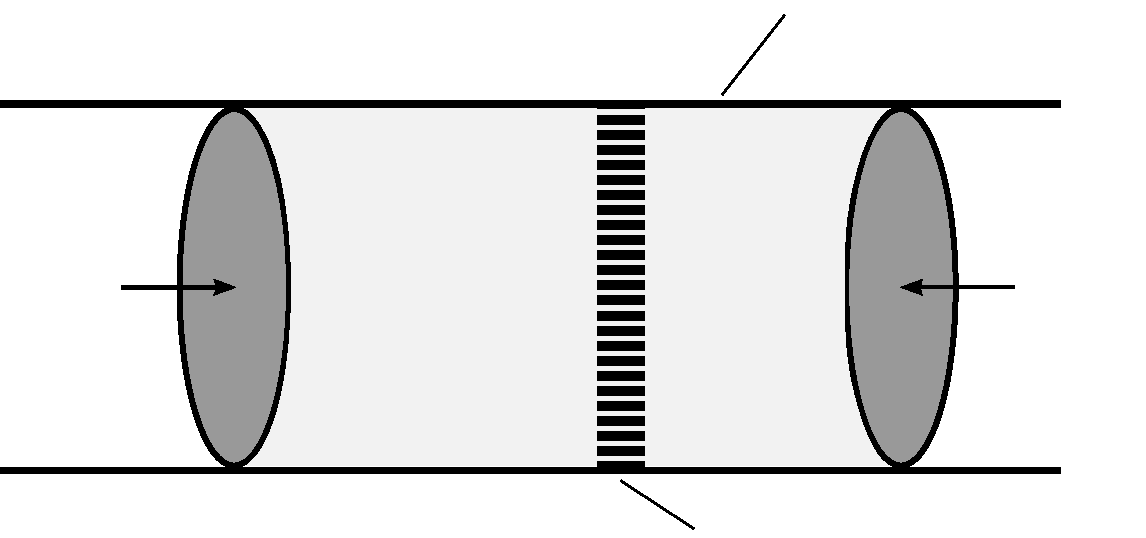
\includegraphics[width=0.3\textwidth]{../img/joule-thomson-process.pdf}
        \caption{Joule-Thomson-Prozess.}
        \label{img:joule-thomson-process}
    \end{center}
\end{figure}
Gasströmung bei konstant gehaltenen Druckwerten $p_1, p_2$. Irreversibler Prozess, keine Strömungsenergie wegen Drossel.
\begin{equation}
    \begin{split}
        \difd E &= \difd E_1 + \difd E_2 = - p_1 \difd V_1 - p \difd V_2 \\
        & \overset{p_1, p_2 = \const}{=} - \difd (p_1 V_1) - \difd (p_2, V_2) \\
        & \Rightarrow \difd (E_1 + p_1 V_1) + \difd (E_2 p_2 V_2) = 0
    \end{split}
\end{equation}
$\Rightarrow$ Die Gesamtenthalpie $H = E + p V$ bleibt erhalten.\\
Von Interesse: Temperaturänderung bei Druckänderung. Infinitesimal verrücken.
\begin{equation}
    \frac{\Delta T}{\Delta p} \to \pdi{T}{p}{N, H} \equiv \kappa_\text{JT}
\end{equation}
Berechnung ($N$ konstant)
\begin{equation}
    \begin{split}
        \pdi{T}{p}{H} &= \pd{(T, H)}{(p, H)} = \pd{(T, H)}{(T, p)} \cdot \pd{(T, p)}{(p, H)} \\
        &= - \pdi{H}{p}{T} / \pdi{H}{T}{p} \\
        \difd H &= T \difd S + V \difd p = T \pdi{S}{T}{p} \difd T + \left[ T \pdi{S}{p}{T} + V \right] \difd p \\
        & \Rightarrow \pdi{H}{T}{p} = T \pdi{S}{T}{p} = c_p \\
        \pdi{H}{p}{T} &= V + T \pdi{S}{p}{T} = V - T \pdi{V}{T}{p} \text{ (mit Maxwellbeziehung zu $G$)} \\
        &= V \left[ 1 - T \alpha \right]
    \end{split}
\end{equation}
Damit
\begin{equation}
    \kappa_\text{JT} = \frac{V \left( T \alpha - 1 \right) }{c_p}
\end{equation}
Im Versuch ist $\delta p$ negativ (Druckverminderung)
\begin{equation}
    \Rightarrow
    \begin{cases}
        \kappa_\text{JT} > 0 & \text{Temperaturabnahme} \\
        \kappa_\text{JT} < 0 & \text{Temperaturzunahme} \\
    \end{cases}
\end{equation}
\begin{enumerate}[a)]  % TODO alpha
    \item Ideales Gas
    \begin{equation}
        \begin{split}
            \alpha &= \frac{1}{V} \pdi{V}{T}{p} = \frac{1}{V} \frac{N k}{p} = \frac{N k}{N k T} = \frac{1}{T} \\
            & \Rightarrow T \alpha - 1 = 0 \Rightarrow \kappa_\text{JT} = 0
        \end{split}
    \end{equation}
    \item van-der Waals Gas: Hier, i.A. ist $\kappa_\text{JT} \neq 0$ (hängt von $p, T$ ab) \\
    Die Kurve, für die $\kappa_\text{JT} = 0 $ gilt, heißt \emph{Inversionskurve}. Kühleffekte nur innerhalb
    $\kappa_\text{JT} > 0$
\end{enumerate}

\subsection{Thermodynamische Potentiale}
Bereits kennengelernt $E(S, V, n), F(T, V, N), H(S, p, N), G(T, p, N)$ und Varianten, z.B. $S(E, V, N)$. Die obigen Potentiale
sind durch sogenannte \emph{Legendre-Transformationen} miteinander verknüpft. \\
Allgemeines Schema: Sei $P(x_1, \ldots, x_n)$ ein thermodynamisches Potential mit
\begin{equation}
    \difd P = K_1 \difd x_1 + K_2 \difd x_2 + \ldots + K_n \difd x_n
\end{equation}
Dann ist $Q_i := P - K_i x_i$ neues thermodynamisches Potential mit
\begin{equation}
    \begin{split}
        \difd Q_i &= K_1 \difd x_1 + \ldots + K_i \difd x_i + \ldots + K_n \difd x_n - K_i \difd x_i - x_i \difd K_i \\
        & = K_1 \difd x_1 + \ldots - x_i \difd K_i + \ldots + K_n \difd x_n
    \end{split}
\end{equation}
d.h. $Q_i = Q(x_1, \ldots, x_{i-1}, K_i, x_{i+1}, \ldots, x_n)$ und
\begin{equation}
    \pdi{Q_1}{x_1}{x_2, \ldots, K_i, \ldots, x_n} = K_1, \ldots, \pdi{Q}{K_i}{x_1, \ldots, x_i, \ldots x_n} % TODO letztes x_i durchgestrichen
\end{equation}
Die beiden Potentiale $P$ und $Q$ enthalten die gleichen Information. Es ist eine Frage der Zweckmäßigkeit, welches thermodynamisches Potential
im Spezialfall benutzt wird. \\
$x_1, \ldots, x_i, \ldots, x_n \to $ natürliche Variable von $P$; \\
$x_1, \ldots, k_i, \ldots, x_n \to$ natürliche Variable von $Q_i$ \\
Zum Informationsverlust bei beliebigen Transformationen und zur heuristischen Begründung der Legendre-Transformation siehe z.B. A. u. H. §3.23. \\[\baselineskip]
Damit enthalten $E, F, G$ und $H$ als Funktion ihrer natürlichen Variablen die gleiche INformation
\begin{equation}
    \begin{split}
        & F(T, V, N) = E - ST \\
        & G(T, p, N) = F + p V = E - ST + pV \\
        & H(S, p, N) = E + pV
    \end{split}
\end{equation}
Bedeutung:
\begin{description}
    \item[$F$] \emph{isotherme Prozesse}: Freie Energie; Anteil der Gesamtenergie, der zur Arbeitsleistung verwendet werden kann
    \item[$G$] \emph{isotherm-isobare Prozesse}: Freie Enthalpie (Gibbssches Potential); Wichtig für chemische Prozesse.
    \item[$H$] \emph{adiabatisch-isobare Prozesse}
\end{description}
Es gibt weitere thermodynamische Potentiale, z.B. das \emph{großkanonische} Potential $\Omega = \Omega(T, V, \mu)$.
\begin{equation}
    \begin{split}
        \Omega(T, V, \mu) &= F - \mu N \\
        \Rightarrow \difd \Omega &= - S \difd T - p \difd V - N \difd \mu
    \end{split}
\end{equation}
Fundamentalbeziehung $F=-pV + \mu N$
\begin{equation}
    \Rightarrow \Omega = - p V
\end{equation}
Vorsicht: $p$ ist \emph{keine} natürliche Variable von $\Omega$; für die Kenntnis des Systems brauchen wir $p(T, V, \mu)$.\\[\baselineskip]
Ein Beispiel zum Zurückrechnen: $\Omega$ ist bekannt; wie sieht $E$ aus? \\
$\Omega(T, V, \mu)$ bekannt:
\begin{equation}
    \begin{split}
        S &= \pdi{\Omega}{T}{V, \mu} \\
        N &= \pdi{\Omega}{\mu}{T, V} \\
        \Rightarrow &
        \begin{cases}
            S(T, V, \mu) \\
            N(T, V, \mu)
        \end{cases} \\
        \Rightarrow &
        \begin{cases}
            T = T(S, V, N) \\
            \mu = \mu(S, V, N)
        \end{cases} \\
        \Rightarrow & E(S, V, N) = \Omega + TS + \mu N \\
        &= \Omega(T(S, V, N), V, \mu(S, V, N)) + T(S, V, N) S + \mu (S, V, N) N
    \end{split}
\end{equation}
\begin{equation}
    \begin{array}{lll}
E & \difd E = T \difd S - p \difd V + \mu \difd N & E(S, V, N) \\
F = E - TS & \difd F = - S \difd T - p \difd V + \mu \difd N & F(T, V, N) \\
H = E + pV & \difd H = T \difd S + V \difd p + \mu \difd N & H(S, p, N) \\
G = E - TS + pV & \difd G = - S \difd T + V \difd p + \mu \difd N & G(T, p, N) \\
\Omega = E - TS - \mu N & \difd \Omega = - S \difd T - p \difd V - N \difd \mu & \Omega(T, V, \mu)
\end{array}
\end{equation}
Es gibt noch weitere zwei thermodynamische Potentiale, welche allerdings ungebräuchlich sind.

\subsection{3. Hauptsatz der Thermodynamik}
Auch bekannt als \textsc{Nerst}'sches Theorem (1906) \\
Die Entropie eines homogenen, realen Stoffes ist bei $T=0$ Null. \\
Mathematisch formuliert:
\begin{equation}
    \lim_{T \to 0} S(T, V) = 0, \qquad \lim_{T \to 0} S(T, P) = 0
\end{equation}
Erfahrungssatz der Thermodynamik. Beweis: Quantenstatistik. \\[\baselineskip]
Bemerkung: Der 3. Hauptsatz gilt nicht für das ideale Gas.
\subsubsection{Folgerungen aus dem 3. Hauptsatz}
\begin{enumerate}[i)]
    \item Der Satz gilt für alle $V$ und $p$, somit
    \begin{equation}
        \lim_{T \to 0} \pdi{S}{V}{T} = 0, \qquad \lim_{T \to 0} \pdi{S}{p}{T} = 0
    \end{equation}
    \item Sei $C_\xi$ die spezifische Wärme ($\xi = p$ oder $V$), $c_\xi = T \pdi{S}{T}{\xi}$. Entlang eines reversiblen Weges ist
    \begin{equation}
        S(T, \xi) = \int_{0}^{T} c_\xi(T') \frac{\difd T'}{T'} + \underbrace{S(T=0, \xi)}_{=0, \text{ mit 3. HS}}
    \end{equation}
    Damit $\lim_{T \to 0} S(T, \xi) = 0$ ist, muss gelten:
    \begin{equation}
        \begin{split}
            & \lim_{T \to 0} c_\xi(T) = 0 \\
            \Rightarrow & c_V (T=0) = 0 = c_p(T=0)
        \end{split}
    \end{equation}
    \item Ausdehnungskoeffizient $\alpha$
    \begin{equation}
        \lim_{T \to 0} \alpha = \lim_{T \to 0} \frac{1}{V} \pdi{V}{T}{p} = - \lim_{T \to 0} \frac{1}{V} \pdi{S}{p}{T} = 0
    \end{equation}
    Weiterhin ist mit $\pdi{p}{V}{T} \pdi{T}{p}{V} \pdi{V}{T}{p} = -1 \, (*)$:
    \begin{equation}
        \begin{split}
            & \lim_{T \to 0} \frac{c_p - c_V}{T} = \lim_{T \to 0} \left[ \pdi{S}{V}{T} \pdi{p}{T}{V} \pdi{p}{V}{T} \right] \\
            &\overset{(*)}{=} \lim_{T \to 0} \left\{ \pdi{S}{V}{T} \left[- \pdi{V}{T}{p} \right] \right\} \\
            &= \lim_{T \to 0} \left\{ \pdi{S}{V}{T} \pdi{S}{p}{T} \right\} = 0
        \end{split}
    \end{equation}
    \item Der absolute Nullpunkt ist unerreichbar, nur \emph{asymptotische} Annäherungen möglich. In Frage kommen nur adiabatische Prozesse,
    z.B. adiabatische Expansion
    \begin{equation}
        \begin{split}
            0 &= T \difd S = T \pdi{S}{T}{p} \difd T + T \pdi{S}{p}{T} \difd p \\
            &= c_p \difd T - T \pdi{V}{T}{p} \difd p \\
            &= c_p \difd T - \alpha V T \difd p \\
            \Rightarrow & \Delta T = \frac{\alpha V T}{c_p} \Delta p
        \end{split}
    \end{equation}
    Führt eine Druckänderung $\Delta p$ zu einer Temperaturänderung $\Delta T$ in der Nähe von $T=0$ ?
    Gesucht: Wert von $\lim_{T \to 0} \frac{\alpha V T}{c_p}$.\\
    Nun ist $c_p \propto T^x \ (x > 0)$ für kleine $T$, dann auch $S \propto T^x$ (da $c_p = T \pdi{S}{T}{p}$) und
    $V \alpha \propto T^x$ (siehe iii)). Somit:
    \begin{equation}
        \lim_{T \to 0} \frac{\alpha V}{c_p} = \const \Rightarrow \lim_{T \to 0}  \frac{\alpha V T}{c_p} = 0
    \end{equation}
    Hinweis: Experimentell verwendet man die adiabatische Entmagnetisierung einer paramagnetischen Substanz
    \begin{figure}[H]
        \begin{center}
            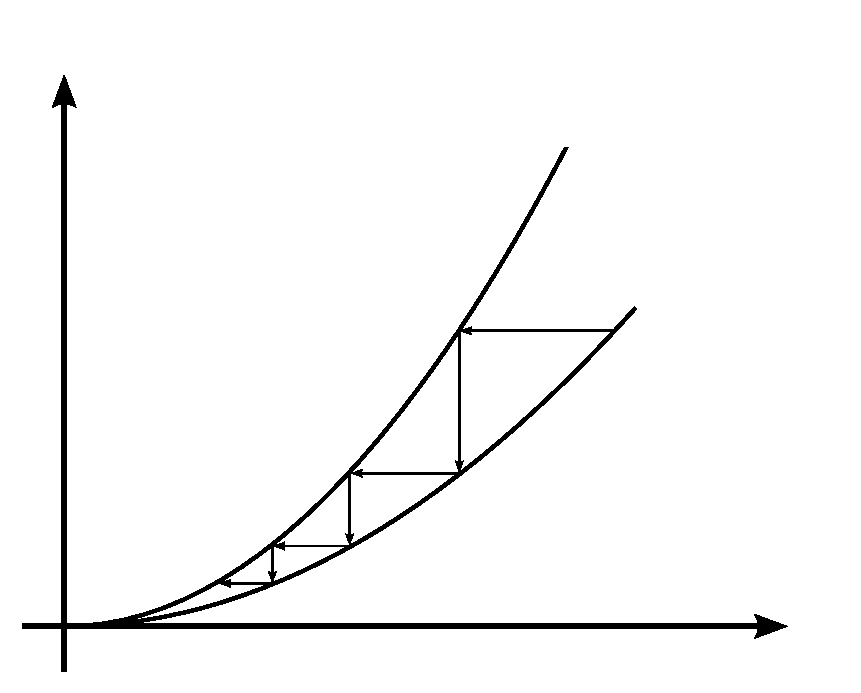
\includegraphics[width=0.3\textwidth]{../img/paramag_Tto0.pdf}
            \caption{caption}  % TODO caption
            \label{img:paramag_Tto0}
        \end{center}
    \end{figure}
    \item Weitere Folgerungen
    \begin{itemize}
        \item Da $F = E - TS$, hat man $F = E$ im Grenzfall $T \to 0$
        \begin{equation}
            \begin{split}
                \difd F &= - S \difd T - p \difd V \Rightarrow \lim_{T \to 0} \pdi{F}{T}{V} = \lim_{T \to 0} (-S) = 0 \\
                \difd E &= \difd F + T \difd S + S \difd T \\
                \Rightarrow & \lim_{T \to 0} \pdi{E}{T}{V} = \lim_{T \to 0} \pdi{E}{T}{V}
                + \lim_{T \to 0} \underbrace{\left[ T \pdi{S}{T}{V} \right]}_{c_V} + \lim_{T \to 0} S = 0
            \end{split}
        \end{equation}
        \begin{equation}
            \begin{split}
                & E(T, V) = \int_{0}^{T} c_V \difd T' + E(0, V) \text{ mit } c_V > 0 \\
                &\Rightarrow E(T, V) > E(0, V) \text{ für } T > 0, T \text{ klein} \\
                & F(T, V) = E(T, V) - T \int_{0}^{T} \frac{c_V}{T'} \difd T' \\
                & = \underbrace{E(0, V)}_{=F(0, V)} - T \int_{0}^{T} \underbrace{\left( \frac{c_V}{T'} - \frac{c_V}{T} \right)}_{>0} \difd T'
            \end{split}
        \end{equation}
        \begin{figure}[H]
            \begin{center}
                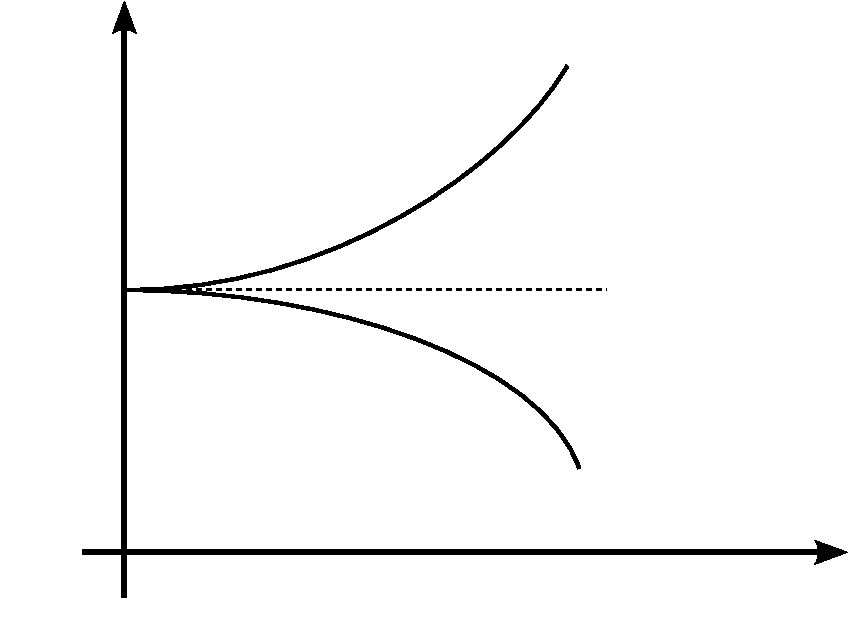
\includegraphics[width=0.3\textwidth]{../img/FandEoverT.pdf}
                \caption{caption}  % TODO caption
                \label{img:FandEoverT}
            \end{center}
        \end{figure}
    \end{itemize}
\end{enumerate}

\subsection{Stabilität des Gleichgewichtzustandes}
Im Gleichgewicht ist die Entropie maximal. Von Interesse: Rolle der Fluktuation.
\begin{figure}[H]
    \begin{center}
        \includegraphics[width=0.3\textwidth]{../img/asdf.pdf}
        \caption{caption}
        \label{img:label}
    \end{center}
\end{figure}
\begin{equation}
    \begin{split}
        & \Delta S \simeq \sum_{\alpha = 1, 2} \left[ \pdi{S_\alpha}{E_\alpha}{V_\alpha, N_\alpha} \Delta E_\alpha
        + \pdi{S_\alpha}{V_\alpha}{E_\alpha, V_\alpha} \Delta V_\alpha + \pdi{S_\alpha}{N_\alpha}{E_\alpha, V_\alpha} \Delta N_\alpha \right] \\
        & \Delta E_1 = - \Delta E_2, \quad \Delta V_1 = - \Delta V_2, \quad \Delta N_1 = - \Delta N_2 \\
        & \Delta S \simeq = \left( \frac{1}{T_1} - \frac{1}{T_2} \right) \Delta E_1 + \left( \frac{p_1}{T_1}
        - \frac{p_2}{T_2} \right) \Delta V_1 + \left( \frac{\mu_1}{T_1} - \frac{\mu_2}{T_2} \right) \Delta N_1
    \end{split}
\end{equation}
Gleichgewicht: $S$ maximal $\Rightarrow \Delta S = 0; \Delta E_1, \Delta V_1, \Delta N_1$ sind beliebig
$\Rightarrow T_1 = T_2 \Rightarrow p_1 = p_2$ und $\mu_1 = \mu_2$. \\
Das gleiche Ergebnis folgt, wenn man Änderungen der Energie betrachtet:
\begin{equation}
    \Delta E \simeq \underbrace{\left( T_1 - T_2 \right)  \Delta S_1 - \left( p_1 - p_2 \right) \Delta V_1 + \left( \mu_1 - \mu_2 \right) \Delta N_1}_{\Delta E^{(1)}; \text{linearisierter Ausdruck}} \quad \text{($E$ minimal)}
\end{equation}
Betrachten wir Fluktuationen aus dem Gleichgewicht. Im Gleichgewicht $\Delta E^{(1)} = 0$. \\
Fundamental ist die Rolle der höheren Ableitungen: $\Delta E = \Delta E^{(1)} + \Delta E^{(2)} + \ldots$
\begin{equation}
    \text{so ergibt} \quad
    \begin{cases}
        \Delta E^{(2)} > 0 & \text{stabiler Zustand} \\
        \Delta E^{(2)} < 0 & \text{instabiler Zustand} \\
        \Delta E^{(2)} = 0 & \text{Zustand ist indeterminiert,} \\
        & \text{hängt von den weiteren Ableitungen ab.}
    \end{cases}
\end{equation}
Folgerungen: \\
TODO: Graphik Fluktuation von Wärmeenergie.\\  % TODO Bild
\begin{equation}
    \begin{split}
        & \Delta S_1 = - \Delta S_2 \qquad \text{Fluktuation} \\
        & \Delta V_1 = \Delta V_2 = \Delta N_1 = \Delta N_2 = 0 \\
        & \Rightarrow \Delta E^{(2)} \simeq = \frac{1}{2} \left( \frac{\partial^2 E_1}{\partial S_1^2} \right)_{V_1, N_1} (\Delta S_1)^2 +  
        \left( \frac{\partial^2 E_2}{\partial S_2^2} \right)_{V_2, N_2} (\Delta S_2)^2 
    \end{split}
\end{equation}
Nun ist
\begin{equation}
    \left( \frac{\partial^2 E}{\partial S^2} \right)_{V, N} = \pdi{T}{S}{V, N} = \frac{T}{c_V}  \quad \text{und} \quad
    (\Delta S_1)^2 = (\Delta S_2)^2
\end{equation}
\begin{equation}
    \begin{split}
        \Delta E^{(2)} = \frac{1}{2} (\Delta S_1)^2 \left( \frac{T_1}{C_{V1}} + \frac{T_2}{C_{V2}} \right) = (\Delta S_1)^2 \frac{T_1}{c_{V1}}
    \end{split}
\end{equation}
Aus $\Delta E^{(2)} > 0$ folgt:
\begin{equation}
    c_V > 0
\end{equation} 
Betrachten wir die Fluktuation um $V$ bei konstant gehaltenen $S$ und $N$. \\
Hier ist
\begin{equation}
    \left( \frac{\partial^2 E}{\partial V^2} \right)_{S, N} = - \pdi{p}{V}{S, N} = - \frac{1}{\pdi{V}{p}{S, N}} = \frac{1}{V \kappa_S}
\end{equation}
Wie oben:
\begin{equation}
    \Rightarrow \kappa_S > 0
\end{equation}
$F = E - TS$. Im thermodynamischen Gleichgewicht. $0 \leq \Delta F = \Delta F^{(2)}$ ($F$ minimal im Gleichgewicht, $\Delta F^{(1)} = 0$). \\
Hier ist
\begin{equation}
    \left( \frac{\partial^2 F}{\partial V^2} \right)_{T, N} = - \pdi{p}{V}{T, N} = \frac{1}{V \kappa_T} \Rightarrow \kappa_T > 0
\end{equation}
$H = E + pV$. Hier:
\begin{equation}
    \left( \frac{\partial^2 H}{\partial S^2} \right)_{p, N} = \pdi{T}{S}{p, N} = \frac{T}{c_p} \Rightarrow c_p > 0
\end{equation}
Diese Beispiele sind \emph{Spezialfälle} eines allgemeinen Satzes: \\[\baselineskip]
Sei $\Phi$ entweder die Energie des Systems oder eine Legendre-Transformierte davon. $\Phi$ sei eine Funktion der natürlichen Variablen 
$X_1, \ldots, X_r$ und $I_{r+1}, \ldots, I_n$ ($X_i$ extensiv, $I_j$ intensiv). Damit ist
\begin{equation}
    \difd \Phi = \sum_{i=1}^{r}  I_i \difd X_i - \sum_{j=r+1}^{n} X_j \difd I_j
\end{equation}
und es gelten die \emph{Stabilitätsbedingungen}
\begin{equation}
    0 \leq \pdi{Itext_k}{X_k}{X_i (i \neq k), I_j} \qquad \forall k \qquad \text{(\textsc{Chandler}, Kap. 2)}
\end{equation}\\
Physikalische Deutung: Prinzip von \textsc{Le Chatelier}: Jede spontane Änderung des Systems aus dem Gleichgewicht führt zu Prozessen, die zur 
Wiederherstellung des Gleichgewichts streben. Z.B. Zufuhr von Wärme bei $c_V > 0 \Rightarrow$ lokale Erhöhung von $T \Rightarrow $ 
Ausgleich der Temperatur (Wärmeabfuhr). \\[\baselineskip]
Es gilt:
\begin{equation}
    c_p > c_V > 0
\end{equation}
und
\begin{equation}
    \kappa_T > \kappa_S > 0
\end{equation}

\newpage
\section{Anwendungen der Thermodynamik}
\subsection{Die Misch(ungs)entropie}
Beispiel: Mischung zweier idealer Gase \\
TODO: Bild: 2 Kasten mit Loch \\ %TODO Bild
\begin{equation}
    p = \frac{N_1 k T}{V_1} = \frac{N_2 k T}{V_2} \Rightarrow \frac{N_1}{V_1} = \frac{N_2}{V_2}
\end{equation}
Partialdrucke
\begin{equation}
    p_1 = \frac{N_1 k T}{V}; \quad p_2 = \frac{N_2 k T}{V}
\end{equation}
\textsc{Dalton}sches Gesetz: Der Gesamtdruck $p_G$ it die Summe der Partialdrücke, $p_G = p_1 + p_2$ \\
Hier:
\begin{equation}
    p_G = \frac{N_1 k T}{V} + \frac{N_2 k T}{V} = \frac{p V_1 + p V_2}{V} = p
\end{equation}
Außerdem ändert sich $E_1$ und $E_2$ nicht. \\
Was passiert mit der Entropie? Anfangswerte:
\begin{equation}
    \begin{split}
        & S_1 = S_{10} + \frac{3}{2} N_1 k \ln(E_1) + N_1 k \ln(V_1) \\
        & S_2 = S_{20} + \frac{3}{2} N_2 k \ln(E_2) + N_2 k \ln(V_2) \\
        & S_A = S_1 + S_2 \quad \text{A=Anfang}
    \end{split}
\end{equation}
Was ändert sich nach der Öffnung? $V_1 \to V, V_2 \to V$. Damit ist für $S_E$ ($E=$ Ende):
\begin{equation}
    \begin{split}
        S_E - S_A &= N_1 k \left[ \ln(V) - \ln(V_1) \right] + N_2 k \left[ \ln(V) - \ln(V_2) \right] \\
        &= k N_1 \ln \left( \frac{V}{V_1} \right)  + k N_2 \ln \left( \frac{V}{V_2} \right) \\
        &= k \left[ N_1 \ln \left( \frac{N_G}{N_1} \right) + N_2 \ln \left( \frac{N_G}{N_2} \right)  \right] \quad \text{mit } N_G = N_1 + N_2
    \end{split}
\end{equation}
$\Rightarrow$ Zunahme der Entropie. \\[\baselineskip]
Allgemein: für $m$ ideale Gase
\begin{equation}
    S_E - S_A = k \sum_{i=1}^{m} N_i \ln \left( \frac{N_G}{N_i} \right) \quad \text{mit } N_G = N_1 + \ldots + N_m
\end{equation}
oder mit $n_i$ Molzahl, $N_i = N_A n_i$, $R = k N_A$ (Gaskonstante)
\begin{equation}
    S_E - S_A = R \sum_{i=1}^{m} n_i \ln \left( \frac{n_G}{n_i} \right) \quad n_G = n_1 + \ldots + n_m
\end{equation}
Man beachte: $S_E - S_A > 0$ für $i > 0$; der Prozess ist irreversibel. \\
Was passiert, wenn die zwei Gase identisch sind? Dann findet, entgegen der abgeleiteten Gleichung, \emph{keine} Vermehrung der Entropie statt
(\textsc{Gibbs}sches Paradoxon). Wichtig hier : die \emph{Ununterscheidbarkeit} der Teilchen.

\subsection{Heterogene Systeme}
Bestehen aus mehreren \emph{Phasen} (getrennte homogene Gebiete mit verschiedenen Eigenschaften). Phasenübergänge: sichtbar im ($p$, $T$) oder
($p$, $V$) Diagramm. \\
TODO: Bild (p, T) + (p, V) Diagramm, Phasen\\  % TODO Bild
Folgt: Koexistenz zwischen Gas-Flüssig, Flüssig-Fest, Gas-Fest Gemischen.\\
Bei der Phasenumwandlung sind $T$, $p$ und $N$ konstant. \\
$\Rightarrow$ Thermodynamisches Potential $G$. Im Gleichgewicht ist $G$ minimal. \\[\baselineskip]
Beispiel: Zwei getrennte Phasen (1 und 2), daher keine Mischentropie.
\begin{equation}
    G(T, p, n_1, n_2) = n_1 g_1(T, p) + n_2 g_2(T, p) \qquad \text{($g_i$: freie Enthalpie pro Mol)}
\end{equation}
Im Gleichgewicht: $\Delta G = 0$; $T, p$ sind konstant und $\Delta n_1 = - \Delta n_2$
\begin{equation}
    \Rightarrow g_1(T, p) = g_2(T, p) \quad \text{entlang der $T$, $p$ Umwandlungskurve}
\end{equation}
Bei bekannten $g_1$ und $g_2$ folgt $T = T(p)$, d.h. die Temperatur der Phasenumwandlung bei gegebenem Druck.
Weiterhin ist $\Delta g_1 = \Delta g_2$, d.h.
\begin{equation}
    \pdi{g_1}{T}{p} \Delta T + \pdi{g_1}{p}{T} \Delta p = \pdi{g_2}{T}{p} \Delta T + \pdi{g_2}{p}{T} \Delta p
\end{equation}
Nun ist
\begin{equation}
    \pdi{G}{T}{p} = - S; \qquad \pdi{G}{p}{T} = V
\end{equation}
und daher
\begin{equation}
    (S_2 - S_1) \Delta T = (V_2 - V_1) \Delta p
\end{equation}
entlang der Übergangskurve.

\begin{enumerate}[a)]
    \item Phasenübergang erster Ordnung $g_1 = g_2$ aber $\pdi{g_1}{T}{p} \neq \pdi{g_2}{T}{p}$ und $\pdi{g_1}{p}{T} \neq \pdi{g_2}{p}{T}$. \\
    Dann folgt
    \begin{equation}
        \frac{\Delta p}{\Delta T} = \frac{S_2 - S_1}{V_2 - V_1} = \frac{\delta Q}{T (V_2 - V_1)} \qquad \text{\textsc{Clausius}-\textsc{Clapeyron}}
    \end{equation}
    $\delta Q$: Umwandlungswärme, latente Wärme
    \item Phasenübergang zweiter Ordnung, partielle Ableitungen stetig. $\delta Q = 0$
\end{enumerate}
\subsubsection{Beispiele zu Clausius-Clapeyron}
\begin{enumerate}[a)]
    \item Schmelzen: 1: fest, 2: flüssig. In der Regel $V_1 < V_2 \Rightarrow \frac{\difd T}{\difd p} > 0$. Schmelztemperatur nimmt mit dem Druck
    zu. \\
    Ausnahme: Wasser $V_1 > V_2$; Schmelzen unter Druck.
    \item Dampfdruckkurve: 1: flüssig, 2: Gas. $V_2 - V_1 \simeq V_2 \approx \frac{R T}{p}$
    \begin{equation}
        \Rightarrow \frac{\difd p}{\difd T} \simeq \frac{\delta Q \cdot p}{R T^2} \Rightarrow p = p_0 e^{- \frac{\delta Q}{R T}}
    \end{equation}
    Mit Separation der Variablen, Integration, Auflösen nach $p$.
    \begin{equation}
        \text{bzw.} \ln p = \ln p_0 - \frac{\delta Q}{R T}
    \end{equation}
    \item ${}^3\text{He}$ (Minimum wegen Spineffekten), Pomeranchuk-Effekt \\
    TODO: Helium-p-T-Diagramm \\ % TODO Bild
    $\frac{\difd p}{\difd T} < 0$ bei sehr tiefen Temperaturen. $V_\text{Fest} < V_\text{Flüssig}$
    \begin{equation}
        \frac{S_\text{Fest} - S_\text{Flüssig}}{V_\text{Fest} - V_\text{Flüssig}} = \frac{1}{T} \frac{\delta Q}{V_\text{Fest} - V_\text{Flüssig}} =
        \frac{\difd p}{\difd T} < 0 \Rightarrow \delta Q > 0
    \end{equation}
    \begin{enumerate}[1.]
        \item Flüssiges ${}^3\text{He}$ wird durch Erwärmen (im Tieftemperaturbereich) fest!
        \item Festes ${}^3\text{He}$ hat die höhere Entropie.
        \item Durch adiabatische Kompression entsteht ein Kühleffekt (Pomeranchuk-Kühlung)
    \end{enumerate}
\end{enumerate}

\subsection{Das van der Waals Gas}
ideales Gas: keine Wechselwirkung der Moleküle.\\
reales Gas: kurzreichweitig abstoßende und langreichweitig anziehende intermolekulare Wechselwirkungen. \\
TODO: Bild Potential zweier Moleküle \\%TODO Bild
\begin{equation}
    v := \frac{V}{N} \qquad \text{Volumen pro Teilchen}
\end{equation}
Modell: van der Waals: Zustandsgleichung
\begin{equation}
    (v-b) \left( p+\frac{a}{v^2} \right) = k T \qquad \text{Gleichung 3. Grades in }v
\end{equation}
Mit $b$: Eigenvolumen des Moleküls und $a$: Stärke der Dipol-Dipol-Wechselwirkung.\\
TODO Bild: p-v-Diagramm für van der Waals Gas \\%TODO Bild
$T_c$: kritische Temperatur \\
Bestimmung von $p_c, v_c$ und $T_c$ aus der Relation
\begin{equation}
    p_c = \frac{k T_c}{v_c - b} - \frac{a}{v_c^2}
\end{equation}
und (Sattelpunkt)
\begin{equation}
    \pdi{p}{v}{T} = 0 \quad \text{und} \quad \left( \frac{\partial^2 p}{\partial v^2} \right)_T = 0
\end{equation}
\begin{equation}
    \Rightarrow
    \begin{cases}
        v_c = 3 b \\
        T_c = \frac{8 a}{27 k b} \\
        p_c = \frac{a}{27 b^2}
    \end{cases}
\end{equation}
Theoretisch: $\frac{k T_c}{p_c v_c} = \frac{8}{3} = 2.666\ldots$, experimentell: $\frac{k T_c}{p_c v_c} = 3.2 \ldots 4.3$ \\
Bestimmung des Umwandlungsdrucks $p(T)$ \\
TODO Bild: Skizze p-v-Diagramm mit Weg \\ % TODO Bild
Vorschrift: reversibler Kreisprozess entlang des gezeichneten Weges in Abbildung ??.  % TODO autoref auf graphik
\begin{equation}
    \begin{split}
        \Rightarrow  0 &= \oint \frac{\delta Q}{T} = \frac{1}{T} \oint \delta Q = \frac{1}{T} \oint (\difd E + p \difd V) \\
        &= \frac{1}{T} \oint p \difd V \quad \text{(da $E$ Zustandsgröße)} \\
        \Rightarrow & \oint p \difd V \overset{!}{=} 0
    \end{split}
\end{equation}
$\Rightarrow$ Gleichheit der schraffierten Fläche! $\Rightarrow$ Festlegung von $p$, d.h. im Allgemeinem von $p(T)$

\subsection{Gibbssche Phasenregel}
Heterogenes System; $\kappa$ Bestandteile (Stoffe); $\varphi$ Phasen.\\
Gleichgewicht des Systems: $\Delta G = 0$. Nebenbedingungen: $\Delta T = 0$, $\Delta p = 0$, $\Delta N = 0$. Keine chemische Reaktionen.
$\Rightarrow\Delta n_k = 0, \quad k = 1, \ldots, \kappa$ ($n_k$: Molzahlen).
\begin{equation}
    G = \sum_{i=1}^{\varphi} G^{(i)} \left( T, p, n_1^{(i)}, n_2^{(i)}, \ldots, n_\kappa^{(i)} \right)
\end{equation}
mit $G^{(i)}$: freie Enthalpie der $i$-ten Phase, $n_k = \sum_{i=1}^{\varphi} n_k^{(i)}$: Molzahl des $k$-ten Stoffes,
$n^{(i)} = \sum_{k=1}^{\kappa} n_k^{(i)}$ . \\
$G^{(i)}$ extensiv
\begin{equation}
    \Rightarrow G^{(i)} \left( T, p, \alpha n_1^{(i)}, \alpha, n_2^{(i)}, \ldots, \alpha n_\kappa^{(i)} \right) = \alpha G^{(i)} \left( T, p, n_1^{(i)}, n_2^{(i)}, \ldots, n_\kappa^{(i)} \right)
\end{equation}
$\Rightarrow$ \textsc{Euler}scher Satz
\begin{equation}
    G^{(i)} = \sum_{k=1}^{\kappa} n_k^{(i)} \underbrace{\frac{\partial G^{(i)}}{\partial n_k^{(i)}}}_{\mu_k^{(i)}} =
    \sum_{k=1}^{\kappa}  n_k^{(i)} \mu_k^{(i)}
\end{equation}
$G^{(i)}$ homogene Funktion ersten Grades in $n_k^{(i)} \Rightarrow \mu_k^{(i)}$ homogene Funktion nullten Grades in $n_k^{(i)}$
\begin{equation}
    \Rightarrow \mu_k^{(i)} = \mu_k^{(i)} \left( T, p, c_1^{(i)}, \ldots, c_{\kappa-1}^{(i)}, c_k^{(i)} \right)
\end{equation}
mit
\begin{equation}
    c_k^{(i)} := \frac{n_k^{(i)}}{n^{(i)}} \quad \text{mit} \quad \sum_{k=1}^{\kappa} c_k^{(i)} = 1
\end{equation}
Redundanz, da Variablen nicht unabhängig $\Rightarrow T, p, c_j^{(i)}$ innere Variable (intensiv). Anzahl $\varphi (\kappa - 1) + 2$ 
\begin{equation}
    \mu_k^{(i)} = \mu_k^{(i)} \left( T, p, c_1^{(i)}, \ldots, c_{\kappa-1}^{(i)} \right)
\end{equation}

\newpage
\section{Statistische Physik}
\subsection{Theorie der statistischen Gesamtheiten}
\label{sub:theo:statsums}
\emph{Ziel}: Ableitung thermodynamischer Gesetze aus der mikroskopischen Dynamik. \\
z.B. Gas, Übergang vom Mikrozustand ($6N$-Freiheitsgrade zum Makrozustand ($V, T, \mu$)). \\
\emph{Idee}: Unkenntnis des Systemmikrozustandes. Daher: Mittelung über die statistische Gesamtheit von gleichartigen Systemen, die dem
Makrozustand entsprechen. \\
$\Rightarrow$ Informationstheoretisches Prinzip \\[\baselineskip]
Informationsfunktion $I(w)$\\
Gegeben: Schar von Ereignissen $i$ ($i=1, \ldots, n$) mit Auftrittswahrscheinlichkeit $w_i$.
\begin{enumerate}[i)]
    \item Beim Auftreten eines sicheren Ereignisses $k$, d.h. $w_k$ = 1, gewinnt man keine Information, daher $I(1)=0$.
    \item Der Informationsgewinn ist größer beim Auftreten seltener Ereignisse $\Rightarrow I$ wächst monoton mit $\frac{1}{w}$
    \item Der Informationsgewinn für unabhängige Ereignisse ist additiv. Daher $I(w_i w_j) = I(w_i)+I(w_j)$.
\end{enumerate}
i)-iii) legen die Funktion $I$ bis auf eine Konstante fest:
\begin{equation}
    I(w) = -C \ln w
\end{equation}
Der Mittelwert $S'$ der zu erwartenden Information ist
\begin{equation}
    S' := \sum_{i} w_i I(w_i) = - C \sum_i w_i ln(w_i) \qquad \text{Grad der Unkenntnis}
\end{equation}
Die Struktur der Gleichung ist identisch mit dem Ausdruck der Mischentropie (siehe Kapitel \ref{sub:mischentropie}),
wenn man $C=k$ setzt. \\[\baselineskip]
Allgemein sei $w_\nu$ die Wahrscheinlichkeit des Auftretens des Mikrozustands $\nu$. Im Gleichgewicht ist der Grad der Unkenntnis maximal,
sodass:
\begin{equation}
    S = \max S' = \max \left( -k \sum_\nu w_\nu \ln w_\nu \right) \quad \text{mit} \quad \sum_\nu w_\nu = 1,
\end{equation}
wobei die Maximierung unter den mit dem Makrozustand kompatiblen Nebenbedingungen zu erfolgen hat.

\subsubsection{Die drei Gesamtheiten}
mikrokanonische, kanonische, großkanonische Gesamtheiten.
\begin{enumerate}[i)]
    \item Abgeschlossenes System
    \begin{figure}[H]
        \centering
        \def\svgwidth{0.9\textwidth}
        \input{../img/realisationsMKE.pdf_tex}
        \caption{Beispiele für Realisierungen eines Systems.}
        \label{img:realisationsMKE}
    \end{figure}
    Es wird nur über solche Realisierungen des Systems gemittelt, bei denen $V, N$ und $E$ fest sind \\
    $\Rightarrow$ \emph{mikrokanonisches} Ensemble
    \item System in Kontakt mit Wärmebad ($T$ fest) $\Rightarrow$ Energiefluktuationen
    \begin{figure}[H]
        \centering
        \def\svgwidth{0.5\textwidth}
        \input{../img/systemInHeatBath.pdf_tex}
        \caption{System im Wärmebad.}
        \label{img:systemInHeatBath}
    \end{figure}
    $V, N$ fest. $E_\nu$ variabel, aber so, dass $E=\sum_\nu w_\nu E_\nu$ ($E$ vorgegeben) \\
    $\Rightarrow$ \emph{kanonisches} Ensemble
    \item System offen für Energie und Teilchenaustausch ($T, \mu$ fest) $\Rightarrow V$ fest.
    \begin{figure}[H]
        \centering
        \def\svgwidth{0.5\textwidth}
        \input{../img/OpenSystemInHeatBath.pdf_tex}
        \caption{Offenes System im Wärmebad.}
        \label{img:OpenSystemInHeatBath}
    \end{figure}
    $E_\nu, N_\nu$ variabel, so dass $E=\sum_\nu w_\nu E_\nu$ und $N=\sum_\nu w_\nu N_\nu$ \\
    $\Rightarrow$ \emph{großkanonisches} Ensemble
\end{enumerate}
Klarerweise wächst die Anzahl der Realisierungen sehr stark in der Reihenfolge mikrokanonisch, kanonisch, großkanonisch.

\begin{enumerate}[A)]
    \item Die kanonische Gesamtheit\\
    zu berechnen: Maximum von $S' = -k \sum_\nu w_\nu \ln w_\nu$ unter den Nebenbedingungen $\sum_\nu w_\nu = 1$ und $\sum_\nu w_\nu E_\nu = E$ \\[\baselineskip]
    \underline{Methode der Lagrange-Multiplikatoren}:
    \begin{enumerate}[i)]
        \item Umschreiben der Nebenbedingungen $\sum_\nu w_\nu - 1 = 0$
        \item Multiplikation der Nebenbedingungen mit den Lagrange-Multiplikatoren $-k \alpha$, $-k \beta$
        \item Addition zu der zu optimierenden Funktion und \emph{freie} Variation der Variablen.
    \end{enumerate}
    d.h.
    \begin{equation}
        \begin{split}
            & \delta \left[ \sum_\nu w_\nu \ln w_\nu - \alpha \left( \sum_\nu w_\nu - 1 \right) - \beta \left( \sum_\nu E_\nu w_\nu - E \right)  \right] = 0 \\
            & \text{$k$ wurde wegdividiert, Konstante}
        \end{split}
    \end{equation}
    Somit ist
    \begin{equation}
        \begin{split}
            0 &= - \sum_\nu \delta w_\nu \ln w_\nu - \sum_\nu \delta w_\nu - \alpha \sum_\nu \delta w_\nu - \beta \sum_\nu E_\nu \delta w_\nu \\
            &= \sum_\nu \delta w_\nu \underbrace{\left[-\ln w_\nu - 1 - \alpha - \beta E_\nu \right]}_{=0, \text{da $\delta w_\nu$ jetzt frei variierbar}} \\
            \Rightarrow & w_\nu = \frac{e^{- \beta E_\nu}}{Z}, \qquad \text{mit } \frac{1}{Z} = e^{-1-\alpha}
        \end{split}
    \end{equation}
    Weiterhin ist $\sum_\nu w_\nu = 1$
    \begin{equation}
        \Rightarrow Z = \sum_\nu e^{-\beta E_\nu} \Rightarrow w_\nu = \frac{e^{-\beta E_\nu}}{\sum_\nu e^{-\beta E_\nu}}
    \end{equation}
    Physikalische Bedeutung des Lagrange-Multiplikators $\beta$\\
    Es ist
    \begin{equation}
        \begin{split}
            E &= \sum_\nu E_\nu w_\nu = \frac{\sum_\nu E_\nu e^{-\beta E_\nu}}{\sum_\nu e^{-\beta E_\nu}}  \\
            &= \frac{-\frac{\partial}{\partial \beta} \sum_\nu e^{-\beta E_\nu}}{\sum_\nu e^{-\beta E_\nu}} \\
            &= \frac{-\frac{\partial}{\partial \beta} Z}{Z} = - \left( \frac{\partial}{\partial \beta} \ln Z \right)_{V, N}
        \end{split}
    \end{equation}
    d.h.
    \begin{equation}
        E(\beta, V, N) = - \left( \frac{\partial}{\partial \beta} \ln Z \right)_{V, N}
    \end{equation}
    Andererseits ist
    \begin{equation}
        \begin{split}
            S &= - k \sum_nu w_\nu \ln w_\nu = - \frac{k}{Z} \sum_\nu e^{-\beta E_\nu} \left( - \ln Z - \beta E_\nu \right) \\
            &= k \ln Z + k \beta E
        \end{split}
    \end{equation}
    d.h.
    \begin{equation}
        S(\beta, V, N) = k \ln Z + k \beta E
    \end{equation}
    Nun gilt die thermodynamische Beziehung $\pdi{S}{E}{V, N} = \frac{1}{T}$. Hier:
    \begin{equation}
        \begin{split}
            \difd S =& k \underbrace{\pdi{\ln Z}{\beta}{V, N}}_{-E} \difd \beta + k \pdi{\ln Z}{V}{\beta, N} \difd V + k \pdi{\ln Z}{N}{\beta, V} \difd N \\
            & + k E \difd \beta + k \beta \difd E \\
            \Rightarrow & \pdi{S}{E}{V, N} = k \beta
        \end{split}
    \end{equation}
    Verknüpfung zwischen der Thermodynamik und der statistischen Physik
    \begin{equation}
        \Rightarrow \beta = \frac{1}{k T}
    \end{equation}
    Weiterhin folgt, bei Ersetzung von $\beta \to \frac{1}{kT}$
    \begin{equation}
        S(T, V, N) = k \ln Z  + \frac{E}{T} \Rightarrow - k T \ln Z = E - ST = F(T, V, N)
    \end{equation}
    \begin{equation}
        \Rightarrow F(T, V, N) = - k T \ln Z (T, V, N) \quad \text{mit } Z = \sum_\nu e^{- \frac{E_\nu}{k T}}
    \end{equation}
    Diese Gleichung verknüpft Thermodynamik und statistische Physik!
    \item Die mikrokanonische Gesamtheit \\
    Alle Realisierungen $\nu$ haben die gleiche Energie $E$. Spezialfall der kanonischen Gesamtheit.\\
    Sei die Gesamtzahl der Realisierungen $W$
    \begin{equation}
        W := \sum_\nu 1
    \end{equation}
    Weiterhin ist
    \begin{equation}
        Z = \sum_\nu e^{- \frac{E_\nu}{k T}} = W e^{- \frac{E}{k T}}
    \end{equation}
    und
    \begin{equation}
        W_\nu = \frac{e^{-\frac{E}{kT}}}{Z} = \frac{1}{W}
    \end{equation}
    Daraus folgt für die Entropie
    \begin{equation}
        S = k \ln Z + \frac{E}{T} = k \ln W  \qquad \text{\textsc{Boltzmann}-Gleichung}
    \end{equation}
    aufgestellt von \textsc{Planck}
    \item Die großkanonische Gesamtheit \\
    zu berechnen: Maximum von $S'=-k \sum_\nu w_\nu \ln w_\nu$ unter den Nebenbedingungen $\sum_\nu w_\nu - 1 = 0$, $\sum_\nu w_\nu E_\nu - E = 0$ und
    $\sum_\nu w_\nu N_\nu - N = 0$. \\
    Lagrange Multiplikatoren $-\alpha k, - \beta k, - \gamma k$. Variation bezüglich $w_\nu$ ergibt:
    \begin{equation}
        \sum_\nu \delta w_\nu \underbrace{\left[ - \ln w_\nu - 1 - \alpha - \beta E - \gamma N_\nu \right]}_{=0} = 0
    \end{equation}
    $\delta w_\nu$ ist frei variierbar, somit ist die eckige Klammer Null und
    \begin{equation}
        w_\nu = \frac{1}{\mathcal{Z}} e^{- \beta E_\nu- \gamma N_\nu} \quad \text{mit} \quad
        \mathcal{Z} := \sum_\nu e^{- \beta E_\nu - \gamma N_\nu} = \mathcal{Z}(\beta, V, \gamma)
    \end{equation}
    $\mathcal{Z}(\beta, V, G\gamma)$ ist die großkanonische (große) Zustandssumme. \\
    Bestimmung von $\beta$ und $\gamma$:
    \begin{equation}
        \begin{split}
            E &= \sum_\nu w_\nu E_\nu = \frac{1}{\mathcal{Z}} \sum_\nu E_\nu e^{- \beta E_\nu - \gamma N_\nu} \\
            &= - \pdi{\ln \mathcal{Z}}{\beta}{V, \gamma} =: E(\beta, V, \gamma) \\
            N &= \sum_\nu w_\nu N_\nu = \frac{1}{\mathcal{Z}} \sum_\nu N_\nu e^{- \beta E_\nu - \gamma N_\nu} \\
            &= - \pdi{\ln \mathcal{Z}}{\gamma}{V, \beta} =: N(\beta, V, \gamma)
        \end{split}
    \end{equation}
    Weiterhin ist die Entropie
    \begin{equation}
        \begin{split}
            S =& - \frac{k}{\mathcal{Z}} \sum_\nu e^{-\beta E_\nu - \gamma N_\nu} \left( - \ln \mathcal{Z} - \beta E_\nu - \gamma N_\nu \right) \\
            =& k \ln \mathcal{Z} + \beta k E + \gamma k N \\
            \Rightarrow  \difd S =& k \pdi{\ln \mathcal{Z}}{\beta}{\gamma, V} \difd \beta + k \pdi{\ln \mathcal{Z}}{\gamma}{\beta, V} \difd \gamma +
            k \pdi{\ln \mathcal{Z}}{V}{\beta, \gamma} \difd V \\
            & + k \beta \difd E + k E \difd \beta + k \gamma \difd N + k N \difd \gamma \\
            \difd S =& \pdi{\ln \mathcal{Z}}{V}{\beta, \gamma} \difd V + k \beta \difd E + k \gamma \difd N
        \end{split}
    \end{equation}
    Festlegung der Parameter $\beta$ und $\gamma$. Zunächst ist $\beta = \frac{1}{k} \pdi{S}{E}{V, N} $; $\gamma = \frac{1}{k} \pdi{S}{N}{E, V}$.
    Weiterhin gelten die thermodynamischen Beziehungen (aus $\difd E = T \difd S - p \difd V + \mu \difd N$).
    \begin{equation}
        \pdi{S}{E}{V, N} = \frac{1}{T}, \qquad \pdi{S}{N}{E, V} = - \frac{\mu}{T}
    \end{equation}
    Daher Verknüpfung zur Thermodynamik
    \begin{equation}
        \beta = \frac{1}{k T}, \qquad  \gamma = - \frac{\mu}{k T}
    \end{equation}
\end{enumerate}

\paragraph{Folgerungen}
\begin{enumerate}[i)]
    \item Zustandssumme:
    \begin{equation}
        \begin{split}
            \mathcal{Z}(T, V, \mu) &= \sum_\nu e^{\frac{\mu N_\nu - E_\nu}{k T}} \\
            w_\nu &= e^{\frac{\mu N_\nu - E_\nu}{k T}} / \mathcal{Z}
        \end{split}
    \end{equation}
    \item Entropie:
    \begin{equation}
        S = k \ln \mathcal{Z} + \frac{E}{T} - \frac{\mu N}{T}
    \end{equation}
    \item Nachdem $\Omega = E - \mu N - T S = - p V$ ist, folgt
    \begin{equation}
        \Omega(T, V, \mu) = - k T \ln \mathcal{Z}(T, V, \mu)
    \end{equation}
\end{enumerate}
Somit ist die zentrale Aufgabe der statistischen Physik die Berechnung der Zustands\-summen.

\subsection{Die kanonische Zustandssumme}
\label{sub:sum_canon}
Zustandssumme und Zustandsintegral. \\
Zustandssumme $\Rightarrow$ diskret-liegende Mikrozustände (z.B. Quantenmechanik). \\
Für klassische Teilchen $\rightarrow$ kontinuierliche Änderungen $\rightarrow$ Zustandsintegral \\
\emph{Mikrozustand}: Definiert durch $6N$-Koordinaten im Phasenraum ($q_1, \ldots, q_{3N}, p_1, \ldots, p_{3N}$) $\rightarrow$ \emph{Punkt} im
$6N$-dim. \emph{Phasenraum}.
\begin{enumerate}[i)]
    \item klassisch: in jedem Volumen des Phasenraums beliebig viele Zustände
    \item quantenmechanisch: \emph{Unschärferelation} $\rightarrow$ \emph{ein} Zustand in $\difd q \difd p = h$. \\
    Folglich $\sum_\nu \cdots \rightarrow \int \frac{\difd^{3N} q \difd^{3N} p}{h^{3N}} \cdots$ (Übergang zum Kontinuum und unterscheidbare Teilchen)
\end{enumerate}
\subsubsection{Beispiel}
\begin{enumerate}[i)]
    \item Freies Teilchen im Würfel, Kantenlänge $a$ \\
    Zustandssumme (kanonisch)
    \begin{equation}
        Z = \sum_\nu e^{- \frac{E_\nu}{k T}} \qquad E_\nu = \frac{1}{2 m} \left( p_x^2 + p_y^2 + p_z^2 \right)
    \end{equation}
    \begin{enumerate}[a)]
        \item Quantisierung (quasiklassisch)
        \begin{equation}
            \begin{split}
                & \oint p \difd q = n h, \quad N \in \mathbb{N} \Rightarrow 2 a \left| p_{x \nu}  \right| n h \\
                & \Rightarrow \frac{p_{x \nu}^2}{2 m} = \frac{n^2 k^2}{8 m a^2} \qquad \alpha := \frac{h^2}{8 m a^2 k T}
            \end{split}
        \end{equation}
        Weiterhin ist $Z = Z_x Z_y Z_z$ mit
        \begin{equation}
            Z_x = \sum_{n=1}^{\infty} e^{-n^2 \alpha} \simeq \int_{0}^{\infty} e^{-\alpha x^2} \difd x
            = \frac{\sqrt{\pi}}{2 \sqrt{\alpha}} = a \left( \frac{2 \pi m k T}{h^2} \right)^{1/2}
        \end{equation}
        \begin{equation}
            \begin{split}
                & \Rightarrow Z = \underbrace{a^3}_{V} \left( \frac{2 \pi m k T}{h^2} \right)^{3/2} = Z(V, T) = C V T^{3/2} \\
                & \text{mit } C = \left( \frac{2 \pi m k }{h^2} \right)^{3/2}
            \end{split}
        \end{equation}
        \begin{equation}
            \begin{split}
                & F = - k T \ln Z = - k T \ln \left( C V T^{3/2} \right) \\
                & \Rightarrow - p = \pdi{F}{V}{T} = - \frac{k T}{V} \Rightarrow p V = k T
            \end{split}
        \end{equation}
        Beinahe Zustandsgleichung des idealen Gases.
        \item klassische Entsprechung
        \begin{equation}
            \begin{split}
                & Z_x \rightarrow \frac{1}{h} \int_{0}^{a} \difd q_x \int_{-\infty}^{\infty} \difd p_x e^{-\frac{p_x^2}{2m kT}} \\
                & = \frac{a}{h} \sqrt{2 m k T} \underbrace{\int_{-\infty}^{\infty} e^{-y^2} \difd y}_{\sqrt{\pi}} = a \left( \frac{2 \pi m k T}{h^2} \right)^{1/2}
            \end{split}
        \end{equation}
        Ergebnis wie vorher $\Rightarrow$ Äquivalenz $\sum \cdots \rightarrow \int \cdots$ in diesem Fall bestätigt.
    \end{enumerate}
    \item $N$ unterscheidbare, nicht wechselwirkende Teilchen im Würfel. Klassisch:
    \begin{equation}
        \begin{split}
            & Z = \frac{1}{h^{3N}} \int \difd^{3N} q \int \difd^{3N}p e^{- \frac{E_\nu}{kT}} = (Z_x)^{3N} \\
            & F = - k T \ln Z = - k T \ln \left( C^N V^N T^{3N/2} \right) \\
            & \Rightarrow - p = \pdi{F}{V}{T, N} = - \frac{N k T}{V} \Rightarrow p V = N k T
        \end{split}
    \end{equation}
    Weiterhin
    \begin{equation}
        S = \pdi{F}{T}{V, N} = k N \ln (CV) + \frac{3}{2} k N \ln T + \frac{3N}{2} k
    \end{equation}
    Struktur der Gleichungen erinnert an das ideale Gas. \emph{Aber}: Problem: $S$ muss extensiv sein! D.h. $CV$ müsste intensiv sein!
    Dies ist hier nicht der Fall. Grund: \emph{Unterscheidbarkeit} der Teilchen. Man hat für \emph{un}untrescheidbare Teilchen (klassische
    Statistik, \textsc{Boltzmann})
    \begin{equation}
        \sum_\nu \cdots \rightarrow \frac{1}{N!} \int \frac{\difd^{3N}q \difd^{3N}p}{h^{3N}} \cdots
    \end{equation}
    Diskussion von $N!$ vgl. Römer und Filk, Stat. Mechanik \\
    Damit wird in $F$ $C^N$ durch $\frac{C^N}{N!}$ und für große N ist
    \begin{equation}
        N! \simeq N \ln N - N \qquad \text{(\textsc{Stirling}-Formel)}
    \end{equation}
    d.h.
    \begin{equation}
        \frac{C^N}{N!} \simeq \left( \frac{C e}{N} \right)^N
    \end{equation}
    Damit
    \begin{equation}
        S = k N \ln \underbrace{\left( \frac{C e V}{N} \right)}_{\text{intensiv}} + \frac{3}{2} k N \ln T + \frac{3 N}{2} k
    \end{equation}
\end{enumerate}

\subsubsection{Das klassisch ideale Gas}
$N$ groß, hohe Temperaturen
\begin{equation}
    \begin{split}
        & F = - k T \ln Z = - N k T \ln \left[ \frac{V}{N} e \left( \frac{2 \pi m k T}{h^2} \right)^{3/2} \right] \\
        & S = N k \left[ \ln \frac{V}{N} + \frac{3}{2} \ln \left( \frac{2 \pi m k T}{h^2} \right)  \right] + \frac{5}{2} N k
    \end{split}
\end{equation}
Damit
\begin{equation}
    E = F + TS = \frac{5}{2} N k T - N k T \ln e = \frac{3}{2} N k T
\end{equation}
Weiterhin
\begin{equation}
    H = E + pV = \frac{3}{2} N k T + N k T = \frac{5}{2} N k T
\end{equation}
Daraus folgen, nach einigen Schritten,
\begin{equation}
    c_v = \frac{3}{2} R , \quad c_p = \frac{5}{2} R
\end{equation}
mit $R=kN_A$, \emph{Gaskonstante}. \\
Umschreibung von $S$ als Funktion von $T$ und $p$ ($\frac{p V}{N k T}$).
\begin{equation}
    \begin{split}
        \frac{S}{Nk} &= - \ln p + \ln T + \ln k + \frac{3}{2} \ln T + \frac{3}{2} \ln \left( \frac{2 \pi m k}{h^2} \right) + \frac{5}{2} \ln e \\
        &= - \ln p + \frac{5}{2} \ln T + \underbrace{\ln \left[ \left( \frac{2 \pi m}{h^2} \right)^{3/2} \left( e k \right)^{3/2} \right]}_{s_0/N_a k} \\
        & \text{Formel von \textsc{Sackur-Tetrode}}
    \end{split}
\end{equation}
$s_0$: Entropiekonstante (pro Mol)\\
Experimentell ist die Formel sehr gut bestätigt.
\paragraph{Zum Gibbsschen Paradoxon}

Die berechnete Entropie liefert nun die Lösung des Paradoxons. Es ist
\begin{equation}
    \begin{split}
        &  S(T, V, N) = \frac{5}{2} N k + N k \ln \left[ \frac{V}{N} \lambda^{-3}(T) \right] \\
        & \text{mit} \quad \lambda(T) := \frac{h}{\sqrt{2 \pi m k T}} \quad \text{("`thermische"' Wellenlänge)}
    \end{split}
\end{equation}
$\lambda$ ist verschieden (wegen $m$) für verschiedene Gase.

\begin{figure}[H]
    \centering
    \def\svgwidth{0.5\textwidth}
    \input{../img/gibbsParadoxon.pdf_tex}
    \caption{Gibbssches Paradoxon: Entropieänderung bei Mischung von zwei Gasen.}
    \label{img:gibbsParadoxon}
\end{figure}

\begin{enumerate}[A)]
    \item Einheitliches Gas
    \begin{enumerate}[i)]
        \item Gesamtentropie des Systems bei vorhandener Wand
        \begin{equation}
            S_\text{A} = 2 \left\{ \frac{5}{2} N k + N k \ln \left[ \frac{V}{N} \lambda^{-3}(T) \right]  \right\}
        \end{equation}
        \item Gesamtentropie des Systems nach Wegnahme der Trennwand
        \begin{equation}
            S_\text{E} = \frac{5}{2} (2N) k + (2N)k \ln \left[ \frac{2 V}{2 N} \lambda^{-3}(T) \right] = S_\text{A}
        \end{equation}
    \end{enumerate}
    \item zwei verschiedene Gase
    \begin{enumerate}[i)]
        \item Gesamtentropie des Systems bei vorhandener Wand
        \begin{equation}
            S_\text{A} = \frac{5}{2} \left( N_1 + N_2 \right) k + N_1 k \ln \left[ \frac{V}{N_1} \lambda_1^{-3}(T) \right] + N_2 k \ln \left[ \frac{V}{N_2} \lambda_2^{-3}(T) \right]
        \end{equation}
        \item Gesamtentropie des Systems nach Wegnahme der Trennwand
        \begin{equation}
            \begin{split}
                S_\text{E} &= \frac{5}{2} \left( N_1 + N_2 \right) k + N_1 k \ln \left[ \frac{2 V}{N_1} \lambda_1^{-3}(T) \right] + N_2 k \ln \left[ \frac{2 V}{N_2} \lambda_2^{-3}(T) \right] \\
                &= S_A + \underbrace{\left( N_1 + N_2 \right) k \ln 2}_{\text{Mischungsentropie!}}
            \end{split}
        \end{equation}
    \end{enumerate}
\end{enumerate}
\subsubsection{Maxwellsche Geschwindigkeitsverteilung}
Betrachten wir ein Teilchen im Würfel,
\begin{equation}
    Z = \sum_\nu e^{- \frac{E_\nu}{k T}} = V \left( \frac{2 \pi m k T}{h^2} \right)^{3/2}
\end{equation}
$Z$ kann formal als Integral über Energien aufgefasst werden,
\begin{equation}
    Z = \int_{0}^{\infty} \difd \epsilon\, g(\epsilon) e^{- \frac{\epsilon}{kT}}
\end{equation}
$g(\epsilon)\difd \epsilon$ Zustandsdichte; $g(\epsilon)$ bezeichnet die Anzahl der Zustände im
Energieintervall \\ $[\epsilon, \epsilon + \difd \epsilon]$. Damit ist
\begin{equation}
    V \left( \frac{2 \pi m k T}{h^2} \right)^{3/2} = \int_{0}^{\infty} \difd \epsilon\, g(\epsilon) e^{-\frac{\epsilon}{k T}}
\end{equation}
(im wesentlichen die \textsc{Laplace}-Transformation) \\
Es folgt
\begin{equation}
    g(\epsilon) \difd \epsilon = \frac{2 \pi V}{h^3} (2m)^{3/2} \epsilon^{1/2} \difd \epsilon \quad \text{\textsc{Maxwell}(-\textsc{Boltzmann})-Verteilung}
\end{equation}
Beweis: Einsetzen! und Eindeutigkeit der inversen Laplace-Transformation.\\
Übergang zum Teilchengesamtimpuls $p$ liefert
\begin{equation}
    \epsilon = \frac{p^2}{2 m} \qquad \difd \epsilon = \frac{p}{m} \difd p
\end{equation}
\begin{equation}
    \difd \epsilon\, g(\epsilon) e^{-\frac{\epsilon}{k T}} \sim \difd \epsilon\, \epsilon^{1/2} e^{-\frac{\epsilon}{k T}} \sim \difd p\, p^2 e^{-\frac{p^2}{2 m k T}}
\end{equation}
Normierte Wahrscheinlichkeitsdichte, dass bei der Temperatur $T$ der Gesamtimpuls eines Teilchens zwischen $p$ und $p+\difd p$ liegt:
\begin{equation}
    w(p)\difd p = \frac{4 \pi}{(2 \pi m k T)^{3/2}} p^2 e^{- \frac{p^2}{2 m k T}} \difd p \qquad \text{nicht WW-Teilchen}
\end{equation}
Hinweis: Die Faktoren $p^2 \difd p$ und $\epsilon^{1/2} \difd \epsilon$ sind Folge der \emph{drei}-Dimensionalität des Raumes.

\subsection{Die mikrokanonische Zustandssumme}
\subsubsection{Der Liouvillesche Satz}
Klassisch ist ein geschlossenes System von $N$ Teilchen durch einen Punkt \\ $(q_1,\ldots q_{3N}, p_1, \ldots, p_{3N})$ im $6N$-dimensionalen Phasenraum
$\Gamma$ eindeutig beschreiben. Zeitliche Änderungen des Systems führen zu einer Trajektorie des Punktes im $\Gamma$-Raum. Mit
$H(q_1,\ldots q_{3N}, p_1, \ldots, p_{3N})$ Hamiltonfunktion des Systems lauten die Bewegungsgleichungen
\begin{equation}
    \dot{p}_i = - \frac{\partial H}{\partial q_i} \qquad \dot{q}_i = \frac{\partial H}{p_i}
\end{equation}
Die Trajektorie ist entweder geschlossen oder sie schneidet sich nie. \\
Ein Ensemble von Systemen entspricht einer Menge von Punkten in $\Gamma$.
\begin{figure}[H]
    \centering
    \def\svgwidth{0.5\textwidth}
    \input{../img/phaseSpace.pdf_tex}
    \caption{Zeitentwicklung eines Ensembles im Phasenraum $\Gamma$.}
    \label{img:phaseSpace}
\end{figure}

Beschreibung durch eine Dichtefunktion $\rho(q_1, q_{3N}, p_1, \ldots, p_{3N}) = \rho(\textbf{q}, \textbf{p})$.
\paragraph{Frage} Zeitliche Entwicklung von $\rho(\textbf{q}, \textbf{p})$? \\
\underline{zu bestimmen}: Die totale Dichteänderung $\frac{\difd \rho}{\difd t}$, d.h. die Änderung der Punktdichte
in der Umgebung eines mitbewegten Punktes.
\paragraph{Satz} \textsc{Liouville}
\begin{equation}
    \frac{\difd \rho}{\difd t} = \frac{\partial \rho}{\partial t} + \sum_{i=1}^{3 N} \left( \frac{\partial \rho}{\partial q_i} \dot{q}_i + \frac{\partial \rho}{\partial p_i} \dot{p}_i \right) = 0
\end{equation}
\underline{Beweis} Die Gesamtzahl der Systeme im Ensemble bleibt erhalten. $\Rightarrow$ Kontinuität: Änderung der Zahl der Systeme im Volumenelement
$\tau$ erfolgt nur durch zu- oder Abfluss durch die Oberfläche. Sei $\vec{R} = (\textbf{Q}, \textbf{P})$ Vektor eines representativen Punktes.
$\vec{V} = (\dot{\textsc{Q}}, \dot{\textsc{P}})$ seine Geschwindigkeit im $p$-Raum.
\begin{equation}
    \begin{split}
        \Rightarrow & - \frac{\partial}{\partial t} \int_\tau \rho \difd^{6N} \tau = \oint \cdots \oint \difd \vec{f} \cdot \left( \vec{V} \rho \right) \\
        & \int_\tau \difd^{6N} \tau \vec{\nabla}_{6N} \cdot \left( \vec{V} \rho \right) \\
        & \text{mit} \quad \vec{\nabla}_{6N} := \left( \frac{\partial}{\partial q_1}, \ldots, \frac{\partial}{\partial q_{3N}}, \frac{\partial}{\partial p_1}, \ldots, \frac{\partial}{\partial p_{3N}} \right)
    \end{split}
\end{equation}
Somit
\begin{equation}
    \int_\tau \difd^{6N} \tau \left[ \frac{\partial \rho}{\partial t} + \vec{\nabla}_{6N} \cdot \left( \vec{V} \rho \right)  \right] = 0
\end{equation}
Da $\tau$ beliebig:
\begin{equation}
    \Rightarrow \frac{\partial \rho}{\partial t} +  \vec{\nabla}_{6N} \cdot \left( \vec{V} \rho \right) = 0 \qquad \text{Kontinuitätsgleichung}
\end{equation}
\begin{equation}
    \begin{split}
        \Rightarrow &  - \frac{\partial \rho}{\partial t} =  \vec{\nabla}_{6N} \cdot \left( \vec{V} \rho \right) \\
        &= \sum_{i=1}^{3N} \left[ \frac{\partial}{\partial q_i} \left( \dot{q}_i \rho \right) + \frac{\partial}{\partial p_i} \left( \dot{p}_i \rho \right)  \right] \\
        &= \sum_{i=1}^{3N} \left( \frac{\partial \rho}{\partial q_i} \dot{q}_i + \frac{\partial \rho}{\partial p_i} \dot{p}_i \right) + \sum_{i=1}^{3N} \rho \underbrace{\left( \frac{\partial \dot{q}_i}{\partial q_i} + \frac{\partial \dot{p}_i}{\partial p_i} \right)}_{=0 (*)}
    \end{split}
\end{equation}
(*) $\frac{\partial \dot{q}_i}{\partial q_i} = \frac{\partial}{\partial q_i} \left( \frac{\partial H}{\partial p_i} \right) = \frac{\partial}{\partial p_i} \left( \frac{\partial H}{\partial q_i} \right) = - \frac{\partial \dot{p}_i}{\partial p_i}$
\begin{equation}
    \Rightarrow \frac{\difd \rho}{\difd t} = 0 \qquad \qquad \square
\end{equation}
\paragraph{Folgerungen}
\begin{enumerate}[i)]
    \item Phasenraumvolumina bleiben konstant während der zeitlichen Entwicklung.
    \item Die Verteilung der Systeme bewegt sich wie eine inkombressible Flüssigkeit durch den $\Gamma$-Raum.
\end{enumerate}
\subsubsection{Bedingungen für das Gleichgewicht}
Im (statistischen) Gleichgewicht ändern sich die thermodynamischen Variablen nicht. $\Rightarrow$ Zeitunabhängigkeit der \emph{Mittelwerte}
(nicht der einzelnen Systeme). Hinreichende Bedingung: $\rho(\textbf{q}, \textbf{p}, \xcancel{t})$, d.h. $\frac{\partial \rho}{\partial t} = 0$.
Diese Bedingung ist erfüllt, wenn $\rho(H(\textbf{q}, \textbf{p}))$, oder, allgemein, wenn $\rho(A(\textbf{q}, \textbf{p}))$, mit $A$ Erhaltungsgröße
des Systems.
\paragraph{Beispiel} Im Gleichgewicht:

\begin{figure}[H]
    \centering
    \def\svgwidth{0.5\textwidth}
    \input{../img/phaseSpaceBall.pdf_tex}
    \caption{TODO: Caption}  % TODO caption
    \label{img:phaseSpaceBall}
\end{figure}

Umgekehrt, lässt sich im Gleichgewicht $\rho$ in der Form $\rho=\rho(A_1, A_2, \ldots)$ schreiben, mit $A_i$ Erhaltunsgrößen der Systeme des Ensembles.

\subsubsection{Berechnung der mikrokanonischen Zustandssumme}
Mikrokanonische Gesamtheit: Energie fest, $E_\nu = E$ \\
Gesamtheit der Realisierungen $W = \sum_{\nu} 1 $ und $Z = W e^{-E/kT}$ \\
Zu bestimmen: $W$ (in dieser diskreten Form sehr schwierig!) \\
Übergang zum Kontinuum (\emph{un}unterscheidbare Teilchen), $E \leq \epsilon \leq E + \Delta E$
\begin{equation}
    W = \sum_\nu 1 \xrightarrow{(*)} \frac{1}{N! \, h^{3N}} \frac{1}{\Delta E} \int_{E \leq H(\textbf{q}, \textbf{p}) \leq E + \Delta E} \difd^{6N} \tau
\end{equation}
$(*)$ Hier wurde die Dichte konstant vorausgesetzt.
% TODO caption
\begin{figure}[H]
        \centering
        \def\svgwidth{0.5\textwidth}
        \input{../img/phaseSpaceBall2.pdf_tex}
        \caption{Integration.}
        \label{img:phaseSpaceBall2}
\end{figure}
Die Berechnung des Integrals ist immer noch sehr schwierig.
\paragraph{Spezialfall} Ideales Gas $H(\textbf{p}) = \sum_{i=1}^{3N} \frac{p_i^2}{2 m}$.
\begin{equation}
    \begin{split}
        W &= \frac{1}{N! \, h^{3N} \Delta E} \int \difd q_1 \cdots \difd q_{3N}  \int_{E\leq H(\textbf{p})\leq E+\Delta E} \difd p_1 \cdots \difd p_{3N}  \\
        &= \frac{V^N}{N! \, h^{3N} \Delta E} \int_{E\leq H(\textbf{p})\leq E+\Delta E} \difd p_1 \cdots \difd p_{3N}
    \end{split}
\end{equation}
Sei
\begin{equation}
    \Phi(E) = \int_{0\leq H(\textbf{p})\leq E} \difd^{3N} \textbf{p}
\end{equation}
dann ist
\begin{equation}
    \int_{E\leq H(\textbf{p})\leq E+\Delta E} \difd^{3N} \textbf{p} = \Phi(E+\Delta E) - \Phi(E)
\end{equation}
\underline{Hier}: $\Phi(E)$ ist das Volumen einer $3N$-dim. Kugel im Impulsraum mit Radius $R = \sqrt{p_1^2 + \ldots p_{3N}^2} = \sqrt{2 m E}$ \\
Allgemein ist das Volumen $V_n$ einer $n$-dim. Kugel mit Radius $R$:
\begin{equation}
    V_n = \frac{\pi^{n/2}}{\Gamma \left( \frac{n}{2} + 1 \right)} R^n
\end{equation}
\underline{Beweis}: Es ist $V_n = C_n R^n$ \\
Andererseits
\begin{equation}
    \begin{split}
        V_n &= 2^n \int_{0}^{R} \difd x_n \int_{0}^{\sqrt{R^2 - x_n^2}} \difd x_{n-1} \int_{0}^{\sqrt{R^2 - x_n^2 - x_{n-1}^2}} \difd x_{n-2} \cdots \\
        & = 2 \int_{0}^{R} \difd x_n C_{n-1} \left( R^2 - x_n^2 \right)^{(n-1)/2} \\
        & \overset{x_n = R y}{=} 2 R^n C_{n-1} \int_{0}^{1} \difd y (1-y^2)^{(n-1)/2} \\
        & \overset{y = \sin \vartheta}{=} 2 R^n C_{n-1} \int_0^{\pi/2} \difd \vartheta \cos^n \vartheta \\
        \Rightarrow & \frac{C_n}{C_{n-1}} = 2 \int_0^{\pi/2} \difd \vartheta \cos^n \vartheta = \sqrt{\pi} \frac{\Gamma \left( \frac{n+1}{2} \right)}{\Gamma \left( \frac{n+2}{2} \right) }
    \end{split}
\end{equation}
Iteration ergibt
\begin{equation}
    C_n = \frac{\pi^{n/2}}{\Gamma \left( \frac{n+2}{2} \right)} \qquad \qquad \square
\end{equation}
\begin{equation}
    \begin{split}
        \Rightarrow \ln V_n &= \frac{n}{2} \ln \left( \pi R \right)^2 - \ln \Gamma \left( \frac{n}{2} + 1 \right) \\
        &\simeq \frac{n}{2} \ln \left( \pi R \right)^2 - \frac{n}{2} \ln \frac{n}{2} + \frac{n}{2} \\
        &= \frac{n}{2} \ln \left( \frac{2 \pi e R^2}{n} \right) \qquad \text{für $n$ groß}
    \end{split}
\end{equation}
Damit
\begin{equation}
    \begin{split}
        & \ln \Phi(E) = \frac{3 N}{2} \ln \left( \frac{4 \pi m e}{3 N} \right) + \frac{3 N }{2} \ln E \\
        \Rightarrow & \Phi(E) = \left( \frac{4 \pi m e}{3 N} \right)^{3N/2} E^{3 N / 2}
    \end{split}
\end{equation}
und
\begin{equation}
    \begin{split}
        & \frac{\Phi(E + \Delta E) - \Phi(E)}{\Delta E} = \frac{\difd \Phi}{\difd E} = \left( \frac{4 \pi m e}{3 N} \right)^{3N/2} \left( \frac{3 N}{2} \right) E^{3N/2-1} \\
        & \simeq \left( \frac{4 \pi m e E}{3N} \right)^{3N/2} = \Phi(E) \qquad \text{für sehr große $N$}
    \end{split}
\end{equation}
Hinweis: Für sehr große Dimensionen liegt der Hauptanteil des Kugelvolumens unmittelbar unterhalb der Oberfläche!\\
Damit
\begin{equation}
    W = \frac{V^n}{N! h^{3N}} \left( \frac{4 \pi m e E}{3 N} \right)^{3N/2} = \left[ \frac{V}{N} \left( \frac{4 \pi m E}{3 h^2 N} \right)^{3/2} e^{5/2} \right]^N = W(V, N, E)
\end{equation}
Mikrokanonische Zustandssumme:
\begin{equation}
    Z = W e^{-\frac{E}{k T}} \left[ \frac{V}{N} \left( \frac{4 \pi m E}{3 h^2 N} \right)^{3/2} e^{5/2} \right]^N = \left[ \frac{V}{N} \left( \frac{4 \pi m E}{3 h^2 N} \right)^{3/2} e^{5/2} \right]^N e^{-\frac{E}{k T}}
\end{equation}
Entropie:
\begin{equation}
    S = k \ln W = k N \ln \left[ \frac{V}{N} \left( \frac{4 \pi m E}{3 h^2 N} \right)^{3/2} e^{5/2} \right] = S(V, N, E)
\end{equation}
Zugang zur Thermodynamik (implizit $E(S, V, N)$). \\
Nun ist
\begin{equation}
    \begin{split}
        & \frac{1}{T} = \pdi{S}{E}{V, N} = \frac{3}{2} k N \frac{1}{E} \\
        & \Rightarrow E = \frac{3}{2} N k T
    \end{split}
\end{equation}
Folglich, für das ideale Gas
\begin{equation}
    S(T, V, N) = k N \ln \left[ \frac{V}{N} \left( \frac{2 \pi m k T}{h^2} \right)^{3/2} e^{5/2} \right]
\end{equation}
wie in \ref{sub:sum_canon} bereits abgeleitet.
\paragraph{Fazit}
In der Regel ist \emph{kanonisch arbeiten} einfacher.

\subsection{Der Gleichverteilungssatz der Energie}
Wir berechnen kanonisch den Mittelwert der Energie. Wie bei \ref{sub:theo:statsums} ist
\begin{equation}
    E = \frac{\sum_\nu E_\nu e^{- E_\nu / kT}}{E_\nu e^{-E\nu / kT}}
\end{equation}
was sich im Kontinuum schreibt
\begin{equation}
    E = \frac{\int \difd^{3N} \textbf{q} \, \difd^{3N} \textbf{p} \, E(\textbf{p}, \textbf{q}) e^{-E(\textbf{p}, \textbf{q})/kT}}{\int \difd^{3N} \textbf{q} \, \difd^{3N} \textbf{p} \, e^{-E(\textbf{p}, \textbf{q})/kT}}
\end{equation}
(unterscheidbare und nicht unterscheidbare Teilchen, \textsc{Maxwell-Boltzmann} Statistik, d.h. relativ hohe Temperatur). \\
für $N$ nicht wechselwirkende Teilchen ist
\begin{equation}
    E(\textbf{q}, \textbf{p}) = \sum_{i=1}^{N} \epsilon_i(\vec{p}_i, \vec{q}_i)
\end{equation}
Die Ausführung der Integration vereinfacht sich zu
\begin{equation}
    \begin{split}
        E &= \sum_{i=1}^{N} \frac{\int \difd^3 \vec{p}_i \, \difd^3 \vec{q}_i \, \epsilon_i(\vec{p}_i, \vec{q}_i) e^{- \epsilon_i(\vec{p}_i, \vec{q}_i) / kT}}{\int \difd^3 \vec{p}_i \, \difd^3 \vec{q}_i \, e^{- \epsilon_i(\vec{p}_i, \vec{q}_i) / kT}} \\
        &= N \frac{\int \difd^3 \vec{p} \, \difd^3 \vec{q} \, \epsilon(\vec{p}, \vec{q}) e^{- \epsilon(\vec{p}, \vec{q})(kT)}}{\int \difd^3 \vec{p} \, \difd^3 \vec{q} \, e^{- \epsilon(\vec{p}, \vec{q})(kT)}}
    \end{split}
\end{equation}
für identische Teilchen. \\
Sollten die Teilchen neben der Translation innere Freiheitsgrade aufweisen (Vibration, Rotation), so ist analog ($x_i$ verallgemeinerte Koordinaten und Impulse)
\begin{equation}
    E = N \frac{\int \difd x_1 \cdots \difd x_g \, \epsilon(x_1, \ldots, x_g) e^{- \epsilon / kT}}{\int \difd x_1 \cdots \difd x_g \, e^{- \epsilon / kT}}
\end{equation}
Falls $\epsilon$ separiert, d.h. falls gilt
\begin{equation}
    \epsilon = \epsilon_f(x_1, \ldots, x_f) + e_g(x_{f+1}, \ldots, x_g),
\end{equation}
folgt:
\begin{equation}
    \begin{split}
        & E = E_f + E_g \\
        & \text{mit} \quad E_f = N \frac{\int \difd x_1 \cdots \difd x_f \, \epsilon_f \, e^{-\epsilon_f / kT}}{\int \difd x_1 \cdots \difd x_f \, e^{-\epsilon_f / kT}} \\
        & \text{und} \quad E_g = N \frac{\int \difd x_{f+1} \cdots \difd x_g \, \epsilon_g \, e^{-\epsilon_g / kT}}{\int \difd x_{f+1} \cdots \difd x_g \, e^{-\epsilon_g / kT}}
    \end{split}
\end{equation}
Seien nun diejenigen Koordinaten und Impulse zum Satz ($x_1, \ldots, x_f$) zusammengefasst, die \emph{quadratisch} in die Energie $\epsilon_f$ eingehen. \\
\underline{Beispiele}
\begin{itemize}
    \item kinetische Bewegung $\frac{p_i^2}{2 m}$
    \item harmonischer Oszillator $\frac{m \omega^2 q^2_i}{2}$
\end{itemize}
\underline{Behauptung}: Jede solche Variable trägt den Faktor $N \frac{k T}{2}$ zu $E$ bei (Gleichverteilungssatz).
\underline{Beweis} (etwas allgemeiner). Sei $\epsilon_f (x_1, \ldots, x_f)$ eine homogene Funktion 2. Grades in $(x_1, \ldots, x_f)$. Dann
(\textsc{Euler}scher Satz)
\begin{equation}
    \begin{split}
        & e_f(x_1, \ldots, x_f) = \frac{1}{2} \left( \frac{\partial \epsilon_f}{\partial x_1} x_1 + \ldots + \frac{\partial \epsilon_f}{\partial x_f} x_f \right) \\
        \Rightarrow & \int e^{- \epsilon_f / kT} \epsilon_f \difd x_1 \cdots \difd x_f = \frac{1}{2} \int e^{- \epsilon_f / kT} \left( \frac{\partial \epsilon_f}{\partial x_1} x_1 + \ldots + \frac{\partial \epsilon_f}{\partial x_f} x_f \right) \difd x_1 \cdots \difd x_f
    \end{split}
\end{equation}
Nun ist
\begin{equation}
    \begin{split}
        & \int e^{- \epsilon_f / kT} x_1 \frac{\partial \epsilon_f}{\partial x_1} \difd x_1 = - k T \int x_1 \frac{\partial}{\partial x_1} \left( e^{- \epsilon_f / kT} \right) \\
        & \overset{ \text{P.I.}}{=} \underbrace{\left. - k T x_1 e^{- \epsilon_f / kT} \right|_{x_1 = -\infty}^{x_1 = + \infty}}_{=0} + k T \int 1 \cdot e^{- \epsilon_f / k T} \difd x_1
    \end{split}
\end{equation}
Damit folgt
\begin{equation}
    E_f = N f \frac{k T}{2} \qquad \qquad \square
\end{equation}
\underline{Bemerkung} Physikalisch ist das Ergebnis nur für relativ hohe Temperaturen richtig. Es gibt Abweichungen bei tiefen Temperaturen (Quantenstatistik nötig!).

\subsubsection{Die spezifische Wärme nach dem Gleichverteilungssatz}
\begin{enumerate}[i)]
    \item Das \emph{einatomige} ideale Gas $f=3$ (Translation) $E = E_f = \frac{3}{2} N k T$
    \begin{equation}
        \begin{split}
            & c_v = \pdi{E}{T}{V} = \frac{3}{2} N k \\
            & c_p = c_v + T \pdi{p}{t}{V} \pdi{V}{T}{p} = \frac{3}{2} N k + N k = \frac{5}{2} N k \\
            & \text{da (ideales Gas): } pV = N k T \Rightarrow \pdi{V}{T}{p} = \frac{N k }{p}; \pdi{p}{T}{V} = \frac{N k}{V}
        \end{split}
    \end{equation}
    \item Das \emph{zweiatomige} ideale Gas (2 Rotationsfreiheitsgrade)
    
    \begin{figure}[H]
        \centering
        \def\svgwidth{0.5\textwidth}
        \input{../img/2atomicGasRotationDirections.pdf_tex}
        \caption{Rotationsrichtungen eines zweiatomigen Moleküls.}
        \label{img:2atomicGasRotationDirections}
    \end{figure}
    
    \begin{equation}
        \epsilon = \frac{1}{2 m} \left( p_x^2 + p_y^2 + p_z^2 \right) + \frac{1}{2 I} \left( L_\xi^2 + L_\eta^2 \right)
    \end{equation}
    Somit
    \begin{equation}
        c_v = \frac{5}{2} N k \quad \text{und} \quad c_p = \frac{7}{2} N k
    \end{equation}
    Vernachlässigt wurden:
    \begin{enumerate}[a)]
        \item Rotation um die $\zeta$-Achse (Modell hier: Massenpunkte, $I_3 = 0$)
        \item Schwingungen des Moleküls (Quanteneffekt, wird später diskutiert)
    \end{enumerate}
    \item Drei- und mehratomige Gase $f = 6$ (3 Rotationsfreiheitsgrade)
    \begin{equation}
        \Rightarrow c_v = \frac{6}{2} N k = 3 N k \quad c_v = 4 N k
    \end{equation}
    \item Der Festkörper als System von $N$-dreidimensionalen Oszillatoren $\Rightarrow$ pro Oszillator (Atom) 6 thermodynamische Freiheitsgrade
    \begin{equation}
        \Rightarrow c_v = \frac{6}{2} N k = 3 N k \quad \text{Satz von \textsc{Dulong-Petit}}
    \end{equation}
    Viele Abweichungen, z.B. Diamant. Grund: Quanteneffekte.
\end{enumerate}
\paragraph{Das ideale zweiatomige Gas} Quantenmechanische Korrekturen \\
\underline{Hier}: semiklassische Behandlung (\textsc{Maxwell-Boltzmann} Statistik) \\
$N$ untereinander nicht wechselwirkende Moleküle
\begin{equation}
    Z = \frac{1}{N!} \cdot z^N \quad \text{mit} \quad z = \sum_i e^{\frac{\epsilon_i}{k T}}
\end{equation}
Falls Translation, Rotation und Vibration entkoppeln ist $\epsilon_i = \epsilon_j^\text{tr} + \epsilon_k^\text{rot} + \epsilon_l^\text{vib}$
\begin{equation}
    \begin{split}
        \Rightarrow z &= \sum_{j, k, l} e^{-\epsilon_j^\text{tr} / kT} e^{-\epsilon_k^\text{rot} / kT} e^{-\epsilon_l^\text{vib} / kT} \\
        &= \underbrace{\sum_j e^{-\epsilon_j^\text{tr} / kT}}_{z_\text{tr}} \underbrace{\sum_k e^{-\epsilon_k^\text{rot} / kT}}_{z_\text{rot}} \underbrace{\sum_l e^{-\epsilon_l^\text{vib} / kT}}_{z_\text{vib}} \\
        \Rightarrow Z &= Z_\text{tr} Z_\text{rot} Z_\text{vib} \quad \text{mit} \quad Z_\text{tr} = \frac{1}{N!} \left( z_\text{tr} \right)^N; Z_\text{rot} = \left( z_\text{rot} \right)^N; Z_\text{vib} = \left( z_\text{vib} \right)^N \\
        F &= - k T \ln Z \Rightarrow F = F_\text{tr} + F_\text{rot} + F_\text{vib} \quad \text{mit} \quad F_\text{tr} = - k T \ln Z_\text{tr}, \text{ usw.} \\
        S &= - \pdi{F}{T}{V, N} \Rightarrow S = S_\text{tr} + S_\text{rot} + S_\text{vib} \quad \text{mit} \quad S_\text{tr} = - \pdi{F_\text{tr}}{T}{V, N}, \text{ usw.} \\
        E &= F + T S \Rightarrow E = E_\text{tr} + E_\text{rot} + _\text{vib} \quad \text{mit} \quad E_\text{tr} = F_\text{tr} + T S_\text{tr}, \text{ usw.}
    \end{split}
\end{equation}
\begin{enumerate}[A)]
    \item Rotation
    \begin{enumerate}[a)]
        \item zunächst $AB$-Moleküle (unterscheidbare Atome)
        
        \begin{figure}[H]
            \centering
            \def\svgwidth{0.7\textwidth}
            \input{../img/2atomicMoleculeInertia.pdf_tex}
            \caption{Trägheitsmoment $I$ und Rotationsenergie $\epsilon^{\text{rot}}$ eines zweiatomigen Moleküls.}
            \label{img:2atomicMoleculeInertia}
        \end{figure}
        
        \underline{Quantenmechanik}: $\vec{L}$ und z.B. $L_z$ sind quantisiert.
        \begin{equation}
            \begin{split}
                L &= \abs{\vec{L}} \sqrt{l(l+1)} \hbar \quad L_z = m \hbar  \\
                l &= 0, 1, 2, \ldots m = -l, -l+1, \ldots, l &
            \end{split}
        \end{equation}
        \begin{equation}
            z_\text{rot} = \sum_{l=0}^{\infty} (zl + 1) e^{-l(l+1) \theta_\text{rot} / T}, \quad \text{mit} \quad \theta_\text{rot} = \frac{\hbar^2}{2 I k}
        \end{equation}
        z.B. $\theta_\text{rot} = 64K$ für HD (Wasserstoff-Deuterium), $\theta_\text{rot} = 2.4K$ für NO \\
        \underline{Folgerungen}
        \begin{enumerate}[i)]
            \item Für $\theta_\text{rot} >> T$ trägt im wesentlichen nur der Term mit $l=0$ zur Summe bei.
            \begin{equation}
                \Rightarrow z_\text{rot} \simeq 1 \text{ für } T << \theta_\text{rot}
            \end{equation}
            Wegen $F_\text{rot} = - k T \ln z_\text{rot} \simeq 0$ trägt die Rotation zur freien Energie für $T << \theta_\text{rot}$ nicht bei.
            $\Rightarrow$ \emph{Einfrieren} des Rotationsfreiheitsgrades (ähnlich wie \textsc{Planck} die diskreten Zustände entdeckt hat).
            \item Sei nun $T >> \theta_\text{rot}$. Integraldarstellung
            \begin{equation}
                \begin{split}
                    & z_\text{rot} \simeq \int_{0}^{\infty} \difd x \left( 2 x + 1 \right) e^{-x(x+1) \theta_\text{rot} / T} = \frac{T}{\theta_\text{rot}} \\
                    & \text{mit } y = x(x+1) \frac{\theta_\text{rot}}{T} \quad \difd y = (2x+1)\difd x \, \frac{\theta_\text{rot}}{T}
                \end{split}
            \end{equation}
            \begin{equation}
                \begin{split}
                    & Z_\text{rot} \simeq \pdi{T}{\theta_\text{rot}}{}^N; \quad F_\text{rot} \simeq - N k T \ln \left( \frac{T}{\theta_\text{rot}} \right); \\
                    & S_\text{rot} = - \pdi{F_\text{rot}}{T}{V, N} \simeq N k + Nk \ln \left( \frac{T}{\theta_\text{rot}} \right) \\
                    & E_\text{rot} = F_\text{rot} + T S_\text{rot} \simeq N k T \\
                    & \Rightarrow c_V^\text{rot} = \pdi{E}{T}{V, N} = N k, \quad \text{wie vorher}
                \end{split}
            \end{equation}
        \end{enumerate}
        \item Für Moleküle aus zwei gleichen Atomen, z.B. H$_2$, D$_2$, O$_2$, treten (aufgrund der Ununterscheidbarkeit der Atomkerne) weitere
        quantenmechanische Effekte bei tiefen Temperaturen auf. Wichtig bei H$_2$. \\
        $\Rightarrow$ Para- und Orthowasserstoff \\
        Hauptanteil zur Rotationsenergie stammt von den Kernen. 2 Einstellungen des Gesamtspins der Kerne
        \begin{equation}
            \begin{cases}
                \text{Singulett (Para-H$_2$)} \\
                \text{Triplett (Ortho-H$_2$)}
            \end{cases}
        \end{equation}
        Para H$_2 \rightarrow$ Ortswellenfunktion gerade $\rightarrow l$ in der $z_\text{rot}$-Summe ist gerade \\
        Ortho H$_2 \rightarrow$ Ortswellenfunktion ungerade $\rightarrow l$ in der $z_\text{rot}$-Summe ist ungerade
        \begin{equation}
            \begin{split}
                & \Rightarrow z_\text{rot} = 1 \cdot z_\text{rot}^\text{g} + 3 \cdot z_\text{rot}^\text{u} \\
                & \text{mit}
                \begin{cases}
                    z_\text{rot}^{\text{g}} = \sum_{l=0, 2, 4, \ldots} (2l+1)e^{l(l+1) \theta_\text{rot} / T}   \\
                    z_\text{rot}^{\text{u}} = \sum_{l=1, 3, 5, \ldots} (2l+1)e^{l(l+1) \theta_\text{rot} / T}
                \end{cases} \\
                & Z_\text{rot} = z_\text{rot}^N = \left( z_\text{rot}^\text{g} + 3 \cdot z_\text{rot}^\text{u} \right)
            \end{split}
        \end{equation}
        Nun ist
        \begin{equation}
            \begin{split}
                & F = - k T \ln Z_\text{rot} \Rightarrow E = k T^2 \pdi{\ln Z_\text{rot}}{T}{V, N} \\
                & \Rightarrow c_V^\text{rot} = N k T \left( \frac{\partial^2 \left( T \ln z_\text{rot} \right) }{\partial T^2} \right)_{V, N}
            \end{split}
        \end{equation}
        Einsetzen von $z_\text{rot}$ wie oben angegeben brachte (zunächst) keine gute Übereinstimmung mit dem Experiment. \\
        \underline{Grund}: Bei Änderung der Temperatur kommen die Kernspins nur sehr langsam ins Gleichgewicht (über mehrere Tage).
        Gemessen wurde daher praktisch eine metastabile Mischung von ortho- und para-H$_2$.
        $\Rightarrow z_\text{rot}^\text{m.s.} = \left( z_\text{rot}^\text{g} \right)^{N/4} \left( z_\text{rot}^\text{u} \right)^{3N/4} $.
        Diese Formel ist in gutem Einklang mit den Messungen. \\
        \underline{Lösung des Problems} (experimentell) Messungen von \textsc{Bonhoeffer} und \textsc{Harteck} (1926). Katalysator
        der ortho-para-Umwandlung: Aktivkohle!!
    \end{enumerate}
    \item Vibration \\
    \underline{Annahme}: Entkopplung der Vibration von der Rotation \\
    Näherung: Harmonischer Oszillator, Eigenfrequenz $\nu$. Quantelung der Energie
    $\epsilon_n = \left( n + \frac{1}{2} \right) h \nu = \epsilon_0 + n h \nu, \epsilon_0 = \frac{h \nu}{2}$
    \begin{equation}
        \begin{split}
            \Rightarrow & Z_\text{vib} = \left( z_\text{vib} \right)^N \Rightarrow F_\text{vib} = - k T \ln Z_\text{vib} = N \epsilon_0 + N k T \ln \left( 1 - e^{- h \nu / kT} \right)  \\
            \text{da} &\quad  z_\text{vib} = e^{-\epsilon_0/kT} \sum_{n=0}^{\infty} e^{-h\nu n/kT} = \frac{e^{-\epsilon_0 / kT}}{1 - e^{- h \nu / kT}} \\
            E_\text{vib} &= k T^2 \pdi{\ln Z_\text{vib}}{T}{V, N} = N k T^2 \left( \frac{\epsilon_0}{k T^2} + \frac{e^{-h \nu / k T}}{1 - e^{- h \nu / kT}} \frac{h \nu}{k T^2} \right) \\
            &= N \epsilon_0 + \frac{N h \nu}{e^{h \nu / k T} - 1}
        \end{split}
    \end{equation}
    Mit $\theta_\text{vib} = \frac{h \nu}{k}$ ist
    \begin{equation}
        E_\text{vib} =
        \begin{cases}
            N \epsilon_0 + N h \nu e^{- h \nu / kT} & \text{für } T << \theta_\text{vib} \\
            N \epsilon_0 + N k T & \text{für } T >> \theta_\text{vib}
        \end{cases}
    \end{equation}
    $\theta_\text{vib}$ ist $310\,$K für $\text{J}_2$, $4140\,$K für HCl, $6340\,$K für H$_2$. Bei Zimmertemperatur ist daher für H$_2$ $T<<\theta_\text{vib}$ und
    \begin{equation}
        c_V^\text{vib} = \pdi{E_\text{vib}}{T}{V, N} \simeq \frac{N h^2 \nu^2}{k T^2} e^{- h \nu / k T} = N k \left( \frac{\theta_\text{vib}}{T} \right)^2 e^{- \theta_\text{vib} / T} << 1  \left( \text{für } \theta_\text{vib} >> T \right)
    \end{equation}
    Dagegen folgt erst für $T >> \theta_\text{vib}$ dass
    \begin{equation}
        c_V^\text{vib} = N k \qquad \text{(Gleichverteilungssatz)}
    \end{equation}
    
    \begin{figure}[H]
        \centering
        \def\svgwidth{0.5\textwidth}
        \input{../img/CvvibTDiagram.pdf_tex}
        \caption{Theoretische und gemessene Abhängigkeit der Wärmekapazität $c_V^\text{vib}$
        von der Temperatur.}
        \label{img:CvvibTDiagram}
    \end{figure}
    
    In der Regel ist der Vibrationsgrad von zweiatomigen Molekülen \emph{eingefroren}.
    \paragraph{Das Einstein-Modell des Kristalls}
    \label{par:einstein-modell}
    $N$ ungekoppelte 3-dim. Oszillatoren der gleichen Frequenz $\nu$.
    Frequenzspektrum pro Oszillator $\epsilon_n = h \nu \left( n + \frac{1}{2} \right), (n=0, 1, 2, \ldots)$. Wie vorhin ist
    \begin{equation}
        z_\text{vib} = \frac{e^{-\epsilon_0 / kT}}{1-e^{h \nu / kT}}
    \end{equation}
    und jetzt $Z = \left( z_\text{vib} \right)^{3N}$
    Daher
    \begin{equation}
        c_v =
        \begin{cases}
            3 N k \left( \frac{\theta_\text{vib}}{T} \right)^2 e^{- \theta_\text{vib} / T} & \text{für } T << \theta_\text{vib} \\
            3 N k & \text{für } T >> \theta_\text{vib}
        \end{cases}
        \qquad \left( \text{\textsc{Dulong-Petit}} \right)
    \end{equation}
    Damit ist $\lim_{T \to 0} c_V(T) = 0$ in Übereinstimmung mit dem 3. HS. Dagegen ist die Abnahme von $c_V(T)$ mit $T \to 0$ zu stark.\\
    \underline{Abhilfe} \textsc{Debye}-Modell (Ansammlung von Oszillatoren verschiedener Frequenz, insbesondere solcher mit sehr tiefen Frequenzen).
\end{enumerate}

\subsection{Die großkanonische Zustandssumme}
Man hat für die großkanonische Gesamtheit ($\nu$: Summe über die Systeme des Ensembles, Mikrozustände)
\begin{equation}
    \begin{split}
        & N = \sum_\nu w_\nu N_\nu, \qquad E = \sum_\nu w_\nu E_\nu \\
        & w_\nu = \frac{1}{\mathcal{Z}} e^{- E_\nu / kT + \mu N_\nu / kT} \\
        & \mathcal{Z} = \sum_\nu e^{-E_\nu / k T + \mu N_\nu / kT} \quad \text{großkanonische Zustandssumme}
    \end{split}
\end{equation}
Diese Summe kann als eine Doppelsumme über Teilchenzahl und Energien aufgefasst werden. Man hat
\begin{equation}
    \mathcal{Z} = \sum_{N_\nu \text{-variabel}} e^{\mu N_\nu / k T} \underbrace{Z(N_\nu)}_{(*)} \overset{(**)}{=} \sum_{N_\nu} e^{\mu N_\nu / kT} \frac{1}{N!} z^{N_\nu} \ \text{mit } z = \sum_i e^{\epsilon_i / kT}
\end{equation}
$(*)$ kanonische Zustandssumme, $N_\nu$ ist jeweils fest. \\
$(**)$ z.B. Maxwell-Boltzmann und nicht wechselwirkende Teilchen\\
\underline{Beispiel}: Ideales Gas $z = V (2 \pi m k T / h^2)^{3/2}$ und
\begin{equation}
    \label{eq:grosskan_summe:idealesGas}
    \mathcal{Z} = \sum_N \frac{1}{N!} \left( e^{\mu / kT} z \right)^N = \exp \left( e^{\mu/kT} z \right) = \exp \left[ e^{\mu/kT} V \left( 2 \pi m k T/ h^2 \right)^{3/2} \right]
\end{equation}
Folglich: Großkanonisches Potential
\begin{equation}
    \label{eq:grosskan_pot:idealesGas}
    \Omega = - k T \ln \mathcal{Z} = - k T \left[ e^{\mu/kT} V \left( 2 \pi m k T/ h^2 \right)^{3/2} \right] = \Omega(T, V, \mu) = - p V
\end{equation}
Zur Erinnerung:
\begin{equation}
    \difd \Omega = S \difd T - p \difd V - N \difd \mu
\end{equation}
\begin{equation}
    \Rightarrow N = - \pdi{\Omega}{\mu}{T, V} = - \frac{\Omega}{k T} \Rightarrow p V = N k T
\end{equation}
und
\begin{equation}
    \mathcal{Z} = e^{- \Omega / k T} = e^N
\end{equation}
Weiterhin folgt:
\begin{equation}
    \label{eq:grosskan_entropie:idealesGas}
    S = - \pdi{\Omega}{T}{V, \mu} = - \frac{\Omega}{T} + \frac{\mu}{k} \frac{\Omega}{T^2} - \frac{3}{2} \frac{\Omega}{T} = Nk \left( \frac{5}{2} - \frac{\mu}{k T} \right)
\end{equation}
\begin{equation}
    \begin{split}
        E & = \Omega + TS + \mu N \\
        & = - N k T + \frac{5}{2} N k T - N \mu + \mu N = \frac{3}{2} N k T
    \end{split}
\end{equation}
Außerdem von \autoref{eq:grosskan_pot:idealesGas}:
\begin{equation}
    e^{-\mu / k T} = \left( 2 \pi m k T / h^2 \right)^{3/2} \frac{k T}{p} \Rightarrow \mu(T, p) = k T \ln \left[ \left( \frac{2 \pi m}{h^2} \right)^{3/2} \left( k T \right)^{5/2} / p \right]
\end{equation}
Eingesetzt in \autoref{eq:grosskan_entropie:idealesGas}
\begin{equation}
    \begin{split}
        S(T, p, N) &= N k \frac{5}{2} + N k \ln \left[ \left( \frac{2 \pi m}{h^2} \right)^{3/2} \left( k T \right)^{5/2} / p \right] \\
        &= N k \ln \left[ \left( \frac{2 \pi m}{h^2} \right)^{3/2} \frac{ \left( k T e \right)^{5/2}}{p} \right] \\
        \Rightarrow S(T, V, N) &= N k \ln \left[ \left( \frac{2 \pi m k T}{h^2} \right)^{3/2} e^{5/2} \frac{V}{N} \right]
    \end{split}
\end{equation}
wie bisher gehabt.

\subsubsection{Dichteschwankungen des idealen Gases}
\underline{Anwendung}: \textsc{Brown}sche Bewegung, Himmelblau \\[\baselineskip]
Bestimmung der mittleren quadratischen Schwankung der Teilchenzahl \\
\begin{equation}
    N = \avg{N_\nu} = \sum_\nu w_\nu N_\nu
\end{equation}
allgemein
\begin{equation}
    \avg{A_\nu} := A_\nu w_\nu \qquad (A_\nu \text{ beliebig})
\end{equation}
\begin{equation}
    \begin{split}
        \avg{(N_\nu - N)^2} &= \avg{N_\nu^2 - 2 N N\nu + N^2} \\
        &= \avg{N_\nu^2} - 2 N \underbrace{\avg{N_\nu}}_{N} + N^2 \\
        &= \avg{N_\nu^2} - N^2
    \end{split}
\end{equation}
Bestimmen wir nun $\avg{N_\nu^2}$. Es ist
\begin{equation}
    N \mathcal{Z} = \sum_\nu N_\nu e^{\mu N_\nu / kT - E_\nu / kT}
\end{equation}
\begin{equation}
    \begin{split}
        \Rightarrow \pdi{N \mathcal{Z}}{\mu}{T, V}& = \frac{1}{k T} \sum_\nu N_\nu^2 e^{\mu N_\nu / k T - E_\nu / k T} \\
        &= \frac{\mathcal{Z}}{k T} \sum_\nu N_\nu^2 w_\nu = \frac{\mathcal{Z}}{k T} \avg{N_\nu^2} \\
        \Rightarrow \avg{N_\nu^2} &= \frac{k T}{\mathcal{Z}} \pdi{(N \mathcal{Z})}{\mu}{T, V} \\
        &= k T N \pdi{(\ln Z)}{\mu}{T, V} + kT \pdi{N}{\mu}{T, V}
    \end{split}
\end{equation}
Ideales Gas
\begin{equation}
    \Rightarrow k T N \pdi{(\ln Z)}{\mu}{T, V} \overset{\text{\ref{eq:grosskan_summe:idealesGas}}}{=} k T N \frac{1}{k T} \ln \mathcal{Z} = N \ln \mathcal{Z} = N^2
\end{equation}
Außerdem
\begin{equation}
    k T \pdi{N}{\mu}{T, V} = \frac{k T}{\pdi{\mu}{N}{T, V}}
\end{equation}
da $\mu(T, V, N) = - k T \ln \left[ \left( \frac{2 \pi m}{h^2} \right)^{3/2} \frac{ \left( k T \right)^{3/2} V}{N} \right]$
\begin{equation}
    \begin{split}
        \Rightarrow & \pdi{\mu}{N}{T, V} = \frac{k T}{N} \\
        \Rightarrow & k T \pdi{N}{\mu}{T, V} = N
    \end{split}
\end{equation}
\begin{equation}
    \Rightarrow k T \pdi{N}{\mu}{T, V} = N \quad \Rightarrow \quad \avg{N_\nu^2} = N^2 + N
\end{equation}
und schließlich
\begin{equation}
    \avg{(N_\nu - N)^2} = N
\end{equation}
Die mittlere relative Schwankung ist
\begin{equation}
    \frac{\sqrt{\avg{(N_\nu - N)^2}}}{N} = \frac{\sqrt{N}}{N} = \frac{1}{\sqrt{N}} = \sqrt{\frac{k T}{p V}}
\end{equation}
\underline{Folgerungen}
\begin{enumerate}
    \item Für makroskopische Systeme ($N \sim 10^{23}$) sind die Schwankungen unbeachtlich.
    \item Dagegen sind im mikroskopischen Bereich die Schwankungen fundamental \\
    $\Rightarrow$ \textsc{Brown}sche Bewegung
    \item Schwankungen wachsen mit $\sqrt{T}$ und sind umgekehrt proportional zu $\sqrt{V}$ und zu $\sqrt{p}$.
    \item Für die Ableitung war die statistische Betrachtung wichtig (Ergebnis liegt außerhalb der engen Thermodynamik).
\end{enumerate}
\subsubsection{Exakte Statistik nichtunterscheidbarer Teilchen}
\begin{enumerate}[A)]
    \item \textsc{Bose-Einstein} Statistik \\
    Vorausgesetzt: Bosonen (Teilchen mit ganzzahligem Spin), nicht durch das \textsc{Pauli}-Verbot eingeschränkt. \\
    \underline{Beispiele}: Photonen, Phononen, $^4$He.\\
    \underline{Voraussetzung}: Nicht wechselwirkende Teilchen (ideales Bose-Gas)\\
    Seien die zulässigen Energien eines Teilchens $\epsilon_i (i= 0, 1, 2, \ldots)$ Ein Zustand $\nu$ des Systems ist durch die
    Besetzungszahlen $n_i^{(\nu)}$ eindeutig definiert ($n_i^{(\nu)} = 0, 1, 2, \ldots$), ununterscheidbare Bose-Teilchen! \\
    Gesamtzahl der Teilchen $N_\nu = \sum_\nu n_i^{(\nu)}$, Gesamtenergie $E_\nu = \sum_i \epsilon_i n_i^{(\nu)}$. \\
    Berechnung der großkanonischen Zustandssumme $\mathcal{Z}_\text{BE}$
    \begin{equation}
        \begin{split}
            \mathcal{Z}_\text{BE} &= \sum_\nu e^{- E_\nu / kT + \mu N_\nu / k T} = \sum_\nu e^{\sum_i n_i^{(\nu)} \left( \frac{\mu - \epsilon_i}{k T} \right) } \\
            &= \sum_\nu \prod_i \left( e^{\frac{\mu - \epsilon_i}{k T}} \right)^{n_i^{(\nu)}}
        \end{split}
    \end{equation}
    Die Summe über $\nu$ geht über alle Möglichkeiten, die $n_i^{(\nu)}$ auszuwählen. Somit
    \begin{equation}
        \begin{split}
            \mathcal{Z}_\text{BE} &= \prod_i \left[ \sum_{n_i^{(\nu)} = 0}^{\infty} \left( e^{\frac{\mu - \epsilon_i}{k T}} \right)^{n_i^{(\nu)}} \right] \\
            &= \prod_i \frac{1}{1 - e^{(\mu - \epsilon_i)} / k T}
        \end{split}
    \end{equation}
    Die geometrische Reihe lässt sich nur unter der Annahme, dass $e^{(\mu - \epsilon_i) / kT} < 1$, bestimmen,
    sonst ist $\mathcal{Z}_\text{BE}$ unbeschränkt. D.h. $\epsilon_i > \mu \quad \forall i$ \\
    Bezeichnung: $\sigma := e^{\mu / kT}$ ($\sigma$: Fugazität)\\
    \underline{Folgerungen} aus $\mathcal{Z}_\text{BE}$
    \begin{enumerate}[i)]
        \item Großkanonisches Potential
        \begin{equation}
            \Omega_\text{BE} = - k T \ln \mathcal{Z}_\text{BE} = k T \sum_i \ln \left( 1 - e^{(\mu - \epsilon_i) / k T} \right) = - p V
        \end{equation}
        \item Mittlere Gesamtteilchenzahl
        \begin{equation}
            \begin{split}
                N_\text{BE} &= - \pdi{\Omega_\text{BE}}{\mu}{T, V} = \sum_i \frac{e^{(\mu - \epsilon_i) / k T}}{1 - e^{(\mu - \epsilon_i) / k T}} \\
                \Rightarrow N_\text{BE} &= \sum_i \frac{1}{e^{(\epsilon_i - \mu) / k T} - 1}
            \end{split}
        \end{equation}
    \end{enumerate}
    \item \textsc{Fermi-Dirac} Statistik \\
    Vorausgesetzt: Fermionen (Teilchen mit halbzahligem Spin), \textsc{Pauli}-Verbot! \\
    Beispiele: Protonen, Elektronen, $^3$He $\Rightarrow n_i^{(\nu)} = 0$ oder $1$ \\
    Nicht wechselwirkende Teilchen (Fermi-Gas)
    \begin{equation}
        \begin{split}
            \Rightarrow \mathcal{Z}_\text{FD} &= \sum_\nu e^{-E_\nu / k T + \mu N / k T} \\
            &= \prod_i \left[ \sum_{n_i^{(\nu)} = 0}^1 \left( e^{(\mu - \epsilon_i) / k T} \right)^{n_i^{(\nu)}}  \right] \\
            &= \prod_i \left[ 1 + e^{(\mu - \epsilon_i) / k T} \right] \\
            \Rightarrow \Omega_\text{FD} &= - k T \ln \mathcal{Z}_\text{FD} \\
            &= - k T \sum_i \ln \left( 1 + e^{(\mu - \epsilon_i) / kT} \right) = - p V \\
            \Rightarrow N_\text{FD} &= - \pdi{\Omega_\text{FD}}{\mu}{T, V} = \sum_i \frac{e^{(\mu - \epsilon_i) / k T}}{1 + e^{(\mu - \epsilon) / k T}} \\
            \Rightarrow N_\text{FD} &= \sum_i \frac{1}{e^{(\epsilon_i - \mu) / kT} + 1}
        \end{split}
    \end{equation}
    \underline{Kommentare}
    $N_{i, \text{BD}} = \frac{1}{e^{(\epsilon_i - \mu) / k T}}$ bzw. $N_{i, \text{FD}} = \frac{1}{e^{(\epsilon_i - \mu + 1)}}$ sind die mittleren
    Besetzungszahlen der Niveaus $\epsilon_i$. Sei die Grundzustandsenergie auf Null normiert, $\epsilon_0 = 0$. Daraus folgt, da $N_{i, \text{BE}}$ nicht
    negativ sein darf, $e^{-\mu / k T} > 1$, d.h. $-\infty < \mu < 0$. Andererseits ist $0 < N_{i, \text{FD}} < 1$, d.h. $-\infty < \mu < \infty$.
    
    \begin{figure}[H]
        \centering
        \def\svgwidth{0.5\textwidth}
        \input{../img/FermiDiracStat.pdf_tex}
        \caption{Fermi-Dirac-Statistik zur Beschreibung der Besetzung von Energiezuständen bei Fermionen.}
        \label{img:FermiDiracStat}
    \end{figure}
    
    \item \textsc{Maxwell-Boltzmann} Statistik: keine Wechselwirkung, ununterscheidbare Teilchen (klassische Näherung !) \\
    \begin{equation}
        \mathcal{Z}_\text{MB} = \sum_N e^{\mu N / k T} \frac{1}{N!} z^N \quad \text{mit} \quad z = \sum_i e^{-\epsilon_i / k T}
    \end{equation}
    Damit ist
    \begin{equation}
        \begin{split}
            \mathcal{Z}_\text{MB} &= \exp \left( e^{\mu / kT} z \right)  \\
            &= \exp \left[ \sum_i e^{(\mu - \epsilon_i) / kT} \right] \\
            &= \prod_i \exp \left[ e^{(\mu - \epsilon_i) / k T} \right]
        \end{split}
    \end{equation}
\end{enumerate}

\subsection{Die idealen Bose- und Fermi-Gase}
\label{sub:idealBoseFermiGas}
Voraussetzungen hier: Strukturlose Teilchen (ohne innere Freiheitsgrade) \\
$\Rightarrow \epsilon_i$ kinetische Energie, $\epsilon_i = \frac{p_i^2}{2 m}$, Fugazität $\sigma = e^{\mu / kT}$
\begin{equation}
    \begin{split}
        \frac{p V}{k T} &= - \frac{\Omega}{ k T} = \ln Z \\
        &=
        \begin{cases}
\pm \sum_i \ln \left( 1 \pm \sigma e^{-\epsilon_i / k T} \right) & \begin{pmatrix} + \text{FD} \\ - \text{BE} \end{pmatrix} \\
\sum_i \sigma e^{\epsilon_i / k T} & (\text{MB})
        \end{cases}
    \end{split}
\end{equation}
\begin{equation}
    N = - \pdi{\Omega}{\mu}{T, V} =
    \begin{cases}
\sum_i \left[ \sigma^{-1} e^{\epsilon_i / k T} \right]^{-1} & \begin{pmatrix} + \text{FD} \\ - \text{BE} \end{pmatrix} \\
\sum_i \sigma e^{-\epsilon_i / k T} & (\text{MB})
    \end{cases}
\end{equation}
\subsubsection{Berücksichtigung des Spins}
Für Teilchen mit Spin $s$ gibt es $(2s+1) \equiv Q$ Einstellmöglichkeiten des Spins. \\
Daher: Zahlenfaktor $Q$, falls $\epsilon_i$ spinunabhängig, z.B. 2 für Spin $\frac{1}{2}$ \\
Übergang zum Kontinuum liefert (3 dimensional):
\begin{equation}
    \begin{split}
\frac{p V}{k T} &= \pm Q \frac{4 \pi V}{h^3} \int_0^\infty \difd p\, p^2 \ln \left( 1 \pm \sigma e^{- \frac{p^2}{2 m k T}} \right) \quad \begin{pmatrix} \text{FD} \\ \text{BE} \end{pmatrix} \\
N &= - \pdi{\Omega}{\mu}{T, V} = Q \frac{4 \pi V}{h^3} \int_0^\infty \frac{\difd p \, p^2}{\sigma^{-1} e^{\frac{p^2}{2 m k T}} \pm 1} \quad \begin{pmatrix} \text{FD} \\ \text{BE} \end{pmatrix}
    \end{split}
\end{equation}
\underline{Vorsicht}: $p$: Druck (links), $p$: Impuls (rechts) \\
\underline{Behauptung}: Für alle drei Gase (FD, BE, MB) gilt $p V = \frac{2}{3} E$\\
MB: schon bekannt \\ 
FD, BE:
\begin{equation}
    \begin{split}
E &= \sum_i \epsilon_i N_i = \sum_i \frac{\epsilon_i}{\sigma^{-1} e^{\epsilon_i / k T} \pm 1} \quad \begin{pmatrix} \text{FD} \\ \text{BE} \end{pmatrix} \\
&\rightarrow Q \frac{4 \pi V}{h^3} \int_0^\infty \frac{\difd p \, p^2 \left( \frac{p^2}{2 m} \right) }{\sigma^{-1} e^{\frac{p^2}{2 m k T}} \pm 1} \quad \begin{pmatrix} \text{FD} \\ \text{BE} \end{pmatrix}
    \end{split}
\end{equation}
Somit ist zu zeigen ($\alpha := 1/(2 m k T)$)
\begin{equation}
    \begin{split}
        \int_0^\infty p^2 \ln \left( 1 \pm \sigma e^{-\alpha p^2} \right) \overset{!}{=} \pm \frac{3}{2} \alpha \int_0^\infty \frac{\difd p \, p^4 \sigma e^{-\alpha p^2}}{1 \pm \sigma e^{-\alpha p^2}}
    \end{split}
\end{equation}
\underline{Beweis}: Partielle Integration
\begin{equation}
    \begin{cases}
        f(p) = p^3 & f'(p) = 3p^2 \\
        g(p) = \ln \left( 1 \pm \sigma e^{-\alpha p^2} \right) & g'(p) = \mp \frac{2 \alpha \sigma p e^{-\alpha p^2}}{1 \pm \sigma e^{- \alpha p^2}}
    \end{cases}
    \qquad \square
\end{equation}
\begin{enumerate}[A)]
    \item Das ideale Fermi-Gas \\
    Sei $\lambda(T) := \frac{h}{ \left( 2 \pi m k T \right)^{1/2} }$ die thermische Wellenläng; $\sigma = e^{\mu / kT}$. Wir führen ein (mit Reihenentwicklung):
    \begin{equation}
        \begin{split}
            f_{5/2}(\sigma) &:= \frac{4}{\sqrt{\pi}} \int_0^\infty \difd x \, x^2 \ln \left( 1 + \sigma e^{-x^2} \right) = \sum_{j=1}^\infty \frac{(-1)^{j+1} \sigma^j}{j^{5/2}} \\
            f_{3/2}(\sigma) &:= \sigma \frac{\difd}{\difd \sigma} f_{5/2} = \frac{4}{\sqrt{\pi}} \int_0^\infty \frac{\difd x \, x^2}{\sigma^{-1} e^{x^2} + 1} = \sum_{j=1}^{\infty} \frac{(-1)^{j+1} \sigma^j}{j^{3/2}}
        \end{split}
    \end{equation}
    Umschreibung der Beziehungen oben ergibt (Spin $\frac{1}{2}$, $Q = 2$)
    \begin{equation}
        \begin{split}
            - \frac{\Omega}{k T V} &= \frac{p}{k T} = \frac{2}{\lambda^3} f_{5/2} (\sigma) \\
            \frac{N}{V} &= \frac{2}{\lambda^3} f_{3/2} (\sigma) \\
            E &= \frac{3 k T V}{\lambda^3} f_{5/2} (\sigma)
        \end{split}
    \end{equation}
    Damit folgt für die Entropie
    \begin{equation}
        \begin{split}
            S &= \frac{1}{T} (p V + E - \mu N) \\
            &= \frac{1}{T} \left( \frac{5}{3}E - \mu N \right) \\
            &= \frac{k V}{\lambda^3} \left[ 5 f_{5/2}(\sigma) - 2 \frac{\mu}{k T} f_{3/2} (\sigma) \right]
        \end{split}
    \end{equation}
    Um diese Größe als Funktion ihrer natürlichen Variablen zu schreiben, muss $\sigma$ eliminiert werden. Keine einfache Aufgabe! \\
    \underline{Daher}: Näherungslösung für Spezialfälle.
    \begin{enumerate}[i)]
        \item $\sigma < 1$ (schwache Entartung, Verhalten ähnlich einem klassischen Gas) $\Rightarrow \mu < 0$
        \begin{equation}
            \lambda^3 \frac{N}{V} = 2 F_{3/2}(\sigma) = 2 \left( \sigma - \frac{\sigma^2}{2^{3/2}} + \ldots \right)
        \end{equation}
        und damit, näherungsweise:
        \begin{equation}
            \begin{split}
                \sigma^{(0)} &= \frac{\lambda^3 N}{2 V} \\
                \sigma^{(1)} &= \frac{\lambda^3 N}{2 V} + \frac{1}{2^{3/2}} \left( \frac{\lambda^3 N}{2 V} \right)^2 \\
                \sigma &= \frac{\lambda^3 N}{2 V} + \frac{1}{2^{3/2}} \left( \frac{\lambda^3 N}{2 V} \right)^2 + \ldots
            \end{split}
        \end{equation}
        \underline{Man beachte}: Entwicklung nach Potenzen von $\frac{N}{V}$. Damit folgt die \emph{VIRIAL-Entwicklung}
        \begin{equation}
            \begin{split}
                \frac{p V}{N k T} &= \frac{2 V}{\lambda^3 N} f_{5/2} (\sigma) \\
                &= \frac{2 V}{\lambda^3 N} \left[ \frac{\lambda^3 N}{2 V} + \frac{1}{2^{3/2}} \left( \frac{\lambda^3 N}{2 V} \right)^2 - \frac{1}{2^{5/2}}  \left( \frac{\lambda^3 N}{2 V} \right)^2 + \ldots \right] \\
                &= 1 + \underbrace{\frac{1}{2^{5/2}} \frac{\lambda^3 N}{2 V} + \ldots}_{\text{quantenmech. Korrektur}}
            \end{split}
        \end{equation}
        und
        \begin{equation}
            \begin{split}
                E &= 3 k T \frac{V}{\lambda^3} f_{5/2}(\sigma) = \frac{3}{2} N k T \left( 1 + \frac{1}{2^{5/2}} \frac{\lambda^3 N}{2 V}+ \ldots \right) \\
                c_V &= \pdi{E}{T}{V} = \frac{3}{2} N k \left[ 1 + \frac{1}{2^{5/2}} \frac{\lambda^3 N}{2 V} - \frac{3}{2} \frac{1}{2^{5/2}} \frac{\lambda^3 N}{2 V} + \ldots \right] \\
                &= \frac{3}{2} N k \left( 1 - \frac{1}{2^{7/2}} \frac{\lambda^3 N}{2 V} + \ldots \right)  \\
                \mu &= k T \ln \sigma = k T \ln \left[ \frac{\lambda^3 N}{2 V} + \frac{1}{2^{3/2}}\left( \frac{\lambda^3 N}{2 V} \right)^3 + \ldots \right]
            \end{split}
        \end{equation}
        Für wachsendes $T$ und wachsendem $\frac{V}{N}$ gehen die Gleichungen in die Ausdrücke des klassischen Gases über.
        \begin{equation}
            \begin{split}
                & \frac{p V}{N k T} \to 1; \quad E \to \frac{3}{2} N k T; \quad c_V \to \frac{3}{2} N k; \\
                & \mu \to \mu_\text{MB} = k T \ln \left( \frac{\lambda^3 N}{2 V} \right) \to - \infty \qquad \left( \frac{N}{V} \to 0, T \to \infty \right)
            \end{split}
        \end{equation}
        \item $T \to 0$ (maximale Entartung)
        \begin{equation}
            \begin{split}
                & N_{i, \text{FD}} = \frac{1}{e^{(\epsilon_i - \mu) / k T} + 1} \\
                & \lim_{T\to 0} N_{i, \text{FD}} =
                \begin{cases}
                    1 & \text{für} \epsilon_i < \mu \\
                    0 & \text{für} \epsilon_i > \mu
                \end{cases}
            \end{split}
        \end{equation}
        Interpretation: Alle Zustände unterhalb $\mu (T=0, N/V)$ sind besetzt / sind leer. \\
        Bestimmung von $\mu$ mit Hilfe von $\sum_i N_i = N$ und (2 wegen SPin $\frac{1}{2}$)
        \begin{equation}
            \begin{split}
                & N = \frac{2 V}{h^3} \int_{\epsilon \leq \mu} \difd^3 \vec{p} = \frac{2 V}{h^3} \frac{4 \pi}{3} p_\text{max}^3 \\
                & \Rightarrow p_\text{F(ermi)} := p_\text{max} = \left( \frac{3 h^3 N}{8 \pi V} \right)^{1/3}
            \end{split}
        \end{equation}
        Der Betrag des Fermiimpulses hängt nur von der Dichte $\frac{N}{V}$ ab! $\Rightarrow$ Fermikugel.
        \begin{figure}[H]
        \centering
        \def\svgwidth{0.5\textwidth}
        \input{../img/FermiBall.pdf_tex}
        \caption{Fermi-Kugel im Impulsraum.}
        \label{img:FermiBall}
\end{figure}
        Fermienergie $\epsilon_\text{F}$:
        \begin{equation}
            \epsilon_\text{F} = \epsilon_\text{max} = \frac{p_\text{max}^2}{2 m} = \frac{h^2}{2 m} \left( \frac{3 N}{8 \pi V} \right)^{2/3} = \mu \left( T=0, \frac{N}{V} \right)
        \end{equation}
        Fermitemperatur:
        \begin{equation}
            \theta_\text{F} := \frac{\epsilon_\text{F}}{k} = \frac{\mu \left( T = 0, \frac{N}{V} \right) }{k}
        \end{equation}
        Nullpunktsenergie:
        \begin{equation}
            \begin{split}
                E_0 &= E(T=0) = \sum_i \epsilon_i N_i (T=0) \rightarrow \frac{2 \cdot 4 \pi V}{h^3} \int_0^{p_\text{F}} \frac{p^2}{2 m} p^2 \difd p \\
                \Rightarrow E_0 &= \frac{4 \pi V}{5 m h^3} p_\text{F}^5 = \frac{3}{5} N \epsilon_\text{F} \qquad \text{oder} \\
                E_0 &= \frac{4 \pi V}{5 m h^3} (2m)^{5/2} \epsilon_\text{F}^{5/2} = \frac{8 \pi V}{5 h^3} (2m)^{3/2} \epsilon_\text{F}^{5/2}
            \end{split}
        \end{equation}
        Nullpunktsdruck:
        \begin{equation}
            p_0 = \frac{2}{3} \frac{E_0}{V} = \frac{2}{7} \frac{N}{V} \epsilon_\text{F} = \frac{h^2}{5 m} \left( \frac{3}{8 \pi} \right)^{2/3} \left( \frac{N}{V} \right)^{5/3}
        \end{equation}
        Der Nullpunktsdruck ist entscheidend für das Gleichgewicht der \emph{weißen Zwerge} (bestehen aus He-Kernen und quasifreien Elektronen). 
        Der Elektronendruck wirkt der Gravitation entgegen. Die Elektronendichte ist $\frac{N}{V} \simeq 10^{30}\, \text{cm}^{-3}$. \\
        $\Rightarrow \theta_\text{F} \simeq 10^{11}\,$K. Tatsächliche Temperatur der weißen Zwerge $T = 10^7\,$K. Somit (im Vergleich zu $\theta_\text{F}$) nahe bei Null! 
        Elektronengas weitgehend entartet! Der Druck $p_0$ ist qualitativ richtig, quantitativ braucht man relativistische Korrekturen
        (\textsc{Chandrasekhar} 1939).
        \item starke Entartung $\sigma >> 1$ (gilt für $T \to 0$ bzw. $\frac{N}{V} \to \infty$) \\
        Benötigt: asymptotische Entwicklungen von $f_{5/2}(\sigma)$ und $f_{3/2}(\sigma)$ für große $\sigma$. \\
        \textsc{Sommerfeld} 1928; \textsc{Pathria} \emph{Stat. Mech.}, Appendix E. \\
        \begin{equation}
            \begin{split}
                \sigma >> 1 & \\ 
                \Rightarrow f_{5/2} (\sigma) &= \frac{4}{\sqrt{\pi}} \int_0^\infty \difd x^2 \ln \left( 1 + \sigma e^{-x^2} \right) = \frac{8}{15 \sqrt{\pi}} (\ln \sigma)^{5/2} \left[ 1 + \frac{5 \pi^2}{8 (\ln \sigma)^2} + \ldots \right] \\
                f_{3/2}(\sigma) &= \sigma \frac{\difd}{\difd \sigma} f_{5/2} = \frac{4}{3 \sqrt{\pi}} (\ln \sigma)^{3/2} \left[ 1 + \frac{\pi^2}{8 (\ln \sigma)^2} + \ldots \right] \\
                \frac{N}{V} &= \frac{2}{\lambda^3} f_{3/2}(\sigma) \\ 
                \Rightarrow \frac{\lambda^3 N}{2 V} &= f_{3/2}(\sigma) = \frac{4}{3 \sqrt{\pi}} (\ln \sigma)^{3/2} \left[ 1 + \frac{\pi^2}{8 (\ln \sigma)^2} + \ldots \right] \\
                \Rightarrow \ln \sigma &= \left[ \frac{3 \sqrt{\pi}}{4} \frac{\lambda^3 N}{2 V} \left( 1 + \frac{\pi^2}{8 (\ln \sigma)^2} + \ldots \right)^{-1} \right]^{2/3}, \quad \lambda = \frac{h}{\sqrt{2 \pi m k T}} \\
                \ln \sigma &= \frac{h^2}{8 \pi m k T} \left( \frac{3 \sqrt{\pi }N}{V} \right)^{2/3} \left( 1 + \frac{\pi^2}{8 (\ln \sigma)^2} + \ldots \right)^{-2/3} \\
                &= \frac{\epsilon_\text{F}}{k T} \left( 1 - \frac{\pi^2}{12 (\ln \sigma)^2} + \ldots \right) 
            \end{split}
        \end{equation}
        Iterationsverfahren:
        \begin{equation}
            \frac{\mu^{(0)}}{k T} = \ln \sigma^{(0)} = \frac{\epsilon_\text{F}}{k T} = \frac{\mu (T=0, V/N)}{k T}
        \end{equation}
        1. Näherung
        \begin{equation}
            \frac{\mu^{(1)}}{k T} = \ln \sigma^{(1)} = \frac{\epsilon_\text{F}}{k T} \left[ 1 - \frac{\pi^2}{12} \left( \frac{k T}{\epsilon_\text{F}} \right)^2 + \ldots \right]
        \end{equation}
        Damit folgen (durch Einsetzen oder \\
        $E = 3 k T \frac{N}{2} \frac{f_{5/2}(\sigma)}{f_{3/2}(\sigma)}=\frac{3}{5} k T N (\ln \sigma) \left[ 1 + \frac{\pi^2}{2 (\ln \sigma)^2} \right]$)
        \begin{equation}
            E = \frac{3 k T V}{\lambda^3} f_{5/2} (\sigma) = \frac{3}{5} N \epsilon_\text{F} \left[ 1 + \frac{5 \pi^2}{12} \left( \frac{k T}{\epsilon_\text{F}} \right)^2 + \ldots \right] \quad \text{(extensiv !)}
        \end{equation}
        \begin{equation}
            c_V = \pdi{E}{T}{V} \simeq \frac{N \pi^2 k^2}{2 \epsilon_\text{F}} T
        \end{equation}
        Auf ein Mol bezogen wird $N \to N_\text{A}$ (Avogadrokonstante)
        \begin{equation}
            c_V = \pdi{E}{T}{V} \simeq \underbrace{\frac{N_\text{A} \pi^2 k^2}{2 \epsilon_\text{F}}}_{\text{\textsc{Sommerfeld}-Konstante}} T
        \end{equation}
        Im Grenzwert für $T \to 0$:
        \begin{equation}
            \lim_{T \to 0} c_V = 0 \qquad \text{(3. HS.)}
        \end{equation}
        Zustandsgleichung:
        \begin{equation}
            p = \frac{2}{3} \frac{E}{V} = \frac{2}{5} \frac{N}{V} \epsilon_\text{F} \left[ 1 + \frac{5 \pi^2}{12} \left( \frac{k T}{\epsilon_F} \right)^2 + \ldots \right] \quad \text{(intensive Größe)}
        \end{equation}
        Entropie:
        \begin{equation}
            \begin{split}
                S &= \frac{1}{T} \left( \frac{5}{3} E - \mu N \right) \\
                \Rightarrow S &\simeq \frac{N \epsilon_\text{F}}{T} \frac{\pi^2}{2} \left( \frac{k T}{\epsilon_\text{F}} \right)^2 \\
                &= \frac{N \pi^2 k^2 T}{2 \epsilon_\text{F}} = c_V \\
                \Rightarrow & \lim_{T \to 0} S(T) \to 0 \qquad \text{3. HS.}
            \end{split}
        \end{equation}
    \end{enumerate}
    \textbf{Anwendung} des Fermi-Gases: Leitungselektronen in Metall \\
    \underline{Modell} (Festkörperphysik): Freies Elektronengas zur Erklärung der Leitfähigkeit.\\
    \underline{Frage}: Beitrag der Leitungselektronen zur spezifischen Wärme? Klassische Vermutung:
    \begin{equation}
        \underbrace{c_V^\text{L}}_{\text{Leiter}} = \underbrace{c_V^\text{G}}_{Gitter} + \underbrace{c_V^\text{E}}_{\text{Elektronen}} \overset{?}{=} \underbrace{3 N k}_{\text{Dulong-Petit}} + \underbrace{\frac{3}{2} N k}_{\text{Gleichverteilungssatz}}
    \end{equation}
    Formel steht im Widerspruch zum Experiment \\
    \underline{Grund} Fermitemperatur
    \begin{equation}
        \theta_F = \frac{\epsilon_F}{k} = \frac{\mu}{k} = \frac{h^2}{2 m k} \left( \frac{3 N}{8 \pi V} \right)^{2/3}
    \end{equation}
    ist für Kupfer z.B. 50000$\,$K. Daher sind bereits bei Zimmertemperatur stark entartet.
    \begin{equation}
        c_V^\text{E} = \frac{N \pi^2 k^2}{2 \epsilon_F} T
    \end{equation}
    Andererseits ist (Ableitung später)
    \begin{equation}
        c_V^\text{G} = \frac{12 \pi^4 k^4 N}{5 h^3 \nu_D^3} T^3
    \end{equation}
    daher
    \begin{equation}
        \frac{c_V^\text{L}}{T} = A T^2 + B
    \end{equation}
    bei tiefen Temperaturen. Experimentell sehr gut erfüllt. Die Leitungselektronen überwiegen bei sehr tiefen Temperaturen.
    
    \item Das ideale Bose-Gas\\
    Hier: Nicht wechselwirkende Bosonen. Für Teilchenspin 0 ist $Q=1$
    \begin{equation}
        \begin{split}
            \frac{p}{k T} &= - \frac{4 \pi}{h^3} \int_0^\infty \difd p \, p^2 \ln \left( 1 - \sigma e^{-p^2 / (2 m k T)} \right)  \\
            \frac{N}{V} &= \frac{4 \pi}{h^3} \int_0^\infty \frac{\difd p \, p^2}{\sigma^{-1} e^{-p^2 / (2 m k T)} - 1}
        \end{split}
    \end{equation}
    Einführen neuer Funktionen
    \begin{equation}
        \begin{split}
            g_{5/2} &:= - \frac{4}{\sqrt{\pi}} \int_0^\infty \difd x \, x^2 \ln \left( 1 - \sigma e^{-x^2} \right) = \sum_{j=1}^\infty  \frac{\sigma^j}{j^{5/2}} \\
            g_{3/2} &:= \sigma \frac{\difd}{\difd \sigma} g_{5/2}(\sigma) = \frac{4}{\sqrt{\pi}} \int_0^\infty \frac{\difd x \, x^2}{\sigma^{-1} e^{x^2} - 1} = \sum_{j=1}^\infty \frac{\sigma^j}{j^{3/2}}
        \end{split}
    \end{equation}
    Damit sind
    \begin{equation}
        \frac{p}{k T} = \frac{1}{\lambda^3} g_{5/2}(\sigma); \quad \frac{N}{V} = \frac{1}{\lambda^3} g_{3/2}(\sigma) \quad \text{mit} \quad \lambda = \frac{h}{\sqrt{2 \pi m k T}}, \quad \sigma = e^{\mu / k T}
    \end{equation}
    \begin{enumerate}[i)]
        \item Schwache Entartung, $\sigma << 1$
        \begin{equation}
            \begin{split}
                \Rightarrow & \lambda^3 \frac{N}{V} = g_{3/2}(\sigma) = \sigma + \frac{1}{2^{3/2}} \sigma^2 \\
                \Rightarrow & \lambda^3 \frac{N}{V} << 1 \quad \text{und} \\
                & \sigma^{(0)} = \lambda^3 \frac{N}{V} \\
                & \sigma^{(1)} = \lambda^3 \frac{N}{V} - \frac{1}{2^{3/2}} \left( \lambda^3 \frac{N}{V} \right)^2 + \ldots = \lambda^3 \frac{N}{V} \left[ 1 - \frac{1}{2^{3/2}} \left( \lambda^3 \frac{N}{V}\right) + \ldots \right] \\
                \Rightarrow & \frac{ p V}{k T} = \frac{V}{h^3} g_{5/2} (\sigma) = \frac{V}{\lambda^3} \left[ \sigma + \frac{1}{2^{5/2}} \sigma^2 + \ldots \right] \\
                & \qquad = N \left[ 1 + \left( - \frac{1}{2^{3/2}} + \frac{1}{2^{5/2}} \right) \left( \lambda^3 \frac{N}{V} \right) + \ldots \right]
            \end{split}
        \end{equation}
        somit Zustandsgleichung
        \begin{equation}
            p V = N k T \left[ 1 - \frac{1}{2^{5/2}} \lambda^3 \frac{N}{V} + \ldots \right]
        \end{equation}
        Da ideales Gas:
        \begin{equation}
            E = \frac{3}{2} p V = \frac{3}{2} N k T \left( 1 - \frac{1}{2^{5/2}} \lambda^3 \frac{N}{V} + \ldots \right)
        \end{equation}
        \begin{equation}
            \begin{split}
                c_V &= \pdi{E}{T}{V} = \frac{3}{2} N k \left( 1 - \frac{1}{2^{5/2}} \lambda^3 \frac{N}{V} + \frac{3}{2} \frac{1}{2^{5/2}} \lambda^3 \frac{N}{V} + \ldots \right) \\
                &= \frac{3}{2} N k \left( 1 + \frac{1}{2^{7/2}} \lambda^3 \frac{N}{V} + \ldots \right)
            \end{split}
        \end{equation}
        Somit bekommt man für $\lambda \to 0$ ($h \to 0$ oder $T \to \infty$) oder für $\frac{N}{V} \to 0$ die klassischen Ergebnisse
        \item Starke Entartung, $\sigma \to 1$ ($\mu < 0$), d.h. $\lim^- \sigma = 1$ \\
        (\textsc{Bose-Einstein} Kondensation) \\
        zur Erinnerung
        \begin{equation}
            N = \sum_i N_i = \sum_i \frac{1}{\sigma^{-1} e^{\epsilon_i / k T}-1}
        \end{equation}
        Mit $\epsilon_0 = 0$ divergiert der Summand für $i=0$ wenn $\sigma \to 1$. Daher Vorsicht!
        \begin{equation}
            \begin{split}
                N &= \frac{1}{\sigma^{-1} - 1} + \sum_{i \neq 0} \frac{1}{\sigma^{-1} e^{\epsilon_i / k T} - 1} \\
                & \rightarrow \frac{\sigma}{1 - \sigma} + \frac{4 \pi V}{h^3} \int_0^\infty \frac{\difd p \, p^2}{\sigma^{-1} e^{p^2 / (2 m k T)} - 1} \\
                \Rightarrow N &= \underbrace{\frac{\sigma}{1 - \sigma}}_{N_0} + \underbrace{\frac{V}{\lambda^3} g_{3/2} (\sigma)}_{N_g}
            \end{split}
        \end{equation}
        (sinnvoll, weil $g_{3/2}(1)$ endlich; die Reihe $\sum_{j=1}^\infty \frac{1}{j^{3/2}}$ konvergiert) \\
        $N_0$: Mittlere Teilchenzahl im Grundzustand \\
        $N_g$: Mittlere Teilchenzahl in der \emph{Gasphase} \\
        Für $\sigma << 1$ ist $N_0$ viel kleiner als 1 und daher unbeachtlich. Dagegen divergiert $N_0$ für $\sigma \to 1$ \\
        Eine ähnliche Überlegung für $p V$ ergibt (oder beachten, dass $N = \sigma \frac{\difd}{\difd \sigma} \left( \frac{p V}{k T} \right) $ ist):
        \begin{equation}
            \frac{p V}{k T} = - \ln(1-\sigma) + \frac{V}{\lambda^3} g_{5/2}(\sigma)
        \end{equation}
        Man beachte, dass für $\sigma = 1$ die Reihendarstellungen $g_{3/2}(\sigma)$ und $g_{5/2}(\sigma)$ konvergieren. Es ist $g_{3/2}(1) = 2.612\ldots$
        und $g_{5/2}=1.341\ldots$. Beide Funktionen sind monoton wachsend auf $0 \leq \sigma \leq 1$ \\
        $\Rightarrow$ Maximaler Wert für $N_g$:
        \begin{equation}
            N_g^\text{max} = \frac{V}{\lambda^3} g_{3/2}(1) = \frac{V (2 \pi m k T)^{3/2}}{h^3} g_{3/2}(1)
        \end{equation}
        d.h. bei vorgegebenen $\frac{N}{V}$ ist
        \begin{equation}
            T_c := \frac{h^2}{2 \pi m k} \left[ \frac{N}{V g_{3/2}(1)} \right]^{2/3} \quad \text{Grenztemperatur}
        \end{equation}
        Für $T<T_c$ ist ein guter Teil der Bosonen im Grundzustand. \\
        Eine genaue Analyse ergibt:
        \begin{equation}
            \begin{split}
                T > T_c: &
                \begin{cases}
                    N \simeq N_g = g_{3/2}(\sigma) V \left( \frac{2 \pi m k T}{h^2} \right)^{3/2} \\
                    N_0 \simeq 0
                \end{cases} \\
                T < T_c: &
                \begin{cases}
                    N_g = g_{3/2}(1) V \left( \frac{2 \pi m k T}{h^2} \right)^{3/2} = N \left( \frac{T}{T_c} \right)^{3/2} \\
                    N_0 = N \left( 1 - \left( \frac{T}{T_C} \right)^{3/2} \right)
                \end{cases}
            \end{split}
        \end{equation}
        \begin{figure}[H]
        \centering
        \def\svgwidth{0.5\textwidth}
        \input{../img/BEC_N0_N_T.pdf_tex}
        \caption{Teilchenzahl $N_0$ im Bose-Einstein-Kondensat in Abhängigkeit der Temperatur $T$.}
        \label{img:BEC_N0_N_T}
        \end{figure}
        Berechnung der mittleren Energie $E$
        \begin{equation}
            E = \sum_i \epsilon_i N_i \overset{\epsilon_0=0}{=} \sum_{i \neq 0} \frac{\epsilon_i}{\sigma^{-1} e^{\epsilon_i / k T} - 1} \rightarrow \frac{3}{2} \frac{V k T}{\lambda^3} g_{5/2}(\sigma)
        \end{equation}
        Damit ist
        \begin{equation}
            E =
            \begin{cases}
                \frac{3}{2} \frac{V k T}{\lambda^3} g_{5/2}(\sigma) & T > T_c \\
                \frac{3}{2} \frac{V k T}{\lambda^3} g_{5/2}(1) & T < T_c
            \end{cases}
        \end{equation}
        und da $p = \frac{2}{3} \frac{E}{V}$
        \begin{equation}
            \Rightarrow p =
            \begin{cases}
                \frac{k T}{\lambda^3} g_{5/2}(\sigma) & T > T_c \\
                \frac{k T}{\lambda^3} g_{5/2}(1) T < T_c
            \end{cases}
        \end{equation}
        Für $T > T_c$ ist der Druck nur von der Temperatur (und nicht, implizit über $\sigma$, auch noch vom Volumen) abhängig. D.h. Volumenverminderung
        bei konstantem $T$, $T < T_c$ verringert nur die Anzahl der Bosonen in der Gasphase - \emph{Einstein-Kondensation}. \\
        Die spezifische Wärme $c_V = \pdi{E}{T}{V}$ ist in der Tieftemperaturphase
        \begin{equation}
            c_V = \frac{3}{2} V k g_{5/2}(1) \frac{\partial}{\partial T} \underbrace{\left( \frac{T}{\lambda^3} \right)}_{\propto T^{5/2}} = \frac{15}{4} \frac{V k }{\lambda^3} g_{5/2}(1) \propto T^{3/2}
        \end{equation}
        \begin{figure}[H]
        \centering
        \def\svgwidth{0.5\textwidth}
        \input{../img/LambdaTrans.pdf_tex}
        \caption{$\lambda$-Übergang in $_2^4$\:\!He.}
        \label{img:LambdaTrans}
\end{figure}
        Entropie des Bose-Gases:
        \begin{equation}
            \begin{split}
                S &= \frac{1}{T} \left( E + pV - \mu N \right) = \frac{1}{T} \left( \frac{5}{3} E - \mu N \right) = \frac{1}{T} \left( \frac{5}{3} E - N k T \ln \sigma \right) \\
                \Rightarrow S &=
                \begin{cases}
                    \frac{5}{2} \frac{V k}{\lambda^3} g_{5/2}(\sigma) - N k \ln \sigma & T > T_c \\
                    \frac{5}{2} \frac{V k}{\lambda^3} g_{5/2}(1) = \frac{2}{3} c_V \propto T^{3/2} & T < T_c
                \end{cases}
            \end{split}
        \end{equation}
        Man beachte:
        \begin{equation}
            \lim_{T \to 0} S = 0 = \lim_{T \to 0} c_V
        \end{equation}
        Somit erfüllt das ideale Bose-Gas den 3. HS. \\
        \underline{Anwendung} Suprafluidität von von He${}^4$II\\
        $\lambda$-Übergang bei $T=2.18\,$K, theoretischer Wert (ohne Wechselwirkung) $T_c = 3.14\ldots\,$K
    \end{enumerate}
\end{enumerate}
\subsection{Photonen und Phononen}
\begin{enumerate}[A)]
    \item Photonen-Gas (A. + H., Kap III, §17-18)\\
    Modell für die elektromagnetische Hohlraumstrahlung (Vakuum) \\
    System unabhängiger harmonische Oszillatoren der Frequenzen $\nu_i$ \\
    Quantisierung $\epsilon_i = h \nu_i \left( \frac{1}{2} + n_i \right), \quad n_i = 0, 1, 2, \ldots$ \\
    Teilchenbild: Photonen
    \begin{enumerate}[i)]
        \item Impuls $\vec{p}_i = \hbar \vec{k}_i$
        \item Energie $\epsilon_i = h \nu_i = \hbar \omega_i = c p_i$
        \item Spin: 1; \textbf{2} Einstellmöglichkeiten - entsprechen jeweils einer links- oder rechts-zir\-ku\-lar polarisierten elektromagnetischen Welle.
        Linear-polarisierte Wellen schreiben sich als Linearkombination aus zirkular-polarisierte Wellen. Es gibt genau \textbf{2} linear-unabhängige 
        Polarisationsrichtungen bei vorgegebener Ausbreitungsrichtung $\vec{k}$.
    \end{enumerate}
    \underline{Daher}: System nicht wechselwirkender Photonen (Bosonen) $\Rightarrow$ ideales Bo\-se-Gas\\
    \underline{Hinweis}: Die Gesamtzahl der Photonen ist \underline{keine} Erhaltungsgröße (es gibt Ab\-sorp\-tions- und Emissionsprozesse).
    Im Gleichgewicht stellt sich $N$ derart ein, dass die freie Energie $F$ bei vorgegebenen $T$ und $V$ minimal wird.
    \begin{equation}
        \Rightarrow \pdi{F}{N}{T, V} = 0
    \end{equation}
    Andererseits, da $\difd F = - p \difd V - S \difd T + \mu \difd N$ ist
    \begin{equation}
        \begin{split}
            & \Rightarrow \pdi{F}{N}{T, V} = \mu \\
            & \Rightarrow \mu = 0
            & \Rightarrow e^{\mu / k T} \equiv 1
        \end{split}
    \end{equation}
    \underline{Folgerung}:
    \begin{equation}
        \mu(T, V, N) = 0 \Rightarrow N = N(T, V)
    \end{equation}
    Beim Photonengas ist $N$ \underline{keine} unabhängige Variable. \\
    \underline{Das \textsc{Planck}sche Strahlungsgesetz}\\
    Sei $N_i$ die mittlere Anzahl der Photonen im Schwingunszustand $i$. \\
    Bose-Verteilung, $\mu = 0 \Rightarrow N_i = \frac{1}{e^{\epsilon_i / k T} - 1}, \epsilon_i = h \nu_i$
    \begin{equation}
        \begin{split}
            N &= \sum_i N_i \rightarrow 2 \frac{4 \pi V}{h^3} \int_0^\infty \frac{\difd p \, p^2}{e^{\epsilon / k T} - 1} \\
            &\overset{\epsilon = c p}{=} 2 \frac{4 \pi V}{h^3 c^3} \int_0^\infty \frac{\difd \epsilon \, \epsilon^2}{e^{\epsilon / k T} - 1}
        \end{split}
    \end{equation}
    oder, als Funktion der Frequenz
    \begin{equation}
        N = \frac{8 \pi V}{c^3} \int_0^\infty \frac{\nu^2 \difd \nu}{e^{h \nu / k T} - 1}
    \end{equation}
    \underline{Lesart} 
    \begin{equation}
    N = \int_0^\infty N(\nu) D(\nu) \difd \nu
    \end{equation}
    \begin{itemize}
        \item $N(\nu)$: Anzahl der Photonen pro Zustand der Frequenz $\nu$: $N(\nu) = \frac{1}{e^{h \nu / k T} - 1}$
        \item $D(\nu)\difd \nu$: Anzahl der Zustände im Intervall $[\nu, \nu + \difd \nu]$: $D(\nu) = \frac{8 \pi V \nu^2}{c^3}$
    \end{itemize}
    Energie des Photonengases (ohne Nullpunktsenergie)
    \begin{equation}
        \begin{split}
            E &= \sum_i \epsilon_i N_i \rightarrow \int_0^\infty h \nu N(\nu) D(\nu) \difd \nu = \frac{8 \pi V}{c^3} \int_0^\infty \frac{h \nu^2 \difd \nu}{e^{h \nu / k T} - 1} \\
            &=: V \int_0^\infty u(\nu, T) \difd \nu
        \end{split}
    \end{equation}
    mit $u(\nu, T)$ Energiedichte der Strahlung pro Frequenzeinheit
    \begin{equation}
        u(\nu, T) = \frac{8 \pi h}{c^3} \frac{\nu^3}{e^{h \nu / k T} - 1} \quad \text{\textsc{Planck}sches Strahlungsgesetz}
    \end{equation}
    Die gesamte Energiedichte ist
    \begin{equation}
        \begin{split}
            u(T) &= \int_0^\infty u(\nu, T) \difd \nu = \frac{8 \pi h}{c^3} \int_0^\infty \frac{nu^3 \difd \nu}{e^{h \nu / k T} - 1} \\
            &\overset{x = \frac{h \nu}{k T}}{=} \frac{8 \pi}{c^3 h^3} (k T)^{4} \underbrace{\int_0^\infty \frac{x^3 \difd x}{e^x - 1}}_{\frac{\pi^4}{15}} \\
            \Rightarrow u(T) &= a T^4 \quad \text{mit} \quad a = \frac{8 \pi^5 k^4}{15 c^3 h^3}
        \end{split}
    \end{equation}
    Für die ausgestrahlte Energie pro Zeiteinheit $I$, gilt daher
    \begin{equation}
        I = C T^4 \quad \text{\textsc{Stefan-Boltzmann} Gesetz}
    \end{equation}
    \underline{Das \textsc{Wien}sche Verschiebungsgesetz}\\
    Sei $u(\lambda, T)$ die Energiedichte der Strahlung pro Wellenlängeneinheit
    \begin{equation}
        \begin{split}
            u(T) &= \int_0^\infty u(\nu, T) \difd \nu = \frac{8 \pi h}{c^3} \int_0^\infty \frac{\nu^3 \difd \nu}{e^{h \nu / k T} - 1} \\
            &\overset{\nu = \frac{c}{\lambda}}{=} 8 \pi h c \int_0^\infty \frac{1}{\lambda^5} \frac{\difd \lambda}{e^{h c / \lambda k T} - 1} \\
            &=: \int_0^\infty u(\lambda, T) \difd \lambda \\
            & \Rightarrow u(\lambda, T) = \frac{8 \pi h c}{\lambda^5 \left( e^{h c / \lambda k T} - 1 \right)}
        \end{split}
    \end{equation}
    Bei welcher Wellenlänge ($T$ vorgegeben) ist $u(\lambda, T)$ maximal? $\alpha := \frac{h c}{k T}$ \\
    $u$ maximal $\Rightarrow \lambda^5 \left( e^{\alpha / \lambda} - 1 \right) $ minimal
    \begin{equation}
        \begin{split}
            \Rightarrow & 5 \lambda^4 \left( e^{\alpha / \lambda} -1 \right)- \lambda^3 \alpha e^{\alpha / \lambda} \overset{!}{=} 0 \\
            \overset{x := \frac{\alpha}{\lambda}}{\Rightarrow} & x e^x = 5(e^x - 1) \overset{ \text{numerisch}}{\Rightarrow} x = 4.965\ldots
        \end{split}
    \end{equation}
    Somit ist
    \begin{equation}
        \lambda_\text{max} \cdot T = \frac{h c}{k} \frac{1}{4.965} \quad \text{\textsc{Wien}sches Verschiebungsgesetz}
    \end{equation}
    Das Maximum von $u(\lambda, T)$ verschiebt sich it steigender Temperatur zu kleineren Wellenlängen \\
    \underline{Zustandsgleichung des Photonengases} \\
    Anfang \ref{sub:idealBoseFermiGas}
    \begin{equation}
        p V = - \Omega_\text{BE} = k T \ln \mathcal{Z}_\text{BE} = - k T \sum_i \ln \left( 1 - e^{(\mu - \epsilon_i) / k T} \right)
    \end{equation}
    Hier aber $\mu = 0$.
    \begin{equation}
        p V =  - k T \sum_i \ln \left( 1 - e^{-\epsilon_i / k T} \right) \rightarrow - k T \frac{8 \pi V}{c^3} \int_0^\infty \nu^2 \ln \left( 1 - e^{-h \nu / k T} \right) \difd \nu
    \end{equation}
    Partielle Integration liefert
    \begin{equation}
        \begin{cases}
            f(\nu) = \frac{\nu^3}{3} & f'(\nu) = \nu^2 \\
            g(\nu) = \ln \left( 1 - e^{-h \nu / k T} \right) & g'(\nu) = \frac{h/(kT)}{e^{h \nu / k T} - 1}
        \end{cases}
    \end{equation}
    \begin{equation}
        p V = \frac{8 \pi V h}{3 c^3} \int_0^\infty \frac{\nu^3 \difd \nu}{e^{h \nu / k T} - 1} = \frac{E}{3}
    \end{equation}
    Da $E = V u(T)$, hängt der Druck nur von der Temperatur ab. \\
    Man beachte den Unterschied: Für Photonen $E = 3 p V$; dagegen gilt für Materieteilchen $E = \frac{3}{2} p V$. \\
    \underline{Grund}: So häufig bei einem Faktor 2, ist der Grund relativistische Mechanik. \\
    Materieteilchen: $\epsilon_i = \frac{m v_i^2}{2} = \frac{v_i p_i}{2}$ ($p_i$ Impuls)\\
    Photonen: $\epsilon_i = c p_i$ \ldots und der Faktor $\frac{1}{2}$ wird durch alle Mittelungen mitgeschleppt.
    \item Phononen (\textsc{Debye}-Modell) \\
    \underline{Idee}: von Einstein (bereits besprochen, Seite \pageref{par:einstein-modell}): Das Gitter wird als eine Ansammlung von $3N$ nicht wechselwirkenden
    harmonischen Oszillatoren beschrieben \\
    \underline{Zusatz} von Debye: Satz von Eigenfrequenzen: $\nu_i$ \\
    Damit sind die Energien $\epsilon_i = h \nu_i \left( n_i + \frac{1}{2} \right) \quad n_i \in \mathbb{N}$
    \begin{equation}
        \begin{split}
            Z &= e^{- \sum_{i=1}^{3N} \left( h \nu_i / 2 k T \right)} \prod_{i=1}^{3N} \frac{1}{1 - e^{- h \nu_i / k T}} \\
            F &= - k T \ln Z = \underbrace{\sum_{i=1}^{3N} \frac{h \nu_i}{2}}_{E_0} + k T \sum_{i=1}^{3N} \ln \left[ 1 - e^{- h \nu_i / k T} \right] \\
            E &= F + T S = F - T \pdi{F}{T}{V, N} = E_0 + \sum_{i=1}^{3N} \frac{h \nu_i}{e^{h \nu_i/kT} -1}
        \end{split}
    \end{equation}
    \underline{Problem}: Auswertung der Summe. \\
    Wir benutzen die Analogie zu den Photonen.
    \begin{enumerate}
        \item Ausbreitungsvektor $\vec{k}$, $k = \frac{2 \pi \nu}{c_S}, \quad c_S$: Schallgeschwindigkeit. \\
        Dies ist eine sehr gute Näherung für akustische Phononen (Genaueres: Festkörperphysik Vorlesung!)
        \item Es gibt 3 Phononenzweige (1 longitudinal, 2 transversal zu $\vec{k}$). \\
        Somit hat man die Entsprechung:
        \begin{equation}
            \sum_i f(\nu_i) \rightarrow 3 \frac{4 \pi V}{c_S^3} \int \difd \nu \, \nu^2 f(\nu)
        \end{equation}
    \end{enumerate}
    Man beachte aber, dass $ \sum_{i=1}^{3N} 1 = 3 N$, somit muss die Integration durch eine maximale Frequenz $\nu_D$ (\textsc{Debye}-Frequenz)
    beschränkt sein. Es ist
    \begin{equation}
        \begin{split}
            3 N &= 3 \frac{4 \pi V}{c_S^3} \int_{0}^{\nu_D} \difd \nu \, \nu^2 = \frac{4 \pi V}{c_S^3} \nu_D^3 \\
            \Rightarrow \nu_D &= \left( \frac{3 N}{4 \pi V} \right)^{1/3} c_S 
        \end{split}
    \end{equation}
    Damit ist die Energie:
    \begin{equation}
        \begin{split}
            E &= E_0 + \frac{12 \pi V}{c_S^3} \int_{0}^{\nu_D} \frac{h \nu^3 \difd \nu}{e^{h \nu / k T} - 1} \\
            &\overset{x=\frac{h \nu}{kT}}{=} E_0 + \overbrace{\frac{12 \pi V}{c_S^3 h^3} (kT)^4 \int_{0}^{\theta_D / T} \frac{x^3 \difd x}{e^x - 1}}_{3 N k T \mathscr{D} \left( \frac{\theta_D}{T} \right) } \quad \text{mit} \quad \theta_D = \frac{h \nu_D}{k} \\
            E &= 3 N k T \mathscr{D} \left( \frac{\theta_D}{T} \right) \quad \mathscr{D}: \text{\textsc{Debye}-Funktion und } 3N = \frac{4 \pi V}{c_S^3} \nu_D^3 \\
        \end{split}
    \end{equation}
    d.h.
    \begin{equation}
        \mathscr{D}(y) := \frac{3}{y^3} \int_{0}^{y} \frac{x^3 \difd x}{e^x - 1} =
        \begin{cases}
            \frac{3}{y^3} \underbrace{\int_{0}^{\infty} \frac{x^3 \difd x}{e^x - 1}}_{\pi^4 / 15} = \frac{\pi^4}{5 y^3} & y >> 1 \\
            \frac{3}{y^3} \int_0^y x^2 \difd x = 1 & y << 1
        \end{cases}
    \end{equation}
    Somit
    \begin{equation}
        \begin{split}
            E &=
            \begin{cases}
                E_0 + \frac{3 \pi^4}{5} N k \frac{T^4}{\theta_D^3} & T << \theta_D\\
                E_0 + 3 N k T & T >> \theta_D
            \end{cases} \\
            \overset{\text{pro Mol}}{\Rightarrow} c_V &=
            \begin{cases}
                \frac{12 \pi^4}{5} N_A k \left( \frac{T}{\theta_D} \right)^3 & T << \theta_D \quad \text{(3. HS)} \\
                3 N_A k & T >> \theta_D \quad \text{(\textsc{Dulong. Petit})}
            \end{cases}
        \end{split}
    \end{equation}
    $Z$ und $\mathcal{Z}$ sind fundamental. \\
    Und zum Schluss eine kompakte Formel für $Z$. \\
    Sei $\hat{H}$ Hamilton Operator mit diskretem Spektrum $\epsilon_i, i=1, 2, \ldots$ und $\{\ket{i}\}$ ein entsprechender ON Basis-Satz,
    $\hat{H}\ket{i} = \epsilon_i \ket{i}$. In der Matrix-Darstellung dieses Satzes ist $\hat{H}$ diagonal. Damit aber auch
    \begin{equation}
        \hat{H}^n =
        \begin{pmatrix}
            \epsilon_1^n & &  & 0 \\
             & \epsilon_2^n & & \\
             & & \ddots & \\
             0 & & & \epsilon_i^n
        \end{pmatrix}
    \end{equation}
    und
    \begin{equation}
        e^{- \beta \hat{H}} = 
        \begin{pmatrix}
            e^{- \beta \epsilon_1} & &  & 0 \\
             & e^{- \beta \epsilon_2} & & \\
             & & \ddots & \\
             0 & & & e^{- \beta \epsilon_i}
        \end{pmatrix}
    \end{equation}
    mit $\beta = \frac{1}{k T}$\\
    Dann ist
    \begin{equation}
        \sum_{i=1}^{\infty} e^{- \beta \epsilon_i} = Z = \Sp \left( e^{- \beta \hat{H}} \right)
    \end{equation}
    Die eingerahmte Formel ist Basis-unabhängig, da für jede unitäre Transformation $\hat{U}$ des Hilbert-Raumes gilt
    \begin{equation}
    \Sp \left( \hat{U}^{-1} e^{-\beta \hat{H}} \hat{U} \right) = \Sp \left( e^{-\beta \hat{H}} \underbrace{\hat{U} \hat{U}^{-1}}_{\mathbbm{1}} \right) = \Sp \left( e^{-\beta \hat{H}} \right) 
\end{equation}
\end{enumerate}
\end{document}